%% \documentclass[handout,t]{beamer} % HANDOUT
%% \documentclass[handout,notes=show,t]{beamer} % NOTES
\documentclass[t]{beamer} % SLIDES
\usepackage{etex}

\usetheme{DSM}
\usepackage{beamer-tools-dsm}

%%
%% some useful macros: mathematical notation etc.
%%

%% abbreviations for logic symbols
\renewcommand{\implies}{\Rightarrow}
\newcommand{\equivalent}{\Leftrightarrow}

%% abbreviations for common number spaces
\newcommand{\setN}[1][]{\mathbb{N}_{#1}} % allows \setN and \setN[0]
\newcommand{\setZ}{\mathbb{Z}}
\newcommand{\setQ}{\mathbb{Q}}
\newcommand{\setR}{\mathbb{R}}

%% sets and (sub-)sets defined by condition
\newcommand{\set}[1]{\{#1\}}
\newcommand{\setdef}[2]{\set{#1\,|\,#2}}
\newcommand{\bigset}[1]{\bigl\{#1\bigr\}}
\newcommand{\bigsetdef}[2]{\bigset{#1\bigm|#2}}
\newcommand{\setscale}[1]{\left\{#1\right\}}
\newcommand{\setdefscale}[2]{\setscale{#1\left|\,#2\right.}}

%% absolute value and norm
\newcommand{\abs}[1]{\lvert #1\rvert}
\newcommand{\bigabs}[1]{\bigl\lvert #1\bigr\rvert}
\newcommand{\absscale}[1]{\left\lvert #1\right\rvert}
\newcommand{\norm}[2][]{\lVert #2\rVert_{#1}}
\newcommand{\bignorm}[2][]{\bigl\lVert #2\bigr\rVert_{#1}}
\newcommand{\normscale}[2][]{\left\lVert #2\right\rVert_{#1}}

%% complement set (with optional index)
\newcommand{\compl}[1][]{\mathcal{C}^{#1}}

%% power set: \powerset{\Sigma^*}
\newcommand{\powerset}[1]{\mathcal{P}(#1)}

%% uparrow: a \ua b = direct dominance in ordered tree
\newcommand{\ua}{\uparrow}

%% left-right arrow: this $\lra$ that
\newcommand{\lra}{\leftrightarrow}

%% expanded engineering notation: 4.2\x\e+5
\newcommand{\e}[2]{10^{\ifthenelse{\equal{#1}{+}}{}{#1}#2}}
\newcommand{\x}{\cdot}

%% arg max & min: \argmax_{x\in C}, \argmin_{x\in C}
\newcommand{\argmax}{\mathop{\text{arg~max}}}
\newcommand{\argmin}{\mathop{\text{arg~min}}}

%% infinitesimal elements: \dx, \dy = \dX{y}, \dz
\newcommand{\dX}[1]{\,\mathit{d{#1}}}
\newcommand{\dx}{\dX{x}}
\newcommand{\dy}{\dX{y}}
\newcommand{\dz}{\dX{z}}

%%% Local Variables: 
%%% mode: latex
%%% TeX-master: ""
%%% End: 
  % basic mathematical notation
%%
%% some macros for typesetting text
%%

%% \OPEN ... \CLOSE; \OPEN[np] ... \CLOSE[np]
%% bold large brackets for labelled bracketing notation
\newcommand<>{\OPEN}[1][]{\only#2{$\boldsymbol{\bigl[}\text{}_{\text{\raisebox{-2pt}{\textsc{#1}}}}$}}
\newcommand<>{\CLOSE}[1][]{\only#2{$\text{}_{\text{\raisebox{-2pt}{\textsc{#1}}}}\boldsymbol{\bigr]}$}}

%% \textgap ("_" representing missing letter)
\newcommand{\textgap}{\mbox{\hspace{.4pt}\texttt{\bfseries\secondary{\textunderscore}}\hspace{.4pt}}}

%% \textstar, \textast (math \star and \ast symbols in text mode, with some extra spacing)
\newcommand{\textstar}{$\mspace{.8mu}\star\mspace{.8mu}$}
\newcommand{\textast}{$\ast$}

%% $\p{\ctext{abc}}$ (cited text in mathematical equations, e.g. n-gram probabilities)
\newcommand{\ctext}[1]{\text{\textcite{#1}}}

%% $\p{\btext{abc}}$ (normal black text even in coloured math environment)
\newcommand{\btext}[1]{\text{\foreground{#1}}} 

%% text subscripts and superscripts (can be used in math and text mode)
\newcommand{\tsup}[1]{\ensuremath{^{\text{#1}}}}
\newcommand{\tsub}[1]{\ensuremath{_{\text{#1}}}}

%%% Local Variables: 
%%% mode: latex
%%% TeX-master: ""
%%% End: 
  % some useful macros for plain text
%%
%% some useful macros: statistical notation
%%

%% \p{X=k};  \pC{X=k}{Y=l};  \bigp{X_i = k};   \pscale{\frac{Z}{S^2}};
%% probability P(X=k) and conditional probability P(X=k|Y=l), also with larger or scaled parentheses
%% \p[\theta]{X=k};  \pC[\text{interpolated}]{X=k}{Y=l};  ...
%% with optional subscripts (for model probability, null probability, etc.)
\newcommand{\p}[2][]{\mathop{\mathrm{Pr}_{#1}}(#2)}
\newcommand{\pscale}[2][]{\mathop{\mathrm{Pr}_{#1}}\!\left(#2\right)}
\newcommand{\bigp}[2][]{\mathop{\mathrm{Pr}_{#1}}\bigl(#2\bigr)}
\newcommand{\pC}[3][]{\p[#1]{#2\,|\,#3}} 
\newcommand{\pCscale}[3][]{\pscale[#1]{#2\left|\,#3\right.\!}} 
\newcommand{\bigpC}[3][]{\bigp[#1]{#2\!\bigm|\!#3}} 

%% \Exp{X};  \Var{X};  \Exp[0]{X};  \Var[0]{X};  
%% \bigExp{X}; \bigVar{X}; \Expscale{X};  \Varscale{X};
%% expectation E[X] and variance V[X], expectation and variance under null hypothesis, 
%% and variants with largeer or scaled brackets
\newcommand{\Exp}[2][]{\mathrm{E}_{#1}[#2]}
\newcommand{\Var}[2][]{\mathop{\mathrm{Var}}_{#1}[#2]}
\newcommand{\bigExp}[2][]{\mathrm{E}_{#1}\!\bigl[#2\bigr]}
\newcommand{\bigVar}[2][]{\mathop{\mathrm{Var}}_{#1}\bigl[#2\bigr]}
\newcommand{\Expscale}[2][]{\mathrm{E}_{#1}\left[#2\right]}
\newcommand{\Varscale}[2][]{\mathop{\mathrm{Var}}_{#1}\left[#2\right]}

%% \pihat = \hat{\pi}
%% sampling estimate for population probability \pi (may need fine-tuning)
\newcommand{\pihat}{\hat{\pi}}

%% \Entropy{X}, \Entropy{p}, \KL{p}{q}, \MI{X}{Y}
%% \bigEntropy{}, \Entropyscale{}, \bigKL{}{}, \KLscale{}{}, \bigMI{}{}, \MIscale{}{}
%% entropy, KL distance, conditional entropy and mutual information (with scaled variants)
\newcommand{\Entropy}[1]{H[{#1}]}
\newcommand{\bigEntropy}[1]{H\bigl[{#1}\bigr]}
\newcommand{\Entropyscale}[1]{H\left[{#1}\right]}
\newcommand{\KL}[2]{D({#1}\|{#2})}
\newcommand{\bigKL}[2]{D\bigl({#1}\bigm\|{#2}\bigr)}
\newcommand{\KLscale}[2]{D\left({#1}\left\|{#2}\right.\right)}
\newcommand{\MI}[2]{I[{#1};{#2}]}
\newcommand{\bigMI}[2]{I\bigl[{#1};{#2}\bigr]}
\newcommand{\MIscale}[2]{I\left[{#1};{#2}\right]}

%% \corr (correlation) and \cov (covariance) as mathop's
\newcommand{\corr}{\mathop{\mathrm{corr}}}
\newcommand{\cov}{\mathop{\mathrm{cov}}
}
%%% Local Variables: 
%%% mode: latex
%%% TeX-master: ""
%%% End: 
  % notation for probability theory and statistics
%%
%% convenience macros for linear algebra (vectors and matrices)
%%

%% \Vector[i]{x} ... vector variable with optional _superscript_ index in parentheses
%% \Vector[']{x} ... special case: ' superscript not enclosed in parentheses
%% \vx, \vy, \vz ... abbreviations for common vector names
\newcommand{\Vector}[2][]{\mathbf{#2}\ifthenelse{\equal{#1}{}}{}{^{(#1)}}}
\newcommand{\vx}[1][]{\Vector[#1]{x}}
\newcommand{\vy}[1][]{\Vector[#1]{y}}
\newcommand{\vz}[1][]{\Vector[#1]{z}}
\newcommand{\vu}[1][]{\Vector[#1]{u}}
\newcommand{\vv}[1][]{\Vector[#1]{v}}
\newcommand{\vw}[1][]{\Vector[#1]{w}}
\newcommand{\va}[1][]{\Vector[#1]{a}} % vectors of coefficients
\newcommand{\vb}[1][]{\Vector[#1]{b}} % for basis
\newcommand{\vc}[1][]{\Vector[#1]{c}} % context vectors
\newcommand{\ve}[1][]{\Vector[#1]{e}} % for standard basis of R^n
\newcommand{\vm}[1][]{\Vector[#1]{m}} % row vectors of term-term matrix
\newcommand{\vn}[1][]{\Vector[#1]{n}} % normal vector
\newcommand{\vmu}[1][]{\Vector[#1]{\boldsymbol{\mu}}} % column vectors of term-term matrix
\newcommand{\vf}[1][]{\Vector[#1]{f}} % row vectors of term-context matrix
\newcommand{\vphi}[1][]{\Vector[#1]{\boldsymbol{\phi}}} % column vectors of term-context matrix
\newcommand{\vxi}[1][]{\Vector[#1]{\boldsymbol{\xi}}} % coordinate vector
\newcommand{\vnull}[1][]{\Vector[#1]{0}} % neutral element

%% \Span{\vb[1],\ldots,\vb[k]} ... span of set of vectors
%% \Rank{...} ... rank of set of vectors or matrix
%% \Det{...}, \det A ... determinant of a set of vectors / a matrix A
%% \Image{f}, \Kernel{f} ... image and kernel of a linear map
\newcommand{\Span}[1]{\mathop{\text{sp}}\left(#1\right)}
\newcommand{\Rank}[1]{\mathop{\text{rank}}\left(#1\right)}
\newcommand{\Det}[1]{\mathop{\text{Det}}\left(#1\right)}
%% \det is already defined in the standard library
\newcommand{\Image}[1]{\mathop{\text{Im}}\left(#1\right)}
\newcommand{\Kernel}[1]{\mathop{\text{Ker}}\left(#1\right)}

%% \dist[2]{\vx}{\vy} ... distance between two vectors (p-metric)
\newcommand{\dist}[3][]{d_{#1}\left(#2, #3\right)}
\newcommand{\bigdist}[3][]{d_{#1}\bigl(#2, #3\bigr)}

%% \sprod{\vu}{\vv} ... scalar product
\newcommand{\sprod}[2]{\left\langle #1, #2 \right\rangle}
\newcommand{\bigsprod}[2]{\bigl\langle #1, #2 \bigr\rangle}


%%% Local Variables: 
%%% mode: latex
%%% TeX-master: ""
%%% End: 
% convenience macros for vectors and matrices

%%%
%%% local configuration adjustments
%%%

%%% You can change pre-defined colours here, override built-in macros from the
%%% style definition and standard library, as well as define macros needed by
%%% all local documents.

%%% e.g. adjust counterpoint (dark green) for data projectors where greens are
%%% far too bright, as well as green component of light colour and pure green
%%% (of course, it's a better solution to adjust the gamma settings of your monitor)
%%
%% \definecolor{counterpoint}{rgb}{.1, .3, 0}
%% \definecolor{light}{rgb}{.45, .3, .55}
%% \definecolor{puregreen}{rgb}{0, .35, 0}

%% ----- extra packages we need to load

\usepackage{tikz}
\usepackage{alltt}              % code examples with nicely formatted comments
\usepackage{hieroglf}           % hieroglyph font for the archeology example
\usepackage{rotating}
\usepackage{multirow}

%% ----- general copyright message (authors may change between versions of the tutorial)
\newcommand{\dsmcopyright}{%
  Copyright \textcopyright\ 2009--2016 Evert, Lenci, Baroni \& Lapesa | 
  Licensed under CC-by-sa version 3.0}


%% ----- automatically show TOC reminder at beginning of each subsection
\AtBeginSubsection[]
{
  \begin{frame}
    \frametitle{Outline}
    \tableofcontents[current,currentsubsection]
  \end{frame}
}

%% ----- some useful macros for the SIGIL course

%% > plot(x,y)      \REM{this produces a scatterplot}
\newcommand{\REM}[2][\small]{\textsf{#1\color{primary}\# #2}}

\newenvironment{Rcode}[1][]{%
\setbeamercolor{block title}{fg=counterpoint,bg=counterpoint!15!white}%
\setbeamercolor{block body}{bg=counterpoint!5!white}\small%
\begin{block}{#1}\begin{alltt}\ungap[1]}{%
\ungap[1]\end{alltt}\end{block}}

%% nice colour for R output: \begin{Rout} .. \end{Rout}
%% -- ugly hack: I'm sure theres a better way to do this
\newenvironment{Rout}[1][\footnotesize]{%
  \begin{footnotesize}#1\color{secondary}\bfseries}{%
  \color{black}\mdseries\end{footnotesize}}

%% symbols for centroid vector and singular value matrix 
%% \newcommand{\vmu}[1][]{\boldsymbol{\mu}\ifthenelse{\equal{#1}{}}{}{^{(#1)}}}
\newcommand{\Msigma}{\boldsymbol{\Sigma}}

%% rotated column labels for table (to fit long text into narrow columns
\newcommand{\rotLabel}[2][60]{\begin{rotate}{#1}#2\end{rotate}}
 % local adjustments to configuration and macros

%%%%%%%%%%%%%%%%%%%%%%%%%%%%%%%%%%%%%%%%%%%%%%%%%%%%%%%%%%%%%%%%%%%%%% 
%% Titlepage

\title[DSM Tutorial -- Part 3]{Distributional Semantic Models}
\subtitle{Part 3: Evaluation of distributional similarity}
\author[\textcopyright\ Evert/Lapesa/Lenci]{%
  Stefan Evert\inst{1}\\
  {\small with contributions from Gabriella Lapesa\inst{1}\inst{2} and Alessandro Lenci\inst{3}}}
\institute[CC-by-sa]{%
  \inst{1}Friedrich-Alexander-Universität Erlangen-Nürnberg, Germany\\
  \inst{2}University of Osnabrück \& University of Stuttgart, Germany\\
  \inst{3}University of Pisa, Italy
}

\date[wordspace.collocations.de]{
  \href{http://wordspace.collocations.de/doku.php/course:start}{\primary{\small http://wordspace.collocations.de/doku.php/course:start}}\\
  \light{\tiny \dsmcopyright}}

\begin{document}

\showLogo
\frame{\titlepage}
\hideLogo

%%%%%%%%%%%%%%%%%%%%%%%%%%%%%%%%%%%%%%%%%%%%%%%%%%%%%%%%%%%%%%%%%%%%%% 

\section*{Outline}
\frame{ 
  \frametitle{Outline}
  \tableofcontents
}

%%%%%%%%%%%%%%%%%%%%%%%%%%%%%%%%%%%%%%%%%%%%%%%%%%%%%%%%%%%%%%%%%%%%%% 
\section{A large scale evaluation study}

%%%%%%%%%%%%%%%%%%%%%%%%%%%%%%%%%%%%%%%%%%
\subsection{Tasks \& parameters}

\begin{frame}
  \frametitle{Tasks}

  \begin{enumerate}
  \item \hh{Classification}
    \begin{itemize}
    \item TOEFL multiple-choice classification task \citep{Landauer:Dumais:97}
    \item[]
    \end{itemize}
  \item \hh{Correlation to Similarity Ratings}
    \begin{itemize}
    \item RG65: 65 noun pairs \citep{Rubenstein:Goodenough:65}
    \item WordSim353: 351 noun pairs \citep{Finkelstein:etc:02}
    \item[]
    \end{itemize}  
  \item \hh{Semantic Clustering} 
    \begin{itemize} 
    \item Battig: 83 nouns, 10 classes \citep{VanOverschelde:Rawson:Dunlosky:04}
    \item AP: 402 nouns, 21 classes \citep{Almuhareb:06}
    \item ESSLLI 2008: 44 nouns, 6 classes\footnote{\scriptsize\url{http://wordspace.collocations.de/doku.php/data:esslli2008:concrete_nouns_categorization}}
    \item Mitchell: 60 nouns, 12 classes \citep{Mitchell:etc:08}
    \item[]
    \end{itemize}   
  \end{enumerate}
\end{frame}

\begin{frame}
  \frametitle{Models: general features}
  \begin{itemize}
  \item \primary{Term-term} distributional semantic models (bag-of-words)
  \item \secondary{Target} terms (rows)
    \begin{itemize}
    \item vocabulary from Distributional Memory \citep{Baroni:Lenci:10} + terms from evaluation datasets
    \item 27522 lemma types 
    \end{itemize} 
  \item \secondary{Feature} terms (columns)
    \begin{itemize}
    \item filtered by part-of-speech (nouns, verbs, adjectives, adverbs)
    \item further context selection determined by two model parameters
    \end{itemize}
  \end{itemize}

  \begin{block}{}\footnotesize
    Distributional models were compiled and evaluated using the IMS \primary{Corpus Workbench}\footnote{\scriptsize\url{http://cwb.sf.net/}}, the \primary{UCS toolkit}\footnote{\scriptsize\url{http://www.collocations.de/software.html}} and the \primary{\texttt{wordspace} package}\footnote{\scriptsize\url{http://wordspace.r-forge.r-project.org/}} for R.
  \end{block}

\end{frame}

\begin{frame}
  \frametitle{Evaluated Parameters}
  \framesubtitle{Building the co-occurrence matrix}
  \begin{enumerate}
  \item   \h{Source corpus}: BNC, Wackypedia, UkWac
    \begin{block}{}\small
      Our source corpora -- standard choices in distributional semantics -- differ in both size and quality. Is there a quantity/quality trade-off?
    \end{block}
    
  \item  \textbf{Window}
    \begin{itemize}
    \item  \h{Direction}: directed (= structured), undirected
    \item  \h{Size}: 1, 2, 4, 8, 16 words
    \end{itemize}   
    
    \begin{block}{}\small
      We expect those parameters to be crucial as they determine the granularity (direction) and amount (size) of shared context involved in the computation of similarity.  
    \end{block}          
    
    
  \end{enumerate}   
\end{frame}

\begin{frame}
  \frametitle{Evaluated Parameters}
  \framesubtitle{Selecting dimensions from the co-occurrence matrix} 
  \begin{enumerate}
    \setcounter{enumi}{2} 
  \item \textbf{Feature selection}: 
    \begin{itemize}
    \item   \h{Criterion}: frequency, number of non-zero entries 
    \item   \h{Threshold}: top $n$ dimensions ($n$ = 5000, 10000, 20000, 50000, 100000)
    \end{itemize}          
    \begin{block}{}\small
      How many context dimensions (words) are needed for DSMs to perform well in specific tasks? Are too many context dimensions detrimental? What is the best selection criterion? 
    \end{block}   
    
  \end{enumerate}   

\end{frame}


\begin{frame}
  \frametitle{Evaluated Parameters}
  \framesubtitle{Manipulating the co-occurrence matrix} 
  
  \begin{enumerate}
    \setcounter{enumi}{3}
    
  \item   \h{Feature scoring}: frequency, simple-ll, MI, Dice, t-score, z-score, tf.idf
    \begin{block}{}\small
      Association measures represent an interpretation of co-occurrence frequency, and they emphasize different types of collocations \citep{Evert:08}. Does this have an effect on DSM performance? 
    \end{block}
    
  \item  \h{Transformation}: none, logarithmic, square root, sigmoid
    \begin{block}{}\small
      Transformations reduce the skewness of feature scores.
    \end{block}
    
  \end{enumerate}   

\end{frame}



\begin{frame}
  \frametitle{Evaluated Parameters}
  \framesubtitle{Reducing the co-occurrence matrix}    

  \begin{enumerate}
    \setcounter{enumi}{5}
  \item \textbf{Dimensionality reduction} with randomized SVD:
    \begin{itemize}
    \item \h{number of reduced dimensions}: 100, 300, 500, 700, 900
    \item \h{number of skipped dimensions}: 0, 50, 100
    \end{itemize}    
    \begin{block}{}\small
      Dimensionality reduction is expected to improve semantic representation and make computations more efficient. How does SVD interact with the other parameters?
      \citet{Bullinaria:Levy:12} report improvements in some tasks (e.g.\ TOEFL) when the first latent dimensions (with highest variance) are discarded. Does this result generalize to our tasks/datasets? 
    \end{block}                  
  \end{enumerate}   
\end{frame}

\begin{frame}
  \frametitle{Evaluated Parameters}
  \framesubtitle{Building and browsing the distance matrix}   

  \begin{enumerate}
    \setcounter{enumi}{6}      
  \item   \h{Distance metric}: cosine (angular distance), manhattan
    \begin{block}{}\small
      Both are symmetric, while cognitive processes are often asymmetric
    \end{block}
    
  \item  \h{Index of distributional relatedness}
    \begin{itemize}
    \item \textbf{distance}: $\mathop{\text{dist}}(a,b)$
    \item  \textbf{neighbor rank}, calculated differently for different tasks:
      \begin{itemize}
      \item TOEFL: backward rank, i.e.\ $\mathop{\text{rank}}(b,a)$
      \item Ratings and Clustering: average of logarithmic forward and backward rank, i.e.\ $\bigl(\log \mathop{\text{rank}}(a,b) + \log \mathop{\text{rank}}(b,a)\bigr) / 2$
      \end{itemize}
    \end{itemize}    
    \begin{block}{}\small
      This parameter allows us to account for asymmetries: $\mathop{\text{rank}}(b,a)$ is different from $\mathop{\text{rank}}(a,b)$. While cognitively plausible, neighbor rank is computationally expensive: does it improve the performance of DSMs?
    \end{block}                
    
  \end{enumerate}   
\end{frame}

%%%%%%%%%%%%%%%%%%%%%%%%%%%%%%%%%%%%%%%%%%
\subsection{Methodology for DSM Evaluation}

\begin{frame}
  \frametitle{How many models did we end up with?}
  \framesubtitle{... and how do we make sense of all those results?}   

  \begin{itemize}
  \item We tested all the possible parameter combinations (we will see later that this is crucial for our evaluation methodology)
  \item \primary{537600 model runs} (33600 in the unreduced setting, 504000 in the reduced setting)
  \item The models were generated and evaluated on a large HPC cluster at FAU Erlangen-Nürnberg as well as servers at the University of Stuttgart, within approximately 5 weeks

  \end{itemize}
\end{frame}



\begin{frame}
  \frametitle{Making sense of evaluation results}  
  \framesubtitle{Traditional approaches to DSM evaluation}

  \begin{itemize}
  \item \primary{Incremental tuning of parameters} \citep{Bullinaria:Levy:07,Bullinaria:Levy:12,Kiela:Clark:14,Polajnar:Clark:14}
    \begin{itemize}
    \item Several parameters (e.g., scoring measure, distance metric, dimensionality reduction) 
    \item Many tasks (e.g., TOEFL, semantic \& syntactic clustering)
    \item Varying granularity of parameter settings
    \item Optimal parameter values are determined sequentially
    \end{itemize}

  \item \primary{One model, many tasks} \citep{Pado:Lapata:07,Baroni:Lenci:10}
    \begin{itemize}
    \item A novel DSM is proposed, with specific features \& parameters
    \item This DSM is tested on a different tasks (e.g., TOEFL, priming, semantic clustering)
    \end{itemize}
  \end{itemize}
\end{frame}

\begin{frame}
  \frametitle{Evaluation methodology: our proposal}
  \framesubtitle{Linear regression}


  \begin{itemize}
  \item Attempts to predict the values of a ``dependent'' variable from one or more ``independent'' variables and their combinations
  \item Is used to understand \secondary{which independent variables are closely related to the dependent variable}, and to \secondary{explore the forms of these relationships}
  \end{itemize}

  \begin{block}{Example}
    \textbf{Dependent variable}: income \\
    \textbf{Independent variables}: gender, age, ethnicity, education level, first letter of the surname
  \end{block}



  
\end{frame}

\begin{frame}
  \frametitle{Evaluation methodology: a proposal}
  \framesubtitle{DSM evaluation and linear regression}


  We use linear models to analyze the influence of different DSM parameters and their combinations on DSM performance
  \begin{itemize}
  \item dependent variable = \primary{performance}\\
    (accuracy, correlation coefficient, purity)
  \item independent variables = model \primary{parameters}\\
    (e.g., source corpus, window size, window direction)
  \end{itemize}
  
  \begin{block}{}
    We want to understand which of the parameters are related to the dependent variable, i.e., we want to find the parameters whose manipulation has the strongest effect on DSM performance.
  \end{block}

\end{frame}


\begin{frame}
  \frametitle{DSM evaluation and linear regression}
  \framesubtitle{A toy example: a 2 * 2 * 2 design}
  \centering
  \footnotesize
  \begin{tabular}{cccc}
    \hline
    Corpus & Window size &  Window direction &  Accuracy  \\  
    \hline 
    ukWaC & 1 & directed  &  88  \\  
    ukWaC & 16 & undirected   & 92 \\
    ukWaC & 1 & directed  &  91  \\  
    ukWaC & 16 & undirected   & 93 \\    
    BNC & 1  & undirected  &  80  \\  
    BNC & 16  & undirected  & 53   \\ 
    BNC & 1  & directed  &  72  \\  
    BNC & 16  & directed  & 71 \\   
    \hline
  \end{tabular}

  %% 
  \begin{block}{}\small\ungap[2]
    \begin{align*}
      Accuracy &= \beta_{0} + \beta_1(\text{corpus})  + \beta_2(\text{window size}) +  \beta_3(\text{window direction}) \\
      & + \beta_4(\text{corpus: window size}) + \beta_5(\text{corpus: window direction}) + \\
      & + \beta_6(\text{window size: window direction})  + \epsilon
    \end{align*}
    \ungap[1.5]
  \end{block}
  %% 

\end{frame}

\begin{frame}
  \frametitle{DSM evaluation and linear regression}
  \framesubtitle{Analysis of variance}

  \begin{block}{}\footnotesize
    \primary{Goal}: quantify the impact of a specific parameter (or interaction) on DSM performance, in terms of the proportion of variance explained by the parameter
  \end{block}

  \footnotesize
  Key notions:
  \begin{itemize}
  \item \primary{$R^2$} (R squared)
    \begin{itemize}\footnotesize
    \item proportion of explained variance, i.e.\
      \[
      1 - \frac{\text{residual variance of $\epsilon$}}{\text{variance of dependent variable}}
      \]
    \item calculated (i) for the full model (\so how well the model exlains the experimental results) as well as (ii) for specific parameters and interactions (quantifying how much they contribute to predictions)
    \end{itemize}
  \item  \primary{Feature ablation}

  \end{itemize}
\end{frame}

\begin{frame}
  \frametitle{DSM evaluation and linear regression}
  \framesubtitle{Analysis of variance: Feature Ablation}

  \begin{block}{Feature ablation}
    Proportion of variance explained by a parameter together with all its interactions, corresponding to the reduction in  $R^2$ of the linear model fit if this parameter is left out. 
  \end{block}

  In our toy model with 3 parameters and all two-way interactions: 

  \begin{itemize}\footnotesize
  \item Ablation(corpus) $=$  $R^2$(corpus) +  $R^2$(corpus: window size) +  $R^2$(corpus: window direction)  
  \item Ablation(window size) $=$  $R^2$(window size) +  $R^2$(corpus: window size) +  $R^2$(window size: window direction)
  \item Ablation(window direction) $=$  $R^2$(window direction) +  $R^2$(corpus: window direction) +  $R^2$(window size: window direction) 
  \end{itemize}

\end{frame}

%%%%%%%%%%%%%%%%%%%%%%%%%%%%%%%%%%%%%%%%%%
\subsection{Evaluation on Standard Tasks}

\begin{frame}
  \frametitle{TOEFL multiple-choice classification task}
  \framesubtitle{Introducing the task}

  A collection of 80 multiple-choice questions from a synonym task in the Test Of English as a Foreign Language (TOEFL) 
  \begin{exampleblock}{TOEFL dataset}
    Target: \secondary{\emph{consume}} -- Choices: \emph{breed, catch, \primary{eat}, supply} \\
    Target: \secondary{\emph{constant}} -- Choices:  \emph{accidental, \primary{continuing}, instant, rapid}  \\
    Target: \secondary{\emph{concise}}\hspace{1ex} -- Choices: \emph{free, positive, powerful, \primary{succinct}} \\
  \end{exampleblock}
  \begin{itemize}
  \item A \textbf{classification} task
  \item If DSMs capture synonymy relations, we expect that \primary{the distance between the target and the correct choice will be smaller than to the wrong choices}
  \item Performance: \textbf{\% accuracy}
  \end{itemize}

  
\end{frame}

\begin{frame}
  \frametitle{TOEFL task: Performance}
  \framesubtitle{Unreduced versus Reduced Experiments}
  \centering
  
  \begin{columns}

    \begin{column}{0.5\textwidth}
      \centering
      \hspace*{-18pt}   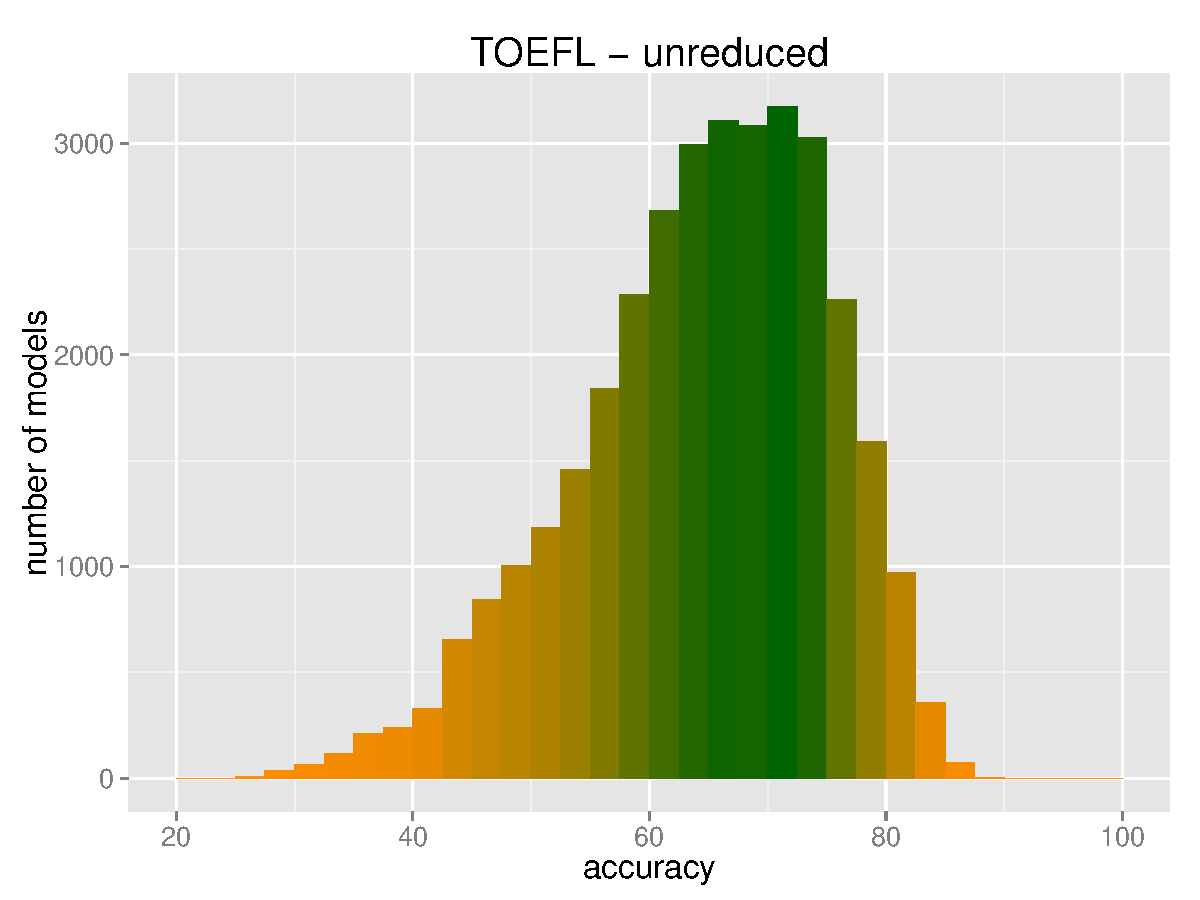
\includegraphics[scale=0.30]{img/lapesa_hist_toefl_unreduced}
      \begin{block}{}\footnotesize \centering
        Min:  25 ; Max: 87.5 ;  Mean: 63.9
      \end{block}
    \end{column}
    \begin{column}{0.5\textwidth}
      \hspace*{-18pt} 
      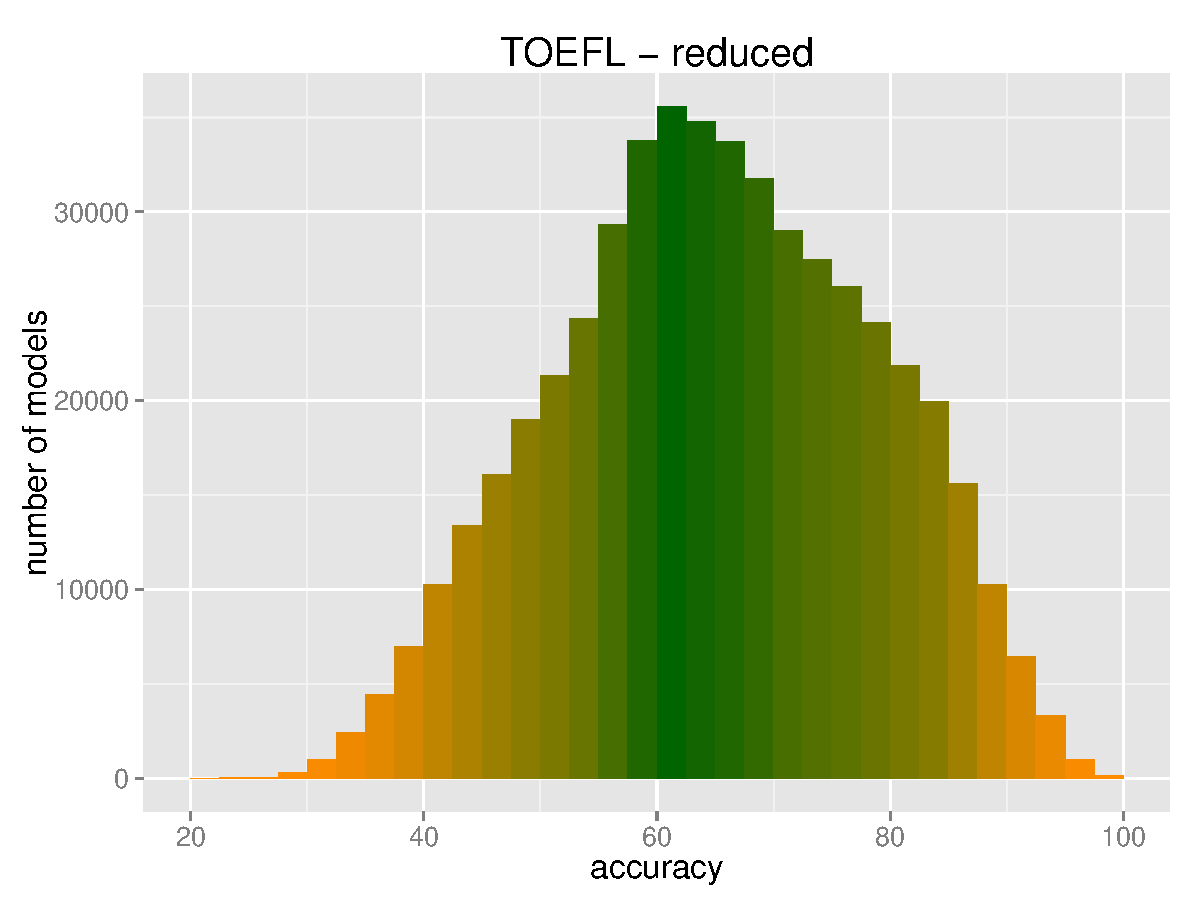
\includegraphics[scale=0.30]{img/lapesa_hist_toefl_reduced}
      \begin{block}{}\footnotesize \centering
        Min:  18.7; Max: \textbf{97.4};  Mean: 64.4
      \end{block}
    \end{column}
  \end{columns}
\end{frame}

\begin{frame}
  \frametitle{TOEFL task: Parameters and Explained Variance}
  \framesubtitle{Reduced setting: feature Ablation  (model $R^{2}$: 89\%)}
  \centering
  \hspace*{-10pt}
  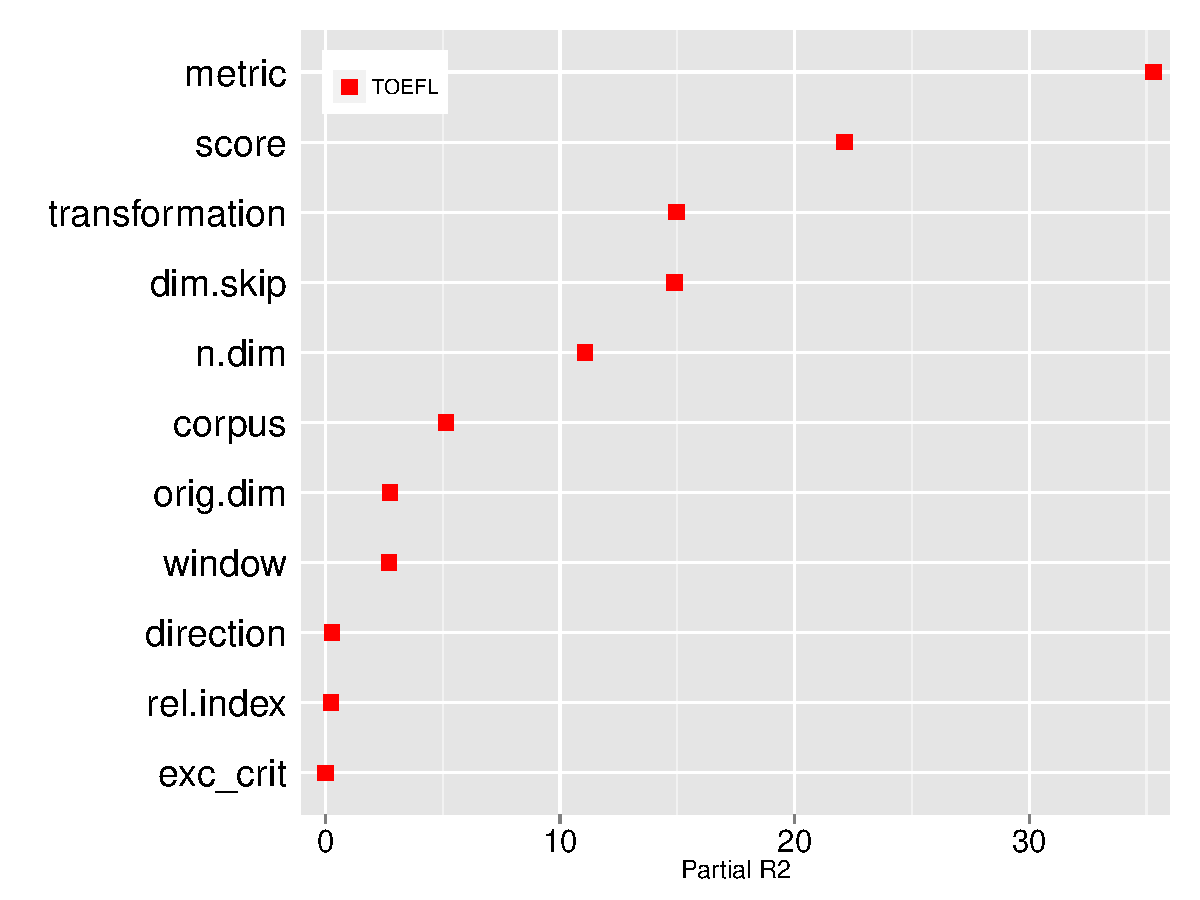
\includegraphics[scale=0.45]{img/lapesa_toefl_main_r2_reduced}

\end{frame}

\begin{frame}
  \frametitle{TOEFL task: Interactions}
  \framesubtitle{Reduced setting ($R^{2}$ $>$ 0.5)}

  \begin{center}
    \begin{tabular}{lrrrr}
      Interaction & Df &  R$^2$  \\ \hline
      \primary{score:transformation} & 18  & 7.42 \\   
      \primary{metric:dim.skip} & 2  & 4.44 \\ 
      \primary{score:metric} & 6  & 1.77 \\ 
      metric:orig.dim & 4  & 0.98 \\ 
      window:transformation & 12  & 0.91 \\     
      corpus:score & 12  & 0.84 \\  
      score:orig.dim & 24  & 0.64  \\ 
      metric:n.dim & 4  & 0.63  \\ 
    \end{tabular}

    \gap[1]
    \secondary{TOEFL task: interactions, $R^2$}
  \end{center}
  
\end{frame}



\begin{frame}
  \frametitle{TOEFL task: Partial Effects}
  \framesubtitle{Most Explanatory Parameters: Metric, Score, Transformation} 
  
  \begin{columns}
    
    \begin{column}{0.5\textwidth}
      \hspace*{-18pt} 
      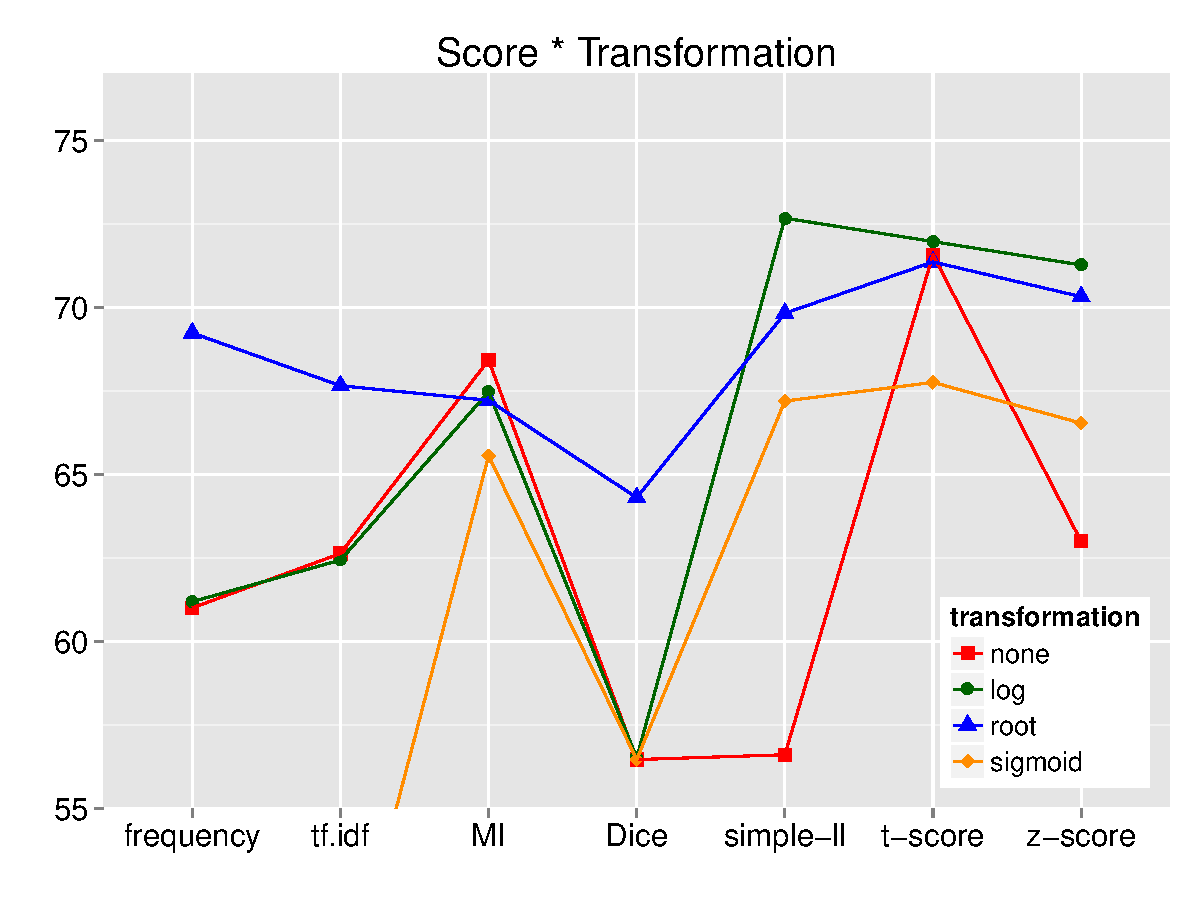
\includegraphics[scale=0.30]{img/lapesa_toefl_main_score_transformation}
    \end{column}


    \begin{column}{0.5\textwidth}
      \centering
      \hspace*{-18pt}   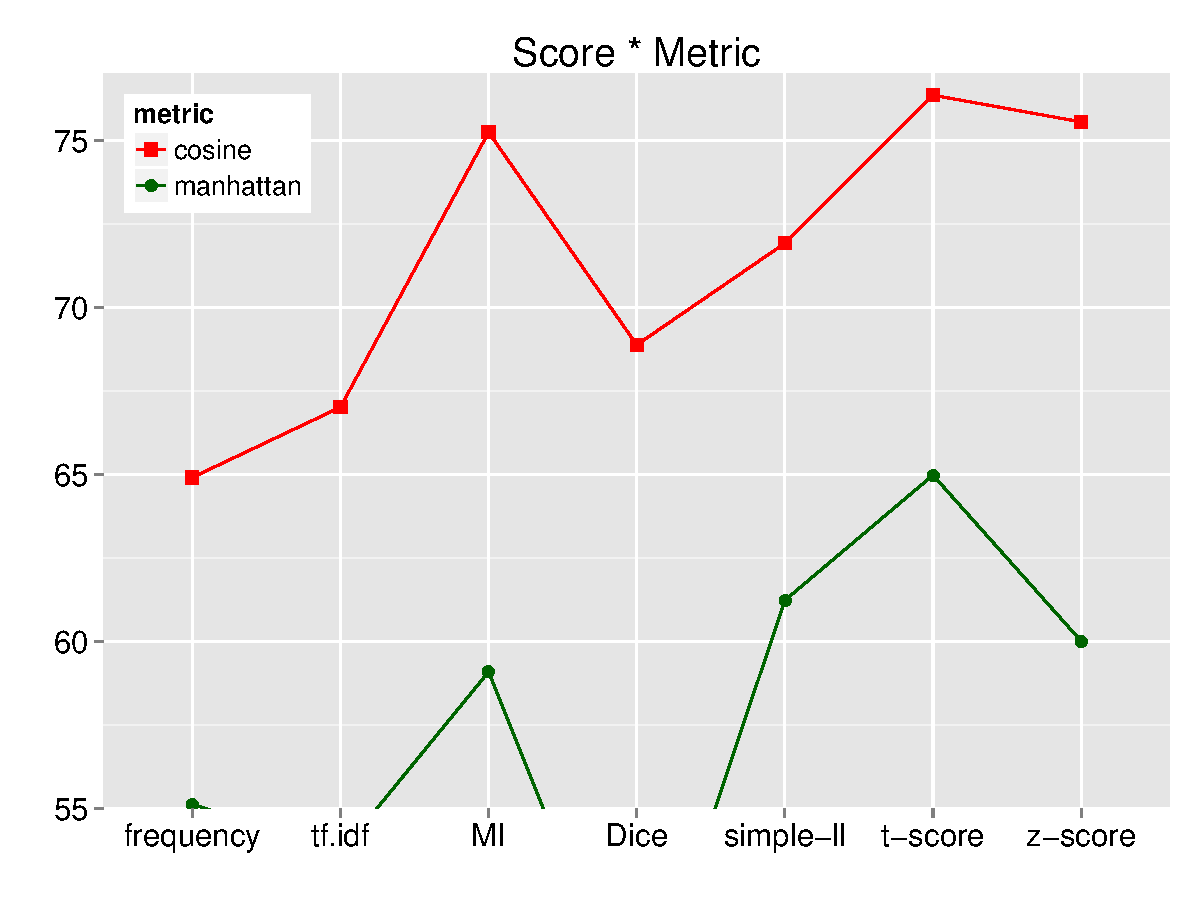
\includegraphics[scale=0.30]{img/lapesa_toefl_main_score_metric}

    \end{column}
  \end{columns}  
  
\end{frame}



\begin{frame}
  \frametitle{TOEFL task: Partial Effects}
  \framesubtitle{Most Explanatory Parameters: Dimensionality Reduction}
  \begin{columns}

    \begin{column}{0.5\textwidth}
      \centering
      \hspace*{-18pt}   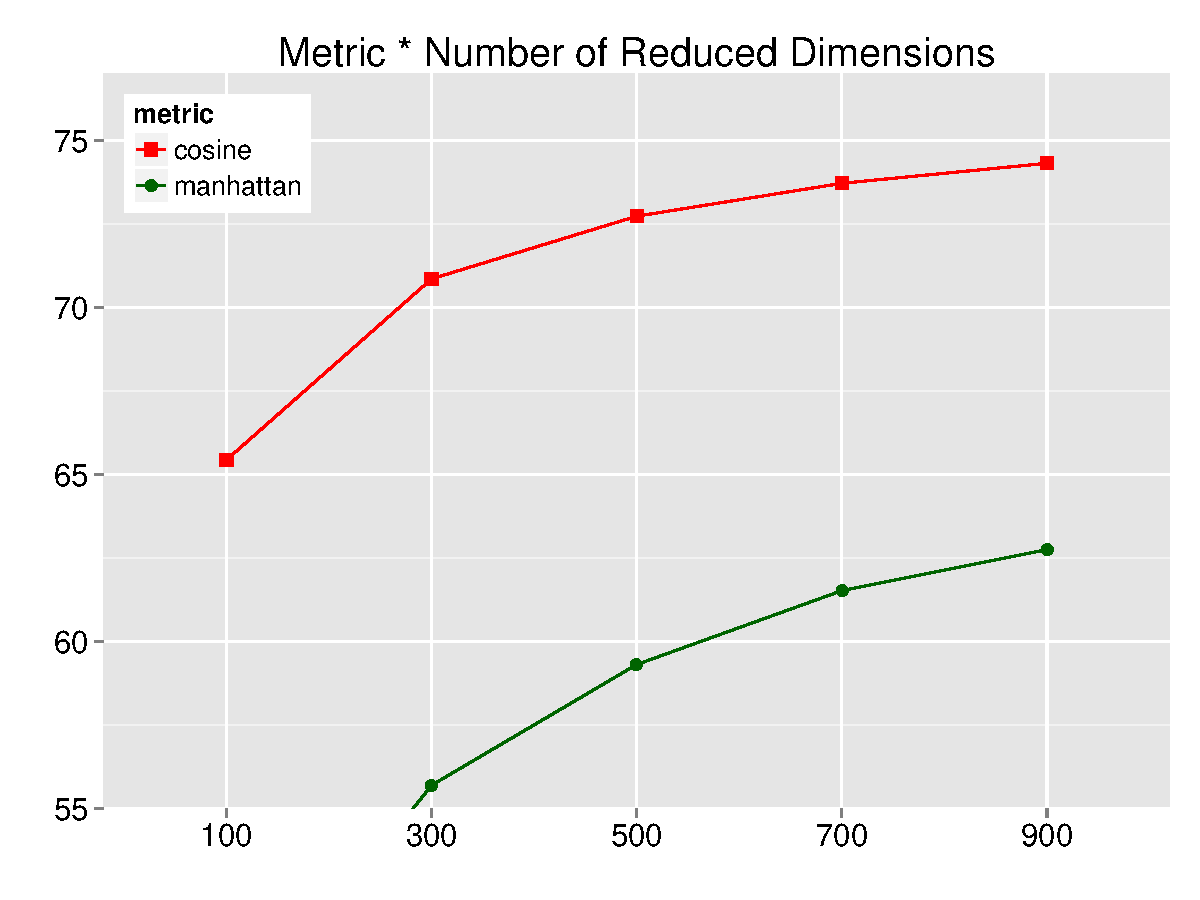
\includegraphics[scale=0.30]{img/lapesa_toefl_main_metric_n-dim}

    \end{column}
    \begin{column}{0.5\textwidth}
      \hspace*{-18pt} 
      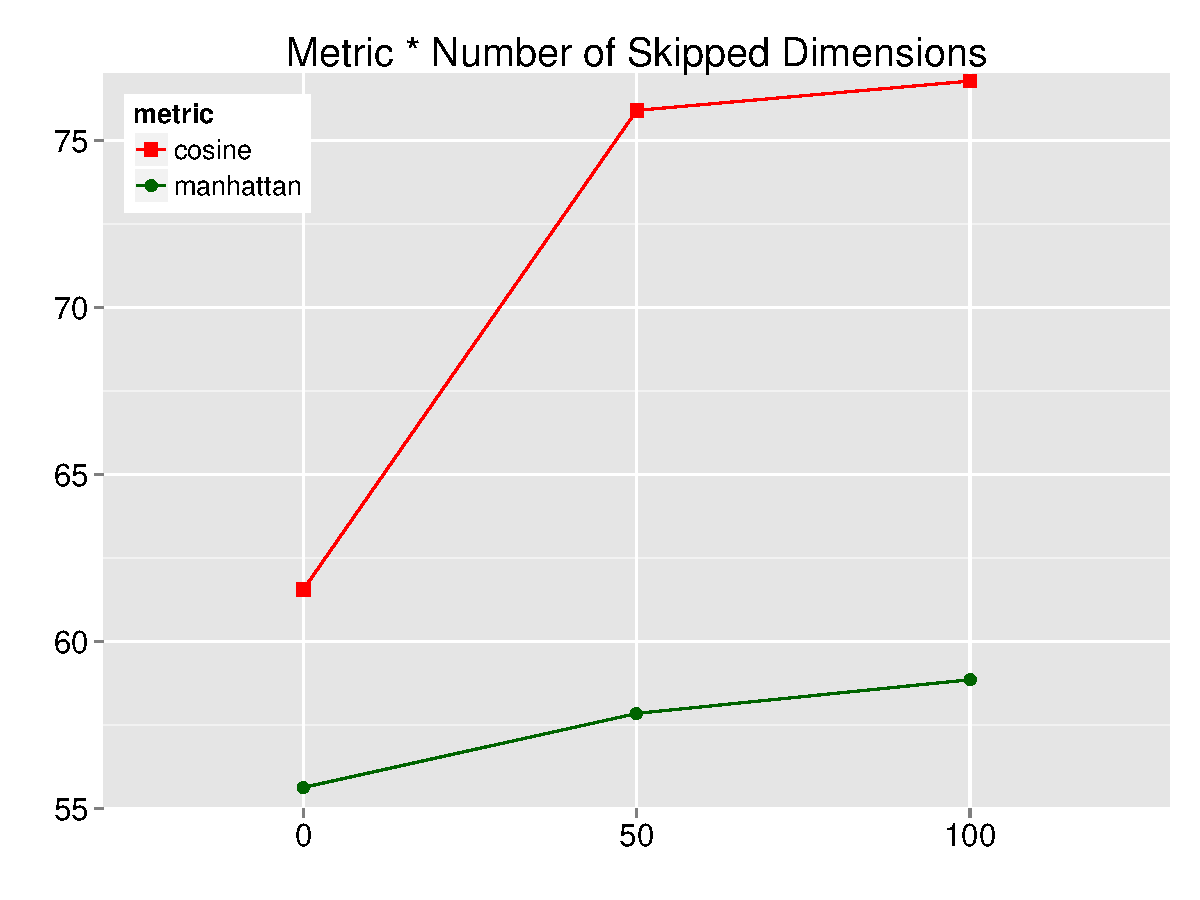
\includegraphics[scale=0.30]{img/lapesa_toefl_main_metric_dim-skip}
    \end{column}
  \end{columns}
  
\end{frame}


\begin{frame}
  \frametitle{TOEFL task: Partial Effects}
  \framesubtitle{Less Explanatory Parameters: Corpus and Number of Original Dimensions}
  \begin{columns}

    \begin{column}{0.5\textwidth}
      \centering
      \hspace*{-18pt}   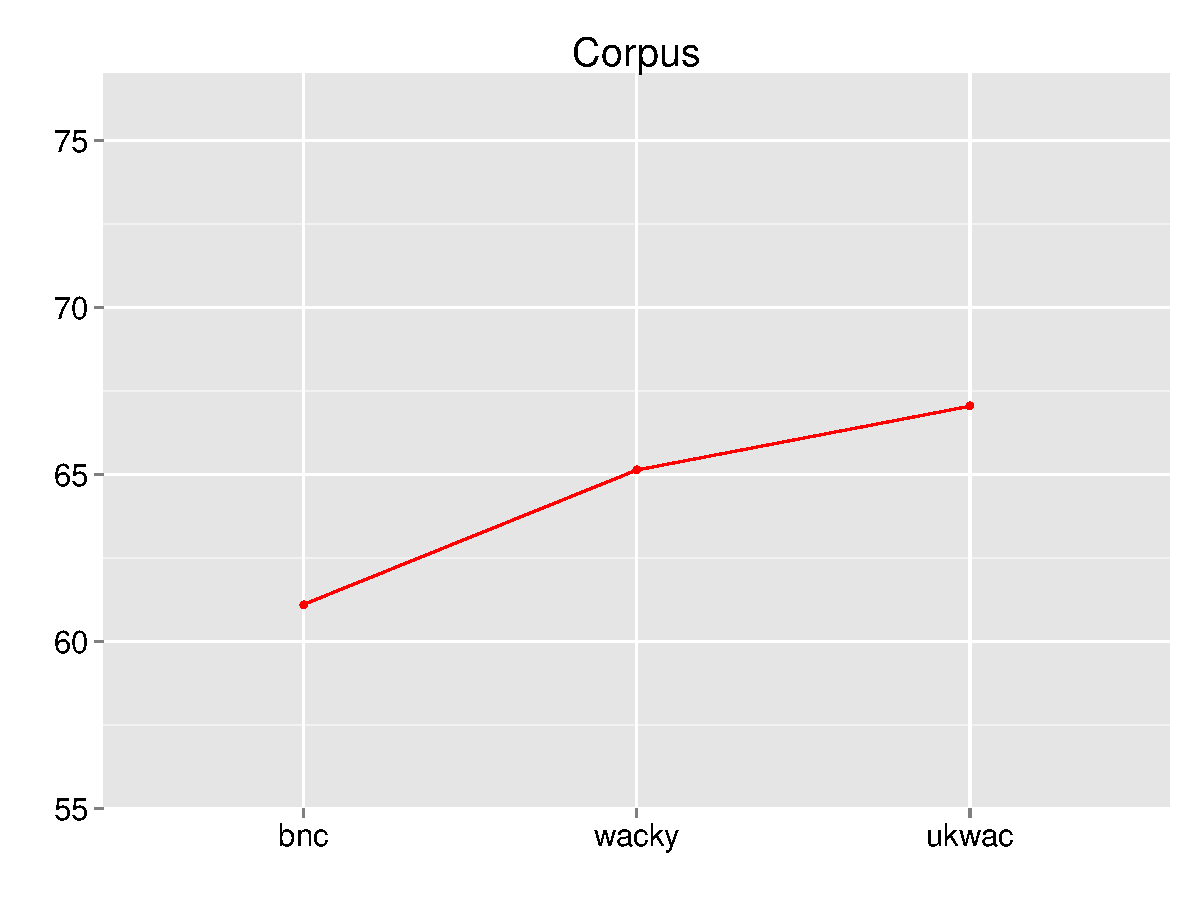
\includegraphics[scale=0.30]{img/lapesa_toefl_main_corpus}

    \end{column}
    \begin{column}{0.5\textwidth}
      \hspace*{-18pt} 
      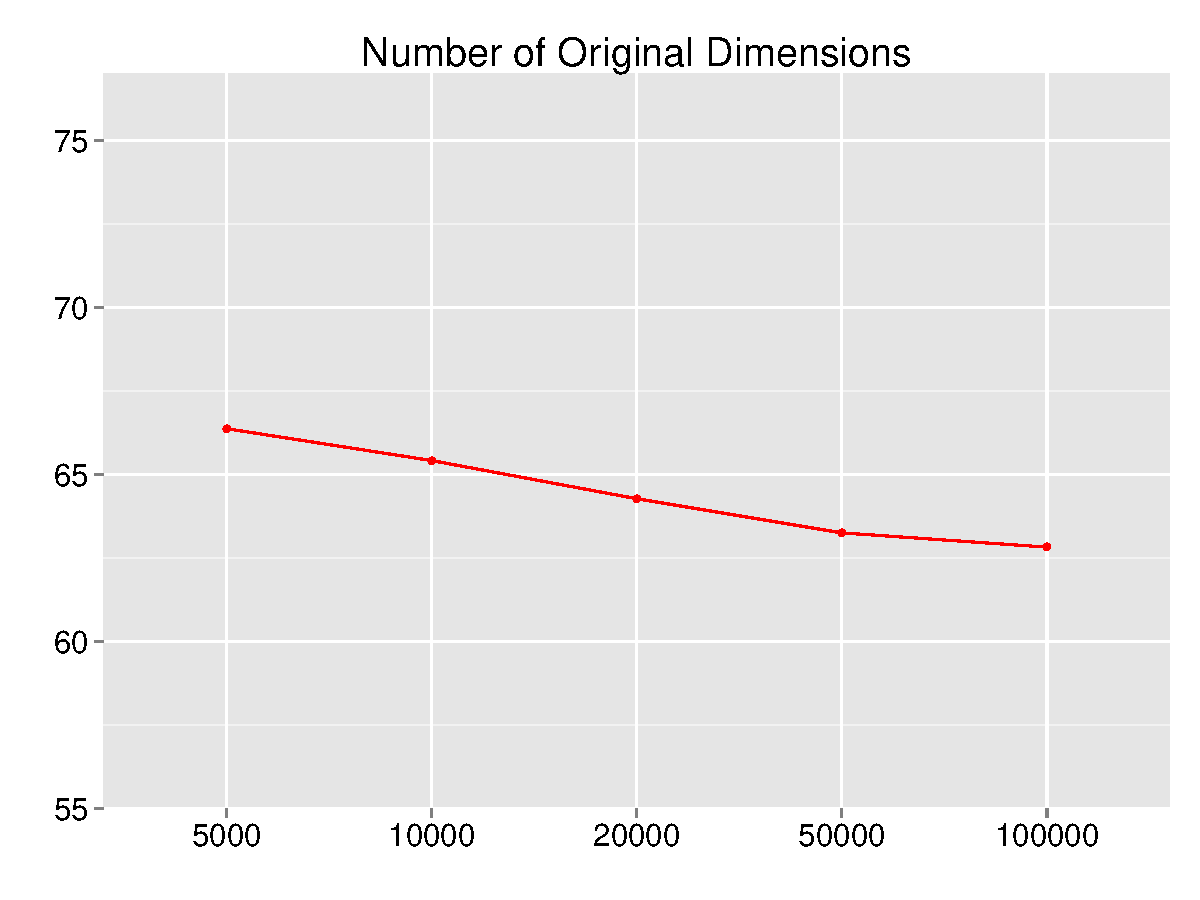
\includegraphics[scale=0.30]{img/lapesa_toefl_main_origdim}
    \end{column}
  \end{columns}
  
\end{frame}


\begin{frame}
  \frametitle{TOEFL task: Partial Effects}
  \framesubtitle{Less Explanatory Parameters: Window and Relatedness Index}
  \begin{columns}

    \begin{column}{0.5\textwidth}
      \centering
      \hspace*{-18pt}   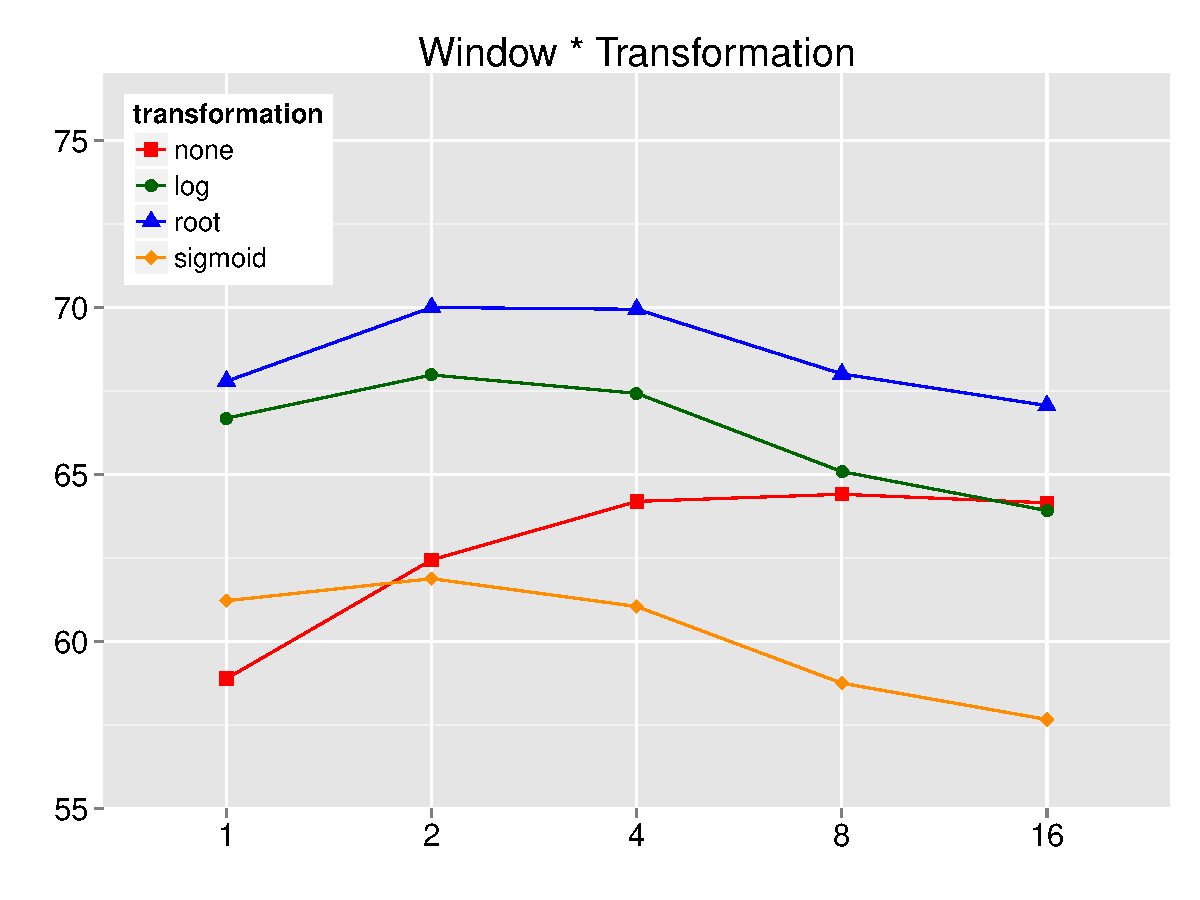
\includegraphics[scale=0.30]{img/lapesa_toefl_main_window_transformation}

    \end{column}
    \begin{column}{0.5\textwidth}
      \hspace*{-18pt} 
      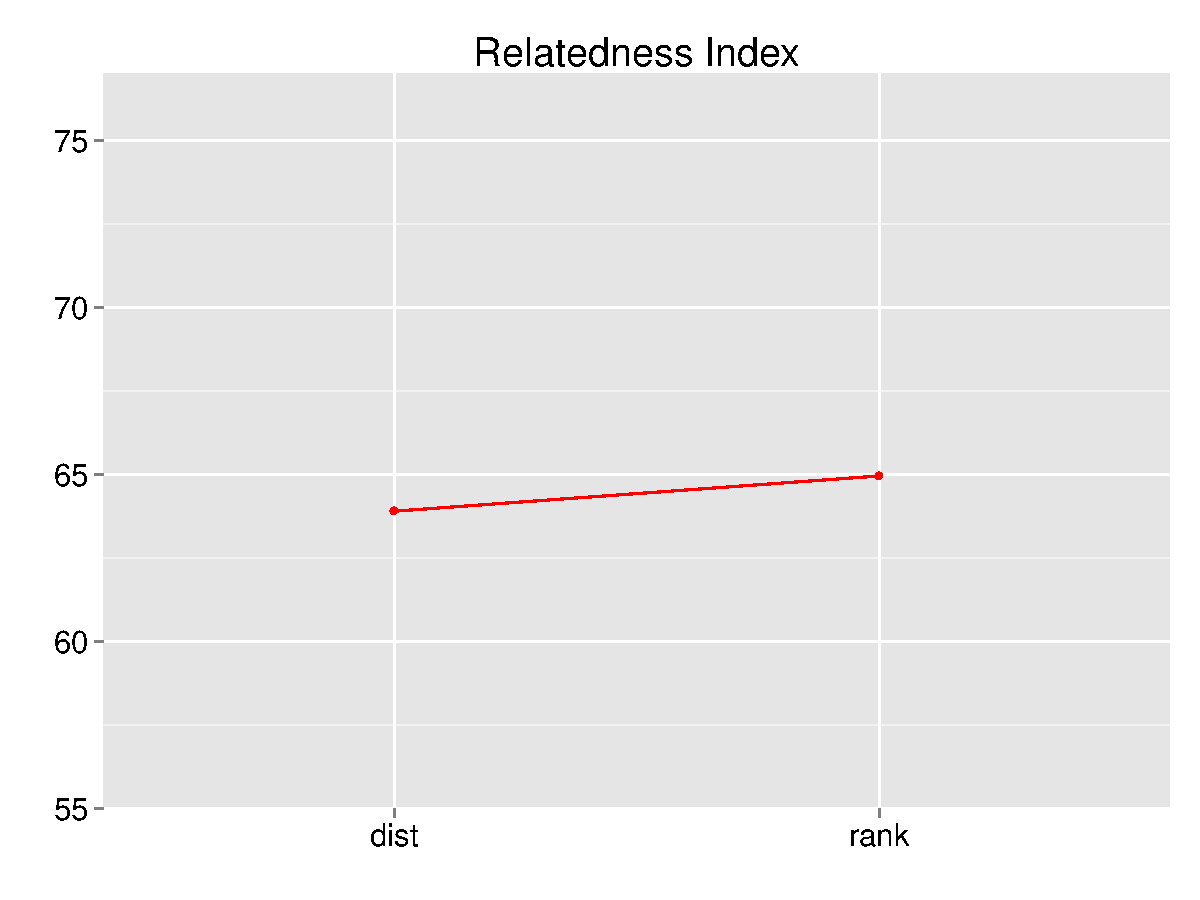
\includegraphics[scale=0.30]{img/lapesa_toefl_main_relindex}
    \end{column}
  \end{columns}
  
\end{frame}

\begin{frame}
  \frametitle{TOEFL task: summing up}
  \begin{exampleblock}{TOEFL: best setting}
    \begin{itemize}\footnotesize
    \item Corpus: ukWac
    \item Window: undirected, 2 words 
    \item Feature selection: top 5000/10000 dimensions, based on frequency
    \item Score * Transformation: simple-ll * log
    \item Dimensionality Reduction: 900 latent dimensions, skipping the first 100
    \item Distance Metric: cosine
    \item Index of Distributional Relatedness: neighbor rank
    \end{itemize}
  \end{exampleblock}   
  
\end{frame}


\begin{frame}
  \frametitle{DSMs and Similarity Ratings}
  \framesubtitle{Introducing the task}

  \ungap[1]
  \begin{columns}
    \begin{column}{0.5\textwidth}
      \begin{exampleblock}{RG65}
        \textbf{65 pairs, rated from 0 to 4}
        \textit{gem -- jewel}: 3.94 \\
        \textit{grin -- smile}:  3.46 \\
        \textit{fruit -- furnace}: 0.05 \\
      \end{exampleblock}
    \end{column}
    % 
    \begin{column}{0.5\textwidth}
      
      
      \begin{exampleblock}  {WordSim353}
        \textbf{353 pairs, rated from 1 to 10}
        \textit{announcement -- news}: 7.56 \\
        \textit{weapon -- secret}:  6.06 \\
        \textit{travel -- activity}: 5.00 \\
      \end{exampleblock}
    \end{column}
    % 
  \end{columns}
  % 
  % 
  \begin{itemize}
  \item A \textbf{prediction} task
  \item If distributional representation are close to  speakers' conceptual representations, we expect to find some \textbf{correlation} between distance in the semantic space and speaker's judgments concerning semantic similarity
  \item Performance: \textbf{Pearson correlation $r$}
  \end{itemize}

\end{frame}

\begin{frame}
  \frametitle{Correlation to Similarity Ratings: Performance}
  \framesubtitle{Rubenstein and Goodenough dataset: Unreduced versus reduced experiments}
  \centering
  
  \begin{columns}
    \begin{column}{0.5\textwidth}
      \centering
      \hspace*{-18pt}   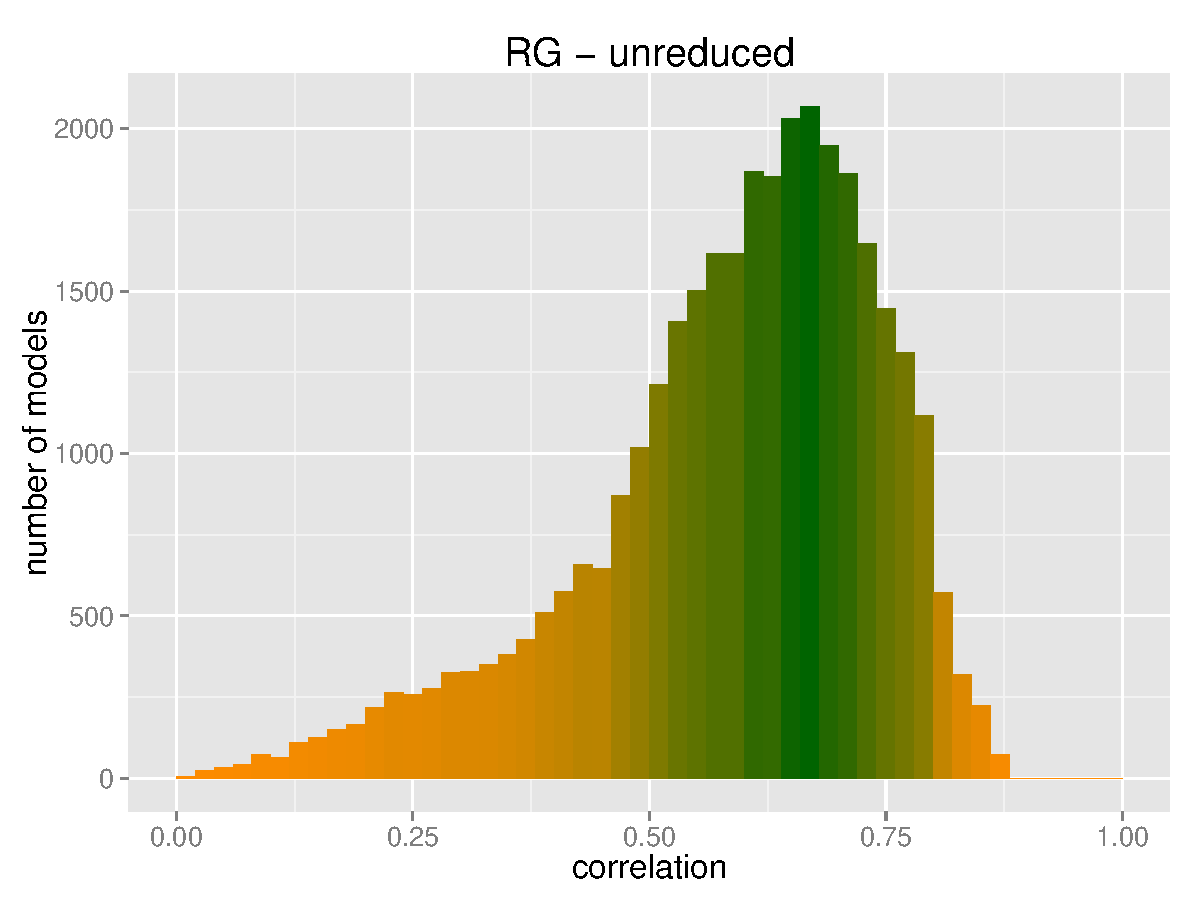
\includegraphics[scale=0.30]{img/lapesa_hist_rg_unreduced}
      \begin{block}{}\footnotesize \centering
        Min:  0.01 ; Max:  0.88;  Mean 0.59 
      \end{block}
    \end{column}
    \begin{column}{0.5\textwidth}
      \hspace*{-18pt} 
      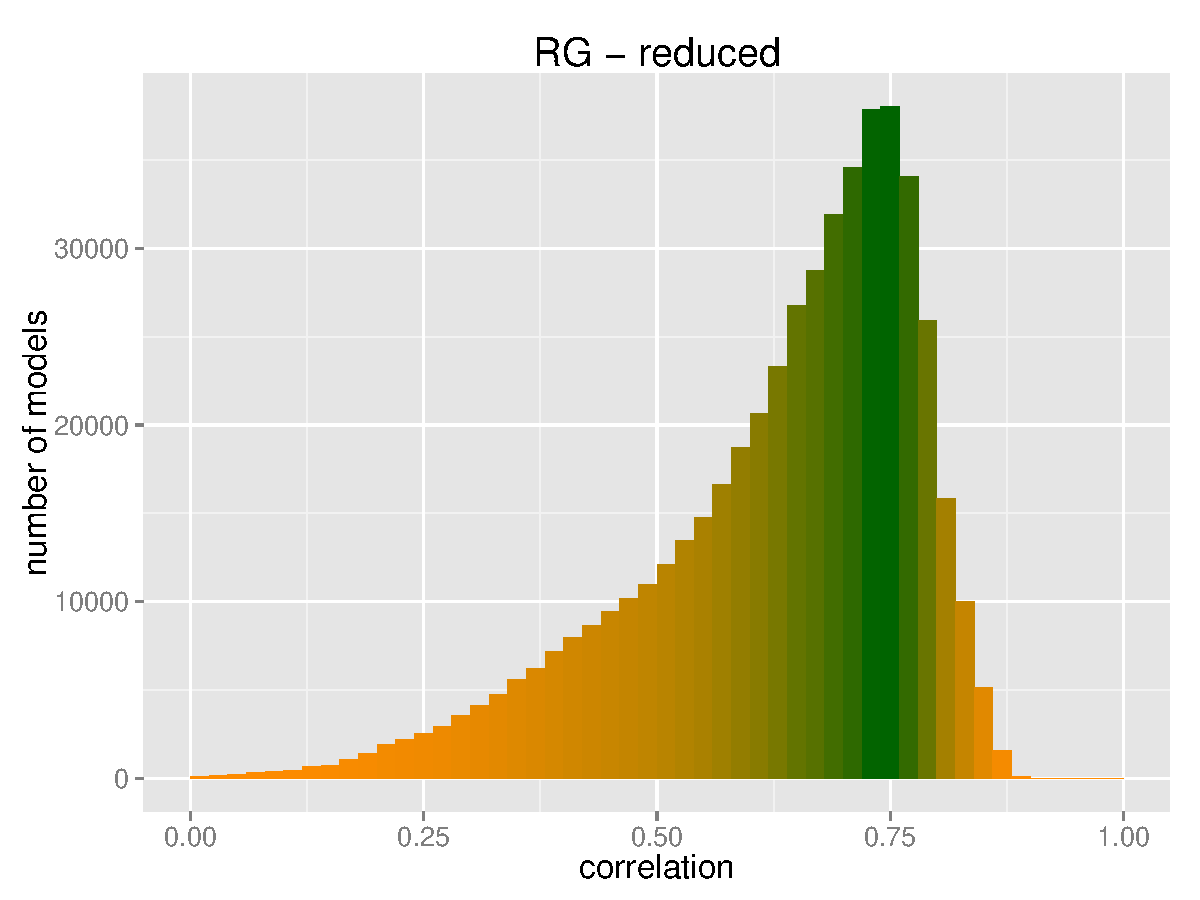
\includegraphics[scale=0.30]{img/lapesa_hist_rg_reduced}
      \begin{block}{}\footnotesize \centering
        Min:  0.00; Max: \textbf{0.89};  Mean: 0.63
      \end{block}
    \end{column}
  \end{columns}
 
\end{frame}


\begin{frame}
  \frametitle{Correlation to Similarity Ratings: Performance}
  \framesubtitle{WordSim353 dataset: Unreduced versus reduced experiments}
  \centering
  
  \begin{columns}

    \begin{column}{0.5\textwidth}
      \centering
      \hspace*{-18pt} 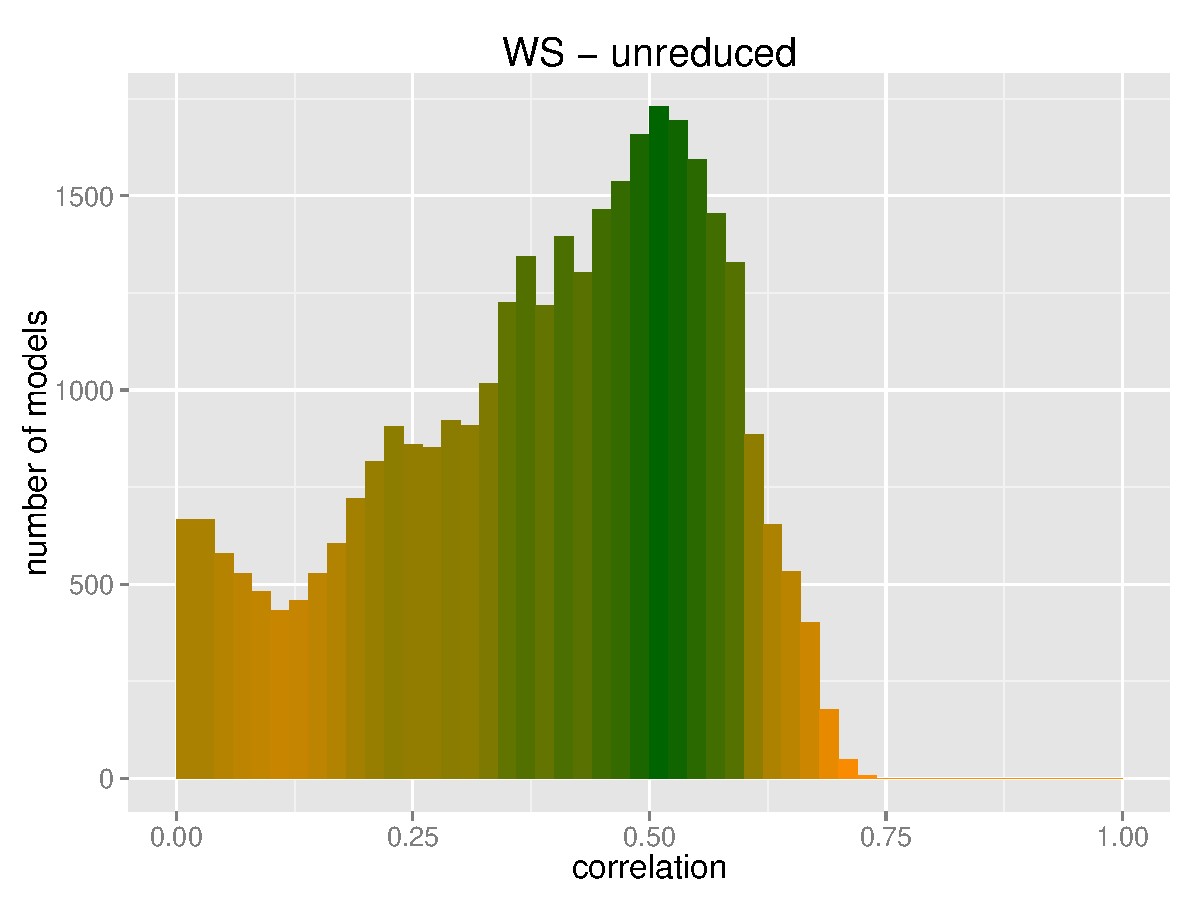
\includegraphics[scale=0.30]{img/lapesa_hist_ws_unreduced}
      \begin{block}{}\footnotesize \centering
        Min:  0.00; \textbf{Max:  0.73};  Mean: 0.39
      \end{block}
    \end{column}
    \begin{column}{0.5\textwidth}
      \hspace*{-18pt} 
      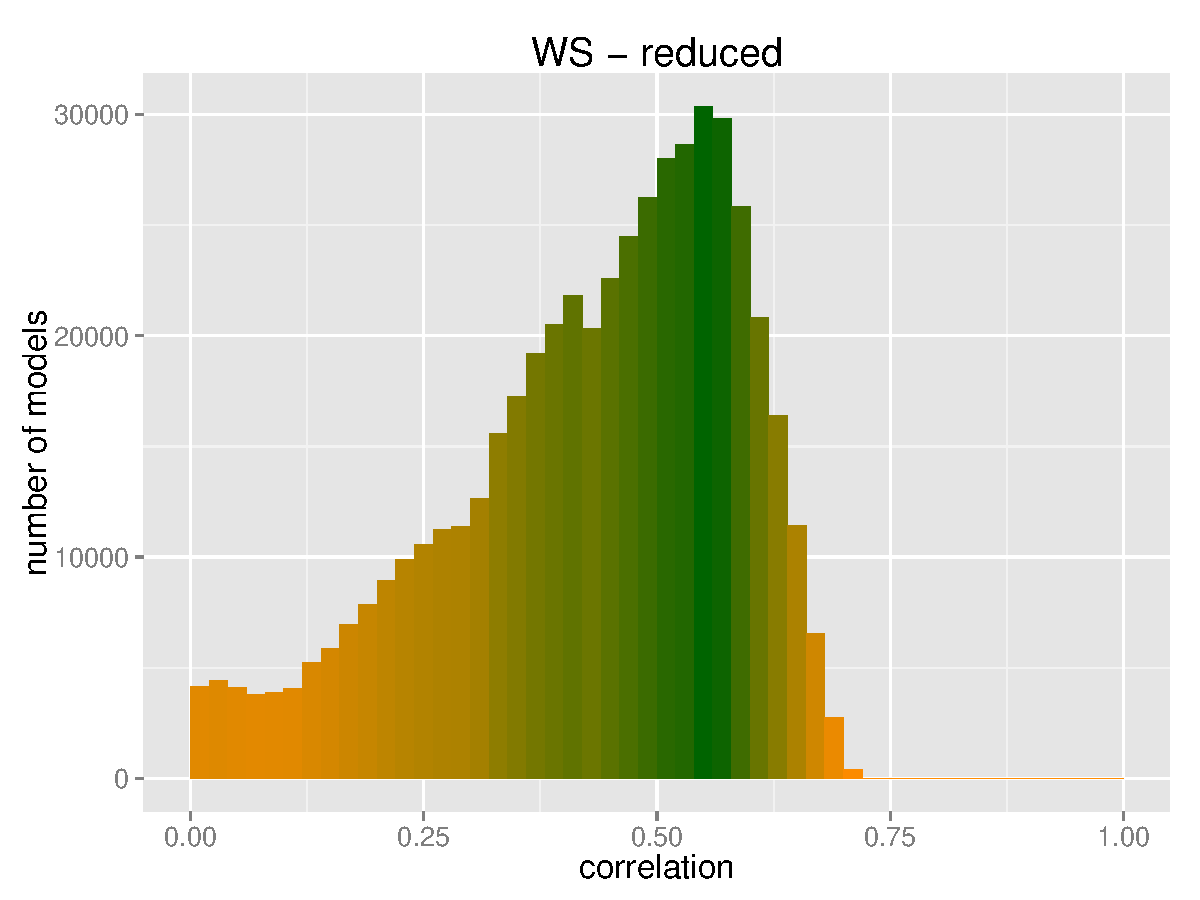
\includegraphics[scale=0.30]{img/lapesa_hist_ws_reduced}
      \begin{block}{}\footnotesize \centering
        Min:  0.00; Max: \textbf{0.73};  Mean: 0.43
      \end{block}
    \end{column}
  \end{columns}  
\end{frame}


\begin{frame}
  \frametitle{Correlation to Ratings: Parameters and Explained Variance}
  \framesubtitle{Reduced setting: feature Ablation  (model $R^{2}$:  RG65 86\%; WS353 90\%)}
  \centering
  \hspace*{-10pt}
  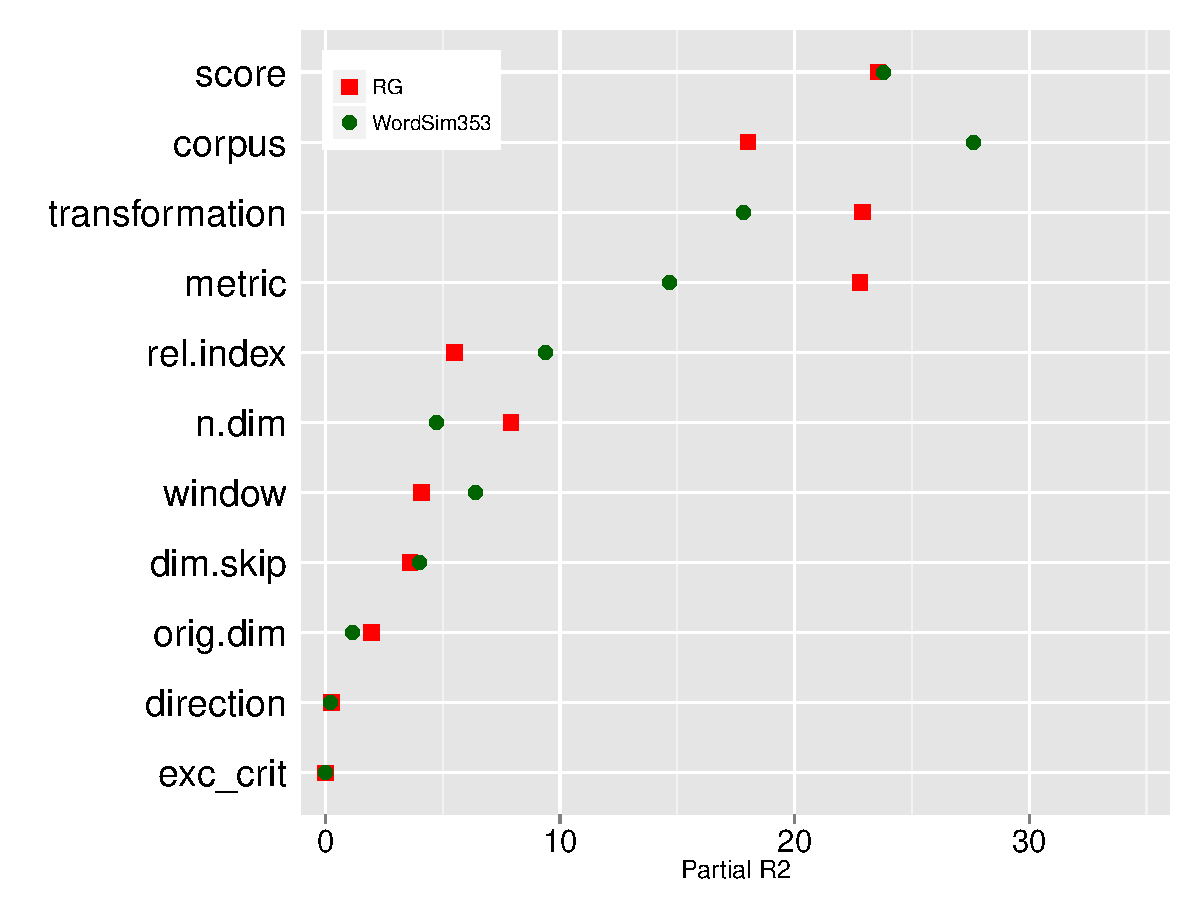
\includegraphics[scale=0.45]{img/lapesa_ratings_main_r2_reduced}

\end{frame}

\begin{frame}
  \frametitle{Correlation to Ratings: Interactions}
  \framesubtitle{Reduced setting ($R^{2}$ $>$ 0.5 )}

  \begin{center}
    \begin{tabular}{lrrrr}
      Interaction & Df & RG65  & WordSim353 \\ \hline

      \primary{score:transf} & 18  & 10.28 & 8.66  \\ 
      \primary{metric:n.dim} & 4  & 2.18 & 1.42 \\   
      \primary{window:transf} & 12  & 1.43 & 1.01 \\   
      corpus:metric & 2  & 1.83 & 0.51 \\  
      score:metric & 6  & 1.91 & 0.59  \\  
      metric:orig.dim & 4  & 1.08 & 0.62 \\ 
      corpus:score & 12 & 0.77 &  0.82 \\ 
      window:score & 24  & 0.77 & 0.69  \\
      score:dim.skip & 12  & 0.58 & 0.85 \\ 
    \end{tabular}

    \gap[1]
    \secondary{Rating datasets: interactions, $R^2$} 
  \end{center}

\end{frame}



\begin{frame}
  \frametitle{Correlation to Ratings: Partial Effects}
  \framesubtitle{Most Explanatory Parameters:  Score, Transformation} 
  
  \begin{columns}
    
    \begin{column}{0.5\textwidth}
      \centering
      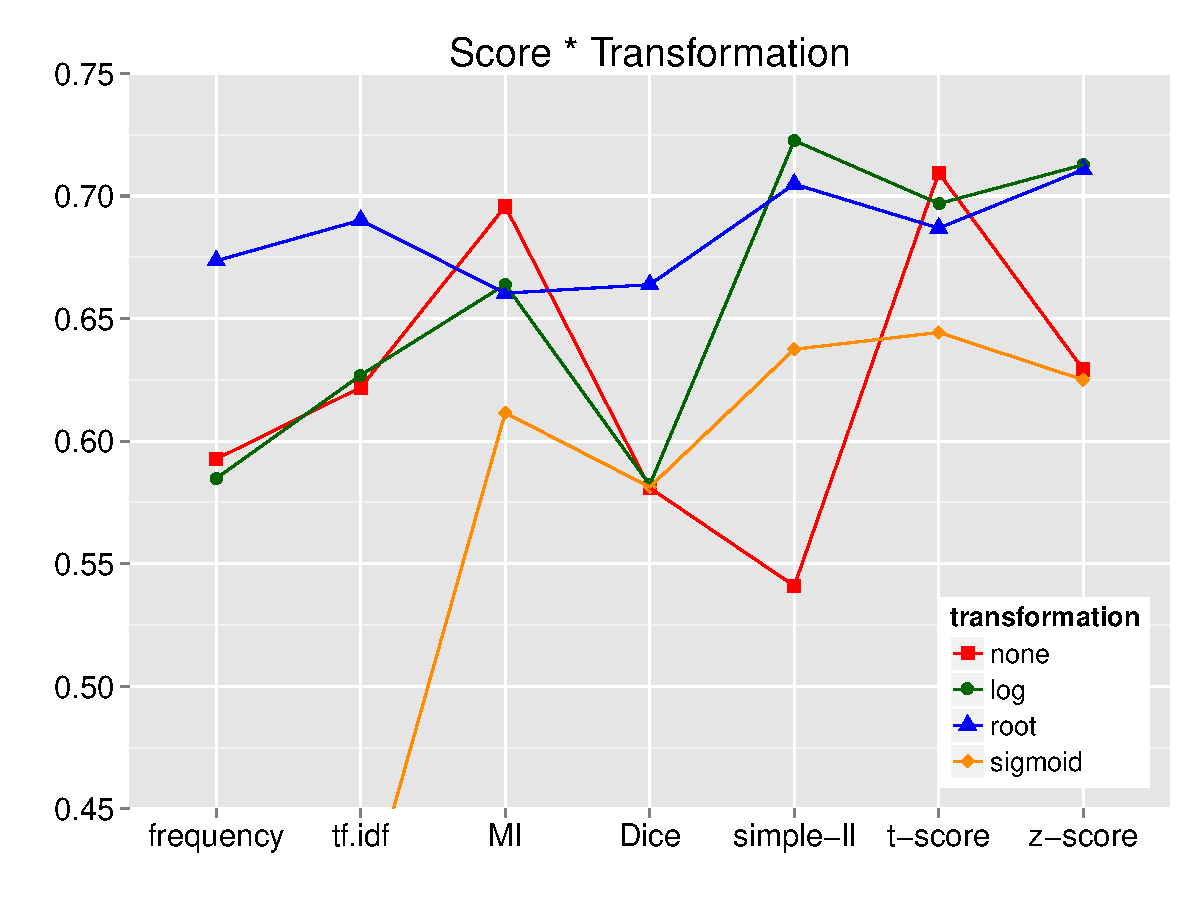
\includegraphics[scale=0.30]{img/lapesa_rg_main_score_transformation}

      \gap[1]
      \secondary{Rubenstein \& Goodenough}
    \end{column}


    \begin{column}{0.5\textwidth}
      \centering
      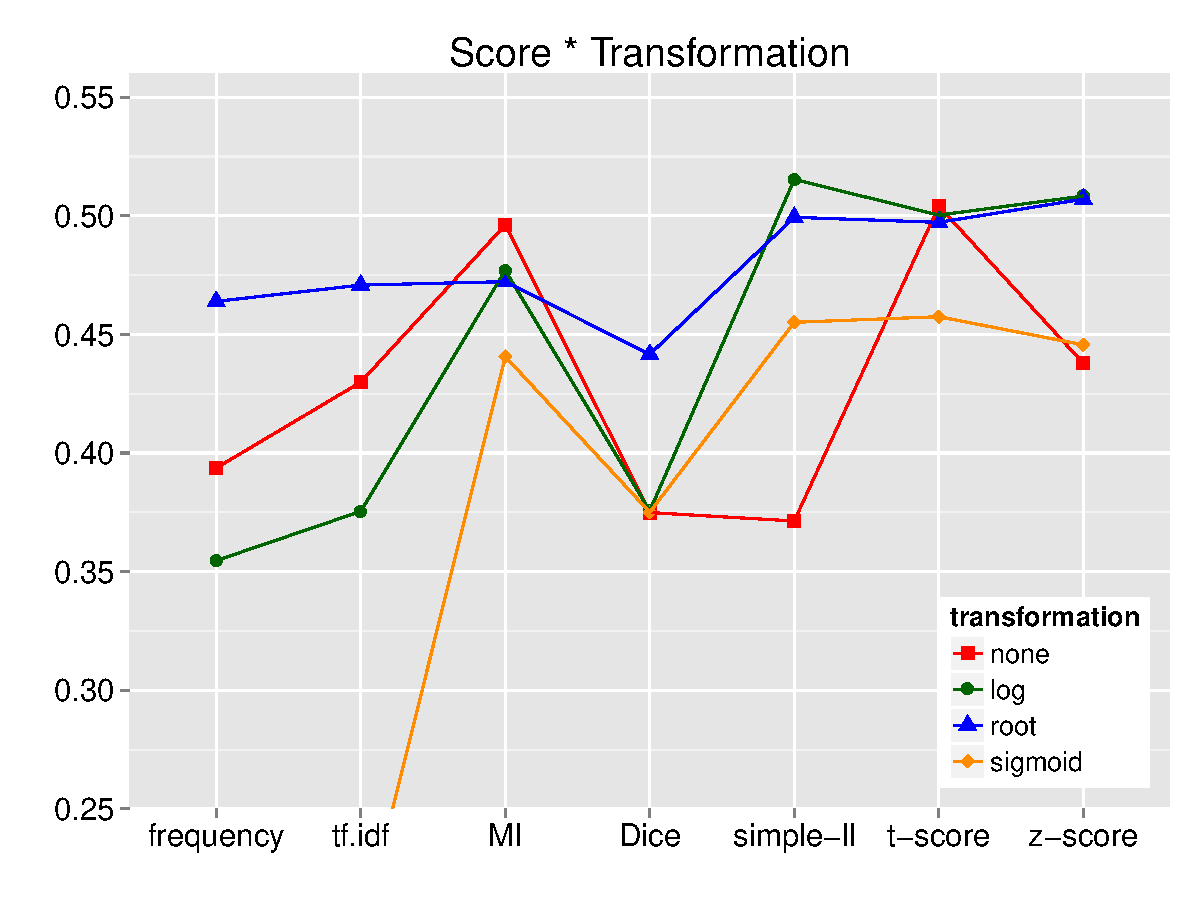
\includegraphics[scale=0.30]{img/lapesa_ws_main_score_transformation}
      
      \gap[1]
      \secondary{WordSim353}

    \end{column}
  \end{columns}  
  
\end{frame}

\begin{frame}
  \frametitle{Correlation to Ratings: Partial Effects}
  \framesubtitle{Most Explanatory Parameters:  Corpus} 
  
  \vspace{-18pt}
  
  \begin{columns}
    
    \begin{column}{0.5\textwidth}
      \begin{figure} 
        \hspace*{-18pt} 
        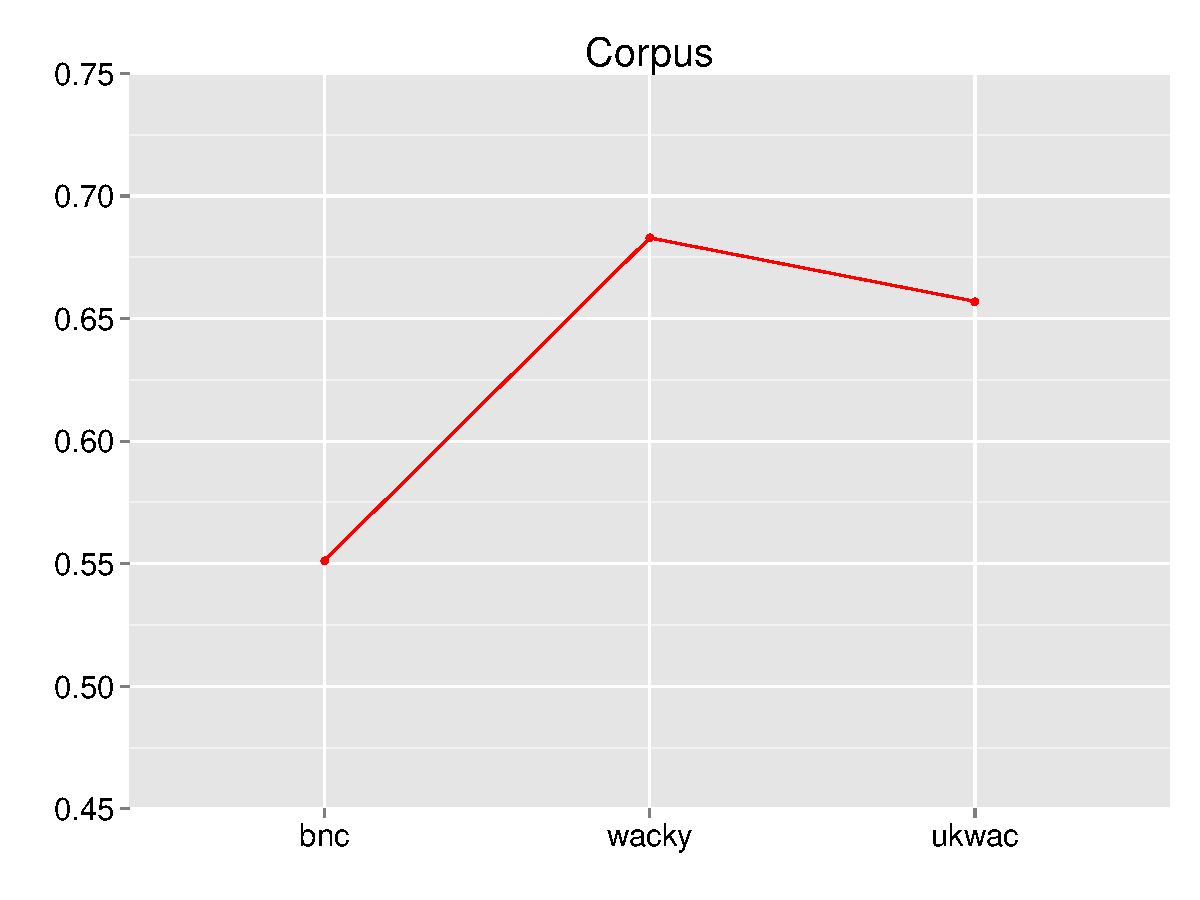
\includegraphics[scale=0.30]{img/lapesa_rg_main_corpus}
        \vspace{-10pt}
        \caption{Rubenstein Goodenough dataset}
      \end{figure}
    \end{column}


    \begin{column}{0.5\textwidth}
      \centering
      
      \begin{figure}
        \hspace*{-18pt}   
        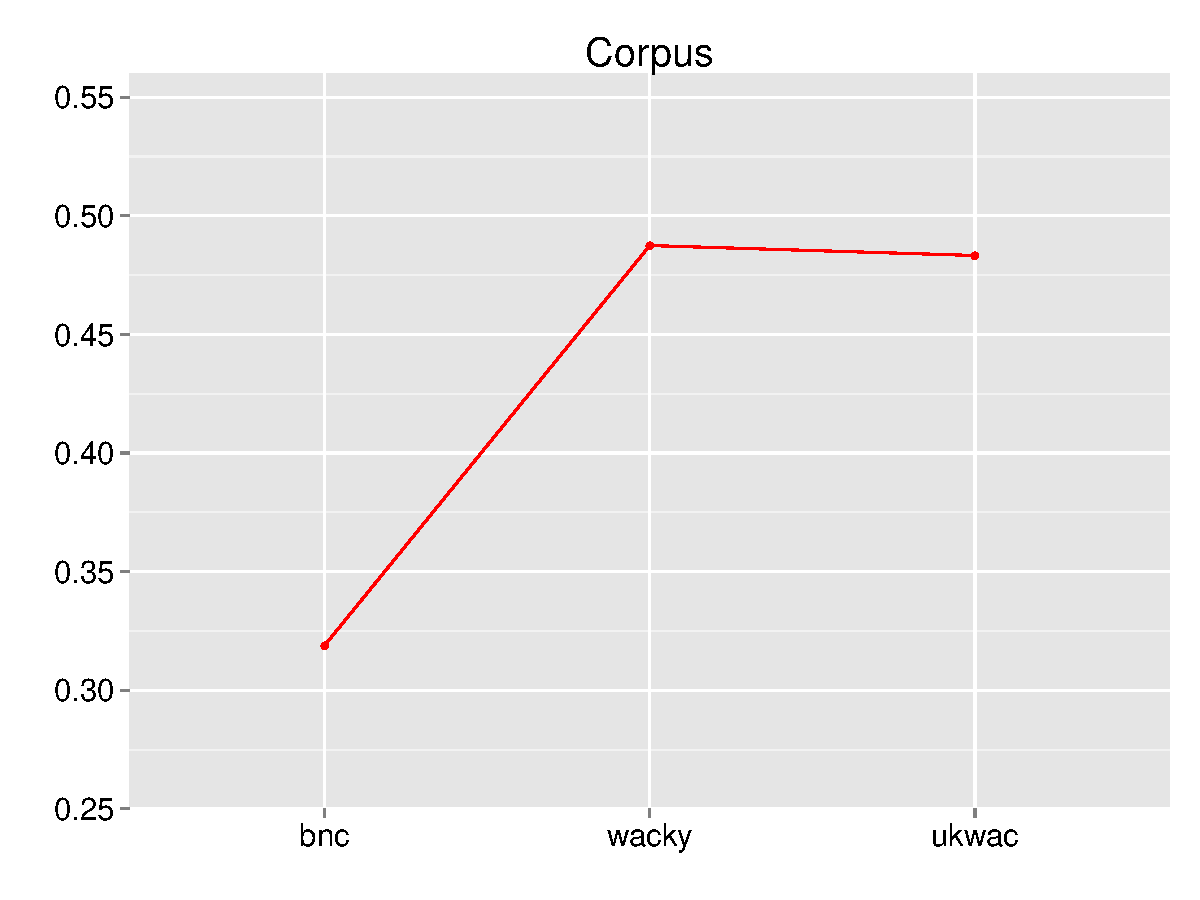
\includegraphics[scale=0.30]{img/lapesa_ws_main_corpus}
        \vspace{-10pt}
        \caption{WordSim353 dataset}
      \end{figure}
      
    \end{column}
  \end{columns}  
  
\end{frame}


\begin{frame}
  \frametitle{Correlation to Ratings: Partial Effects}
  \framesubtitle{Most Explanatory Parameters:  Relatedness Index} 
  
  \vspace{-18pt}
  
  \begin{columns}
    
    \begin{column}{0.5\textwidth}
      \begin{figure} 
        \hspace*{-18pt} 
        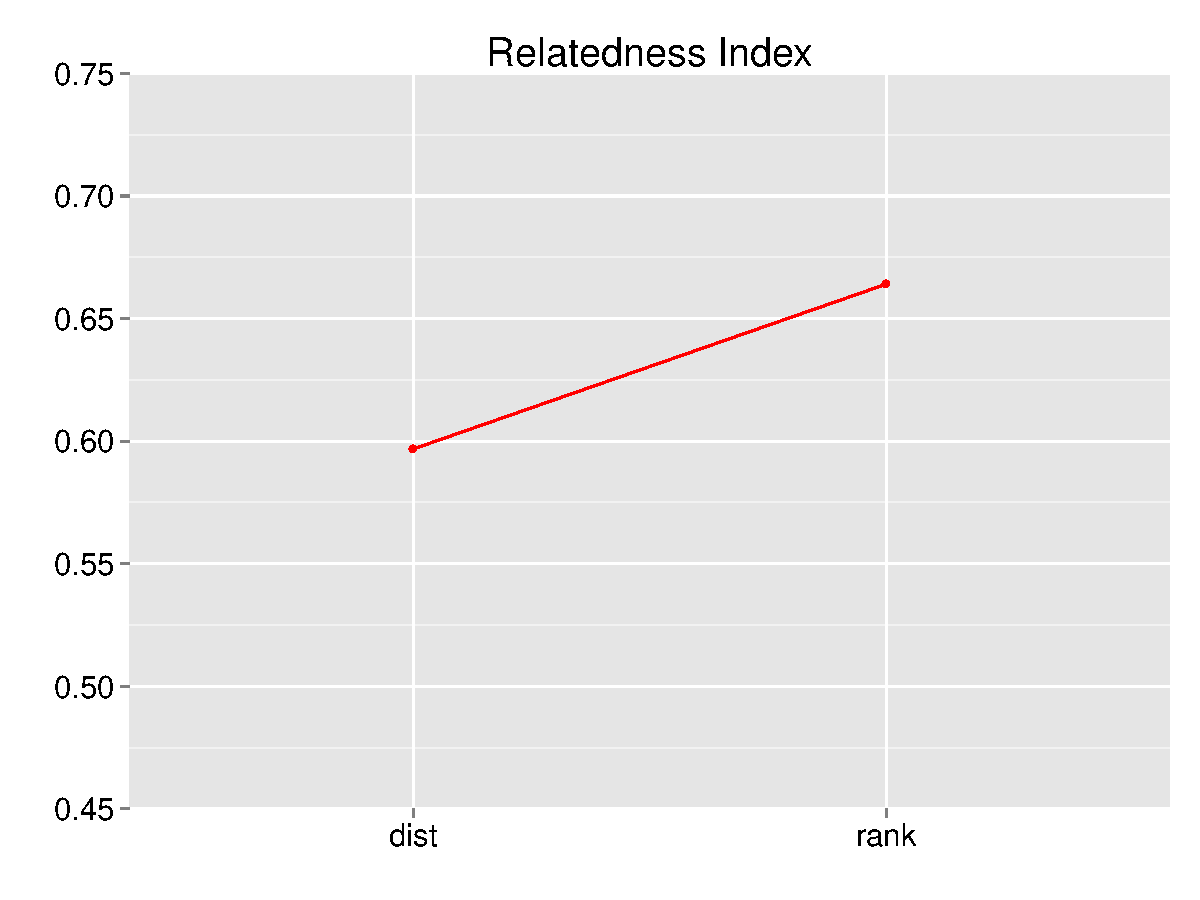
\includegraphics[scale=0.30]{img/lapesa_rg_main_relindex}
        \vspace{-10pt}
        \caption{Rubenstein Goodenough dataset}
      \end{figure}
    \end{column}


    \begin{column}{0.5\textwidth}
      \centering
      
      \begin{figure}
        \hspace*{-18pt}   
        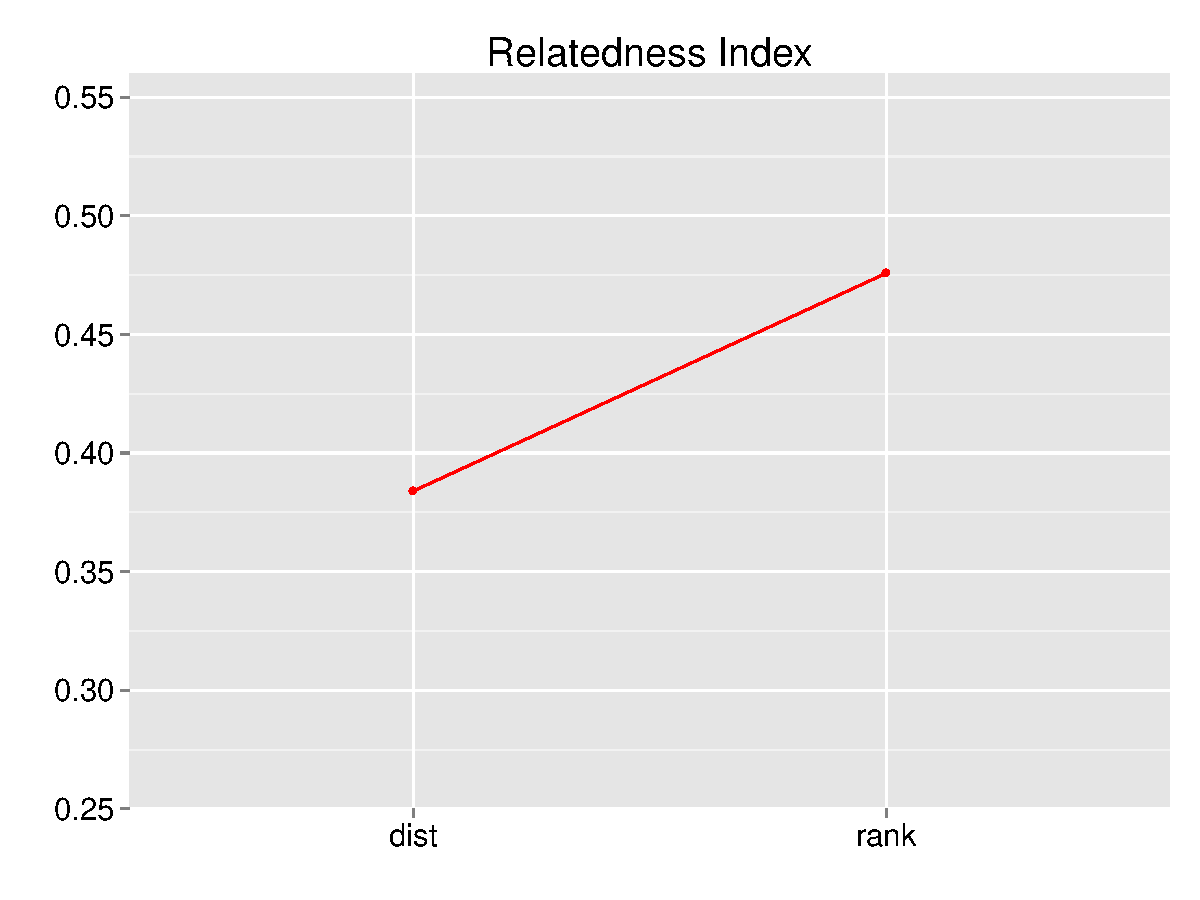
\includegraphics[scale=0.30]{img/lapesa_ws_main_relindex}
        \vspace{-10pt}
        \caption{WordSim353 dataset}
      \end{figure}
      
    \end{column}
  \end{columns}  
  
\end{frame}

\begin{frame}
  \frametitle{Correlation to Ratings: Partial Effects}
  \framesubtitle{Most Explanatory Parameters: Metric (* Number of Original Dimensions)}

  \vspace{-18pt}

  \begin{columns}
    
    \begin{column}{0.5\textwidth}
      \begin{figure} 
        \hspace*{-18pt} 
        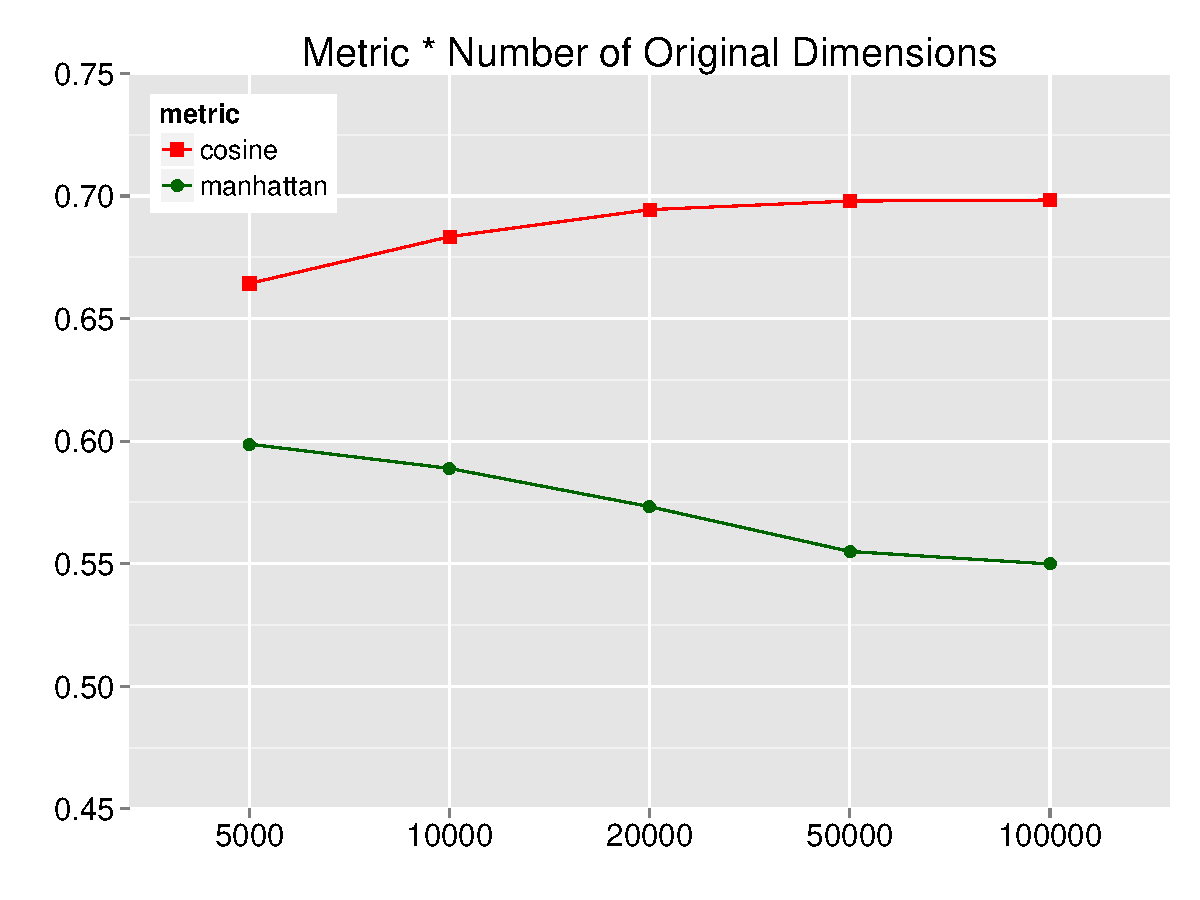
\includegraphics[scale=0.30]{img/lapesa_rg_main_metric_origdim}
        \vspace{-10pt}
        \caption{Rubenstein Goodenough dataset}
      \end{figure}
    \end{column}

    \begin{column}{0.5\textwidth}
      \centering
      
      \begin{figure}
        \hspace*{-18pt}   
        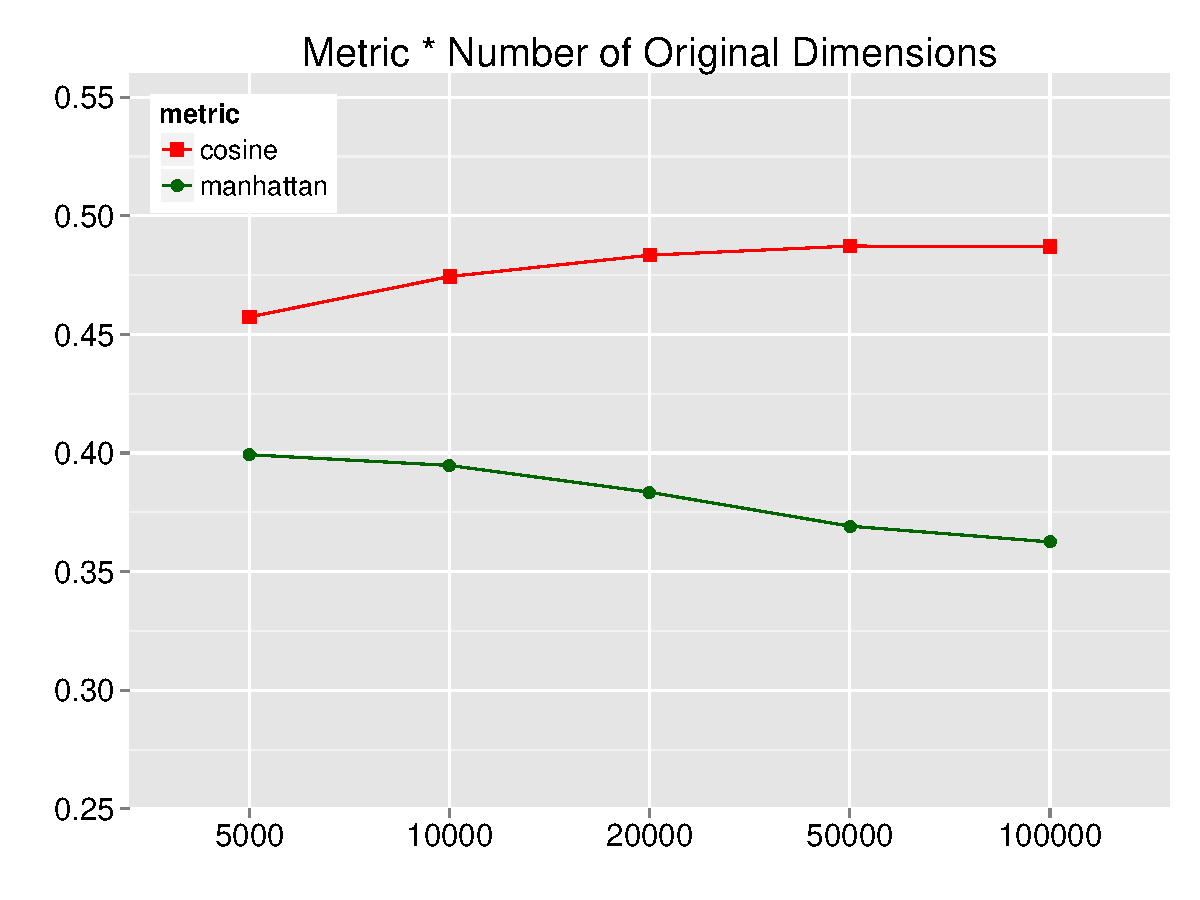
\includegraphics[scale=0.30]{img/lapesa_ws_main_metric_origdim}
        \vspace{-10pt}
        \caption{WordSim353 dataset}
      \end{figure}
      
    \end{column}
  \end{columns}  
  
\end{frame}



\begin{frame}
  \frametitle{Correlation to Ratings: Partial Effects}
  \framesubtitle{Quite Explanatory Parameters:  Number of Latent Dimensions} 
  
  \vspace{-18pt}
  
  \begin{columns}
    
    \begin{column}{0.5\textwidth}
      \begin{figure} 
        \hspace*{-18pt} 
        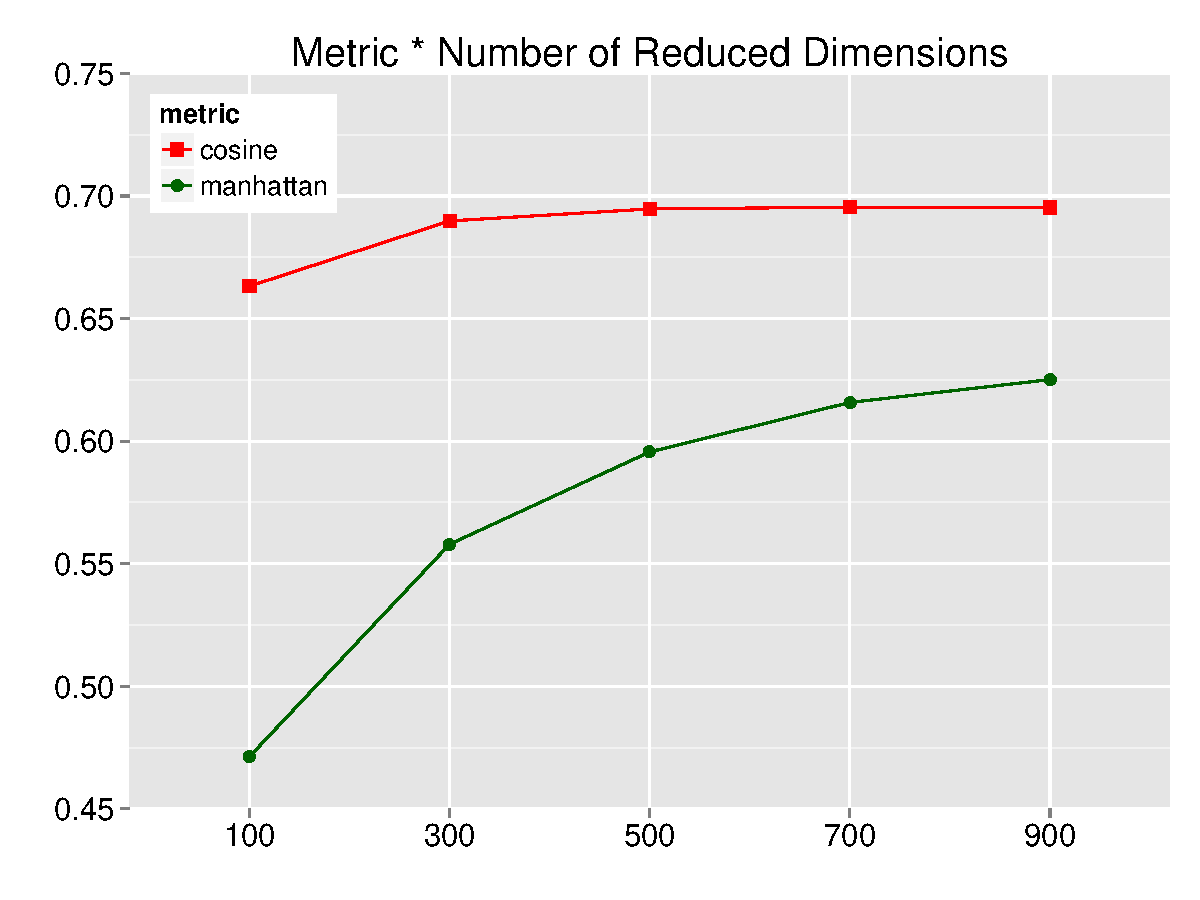
\includegraphics[scale=0.30]{img/lapesa_rg_main_metric_n-dim}
        \vspace{-10pt}
        \caption{Rubenstein Goodenough dataset}
      \end{figure}
    \end{column}


    \begin{column}{0.5\textwidth}
      \centering
      
      \begin{figure}
        \hspace*{-18pt}   
        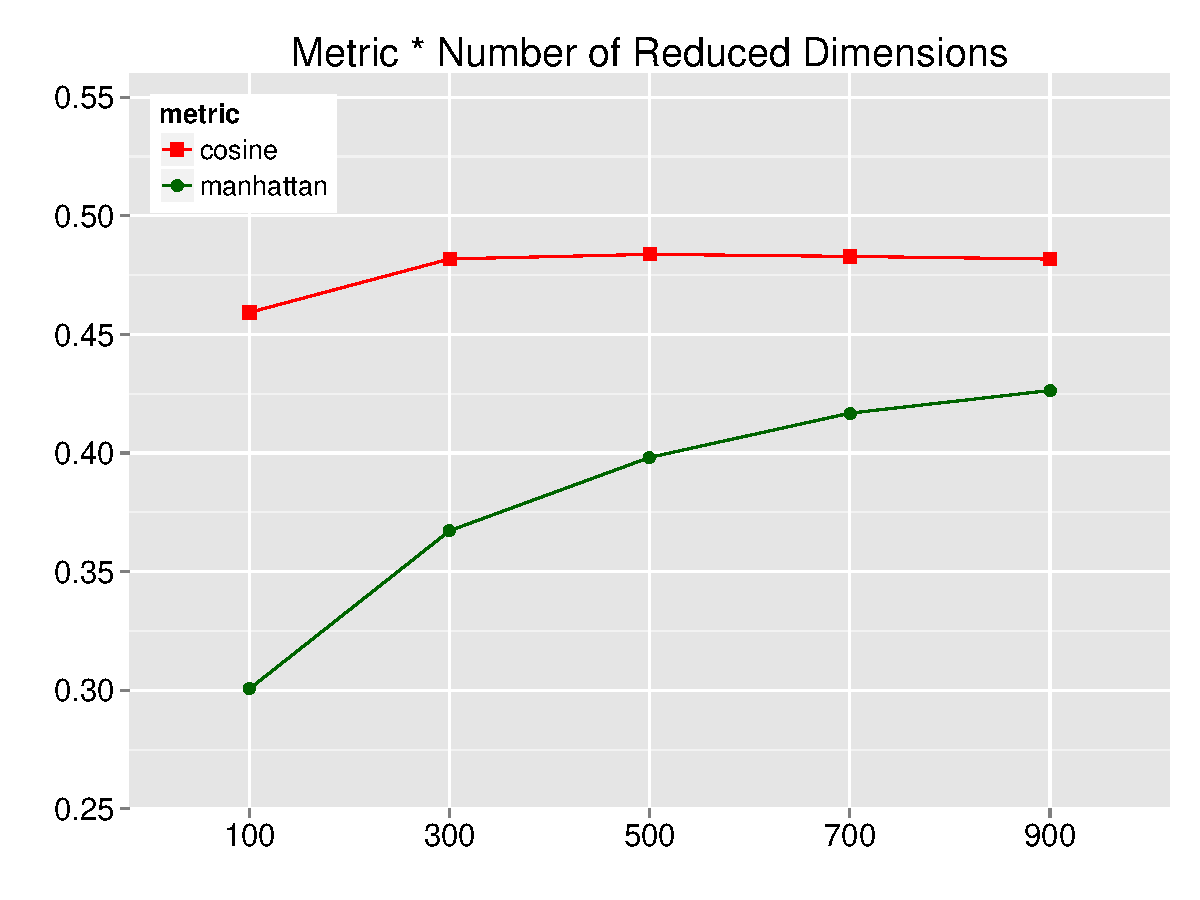
\includegraphics[scale=0.30]{img/lapesa_ws_main_metric_n-dim}
        \vspace{-10pt}
        \caption{WordSim353 dataset}
      \end{figure}
      
    \end{column}
  \end{columns}  
  
\end{frame}



\begin{frame}
  \frametitle{Correlation to Ratings: Partial Effects}
  \framesubtitle{Quite Explanatory Parameters: Number of Skipped Dimensions}

  \vspace{-18pt}

  \begin{columns}
    
    \begin{column}{0.5\textwidth}
      \begin{figure} 
        \hspace*{-18pt} 
        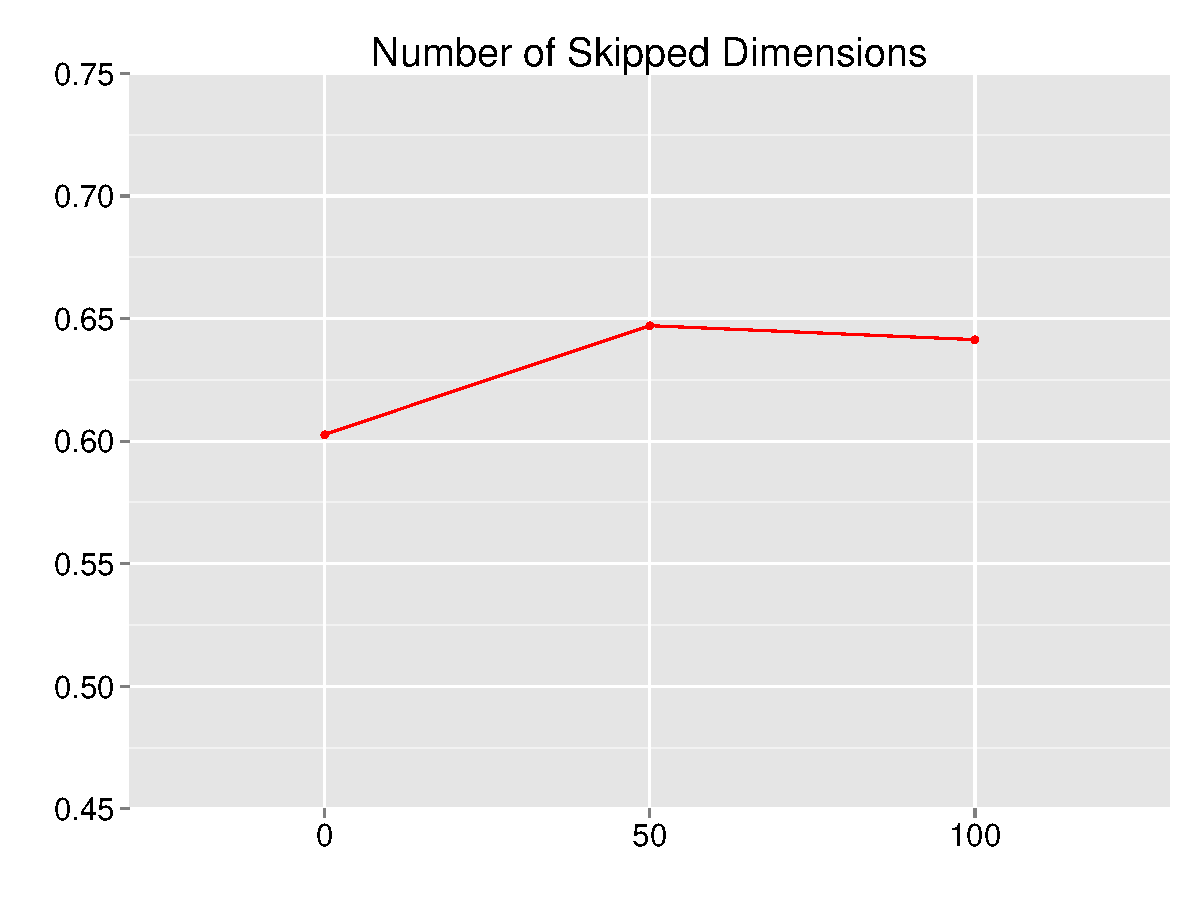
\includegraphics[scale=0.30]{img/lapesa_rg_main_dimskip}
        \vspace{-10pt}
        \caption{Rubenstein Goodenough dataset}
      \end{figure}
    \end{column}

    \begin{column}{0.5\textwidth}
      \centering
      
      \begin{figure}
        \hspace*{-18pt}   
        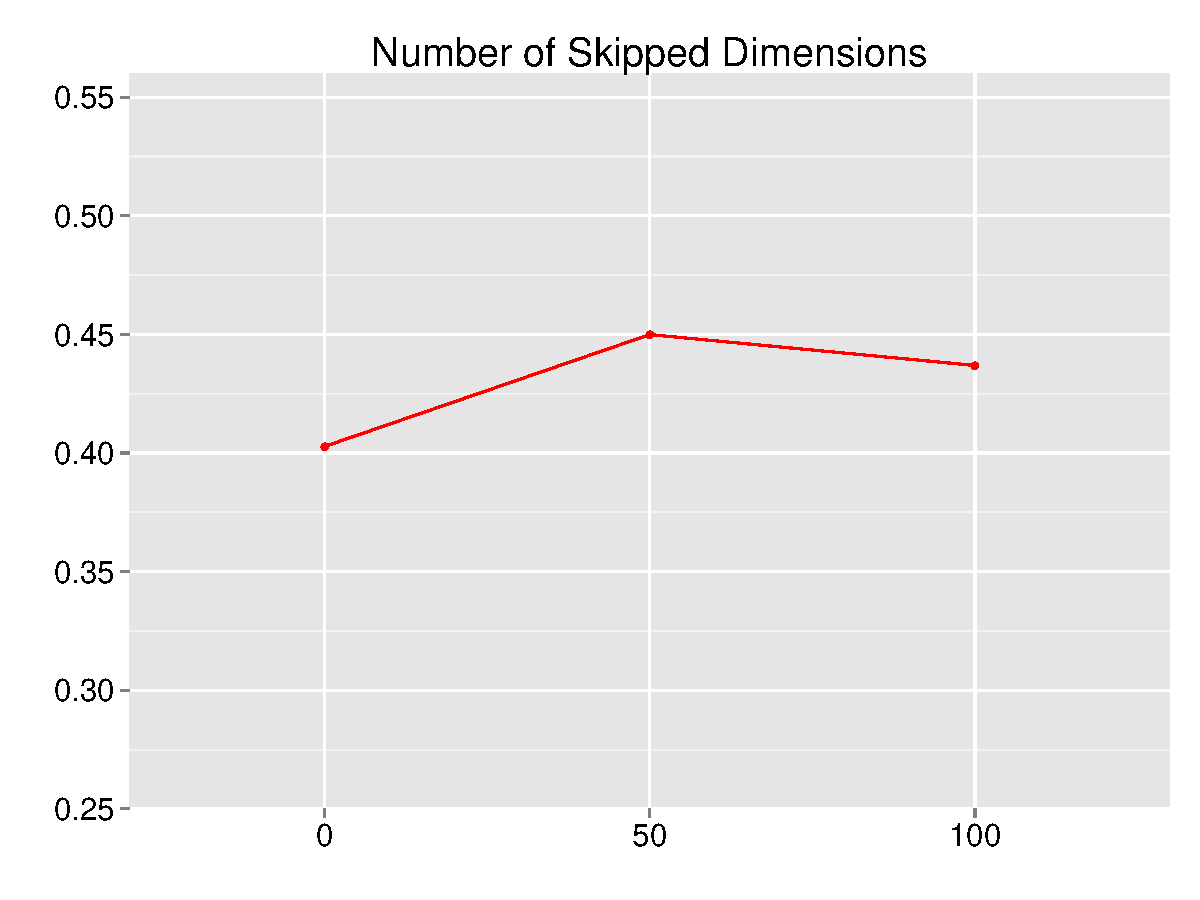
\includegraphics[scale=0.30]{img/lapesa_ws_main_dimskip}
        \vspace{-10pt}
        \caption{WordSim353 dataset}
      \end{figure}
      
    \end{column}
  \end{columns}  
  
\end{frame}

\begin{frame}
  \frametitle{Correlation to Ratings: Partial Effects}
  \framesubtitle{Quite Explanatory Parameters: Window * Transformation}

  \vspace{-18pt}

  \begin{columns}
    
    \begin{column}{0.5\textwidth}
      \begin{figure} 
        \hspace*{-18pt} 
        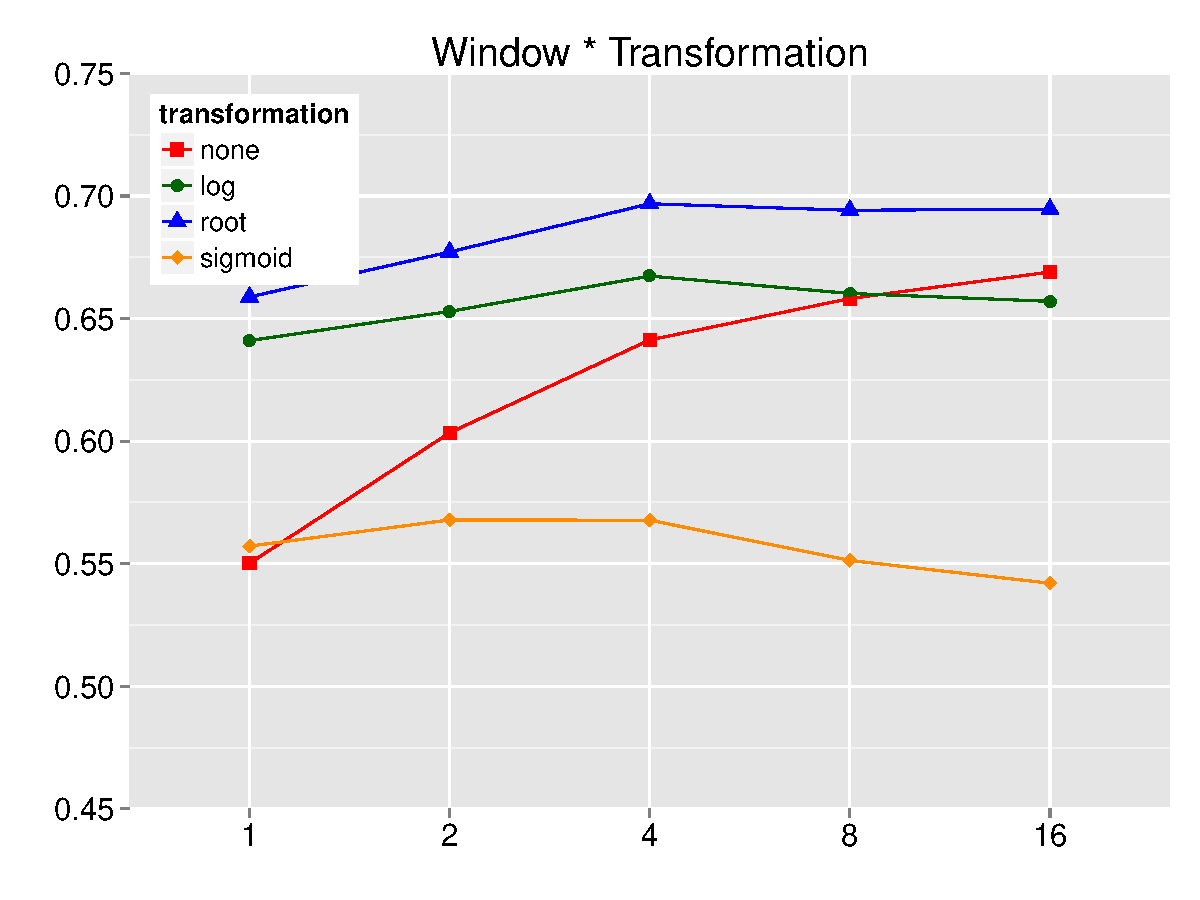
\includegraphics[scale=0.30]{img/lapesa_rg_main_window_transformation}
        \vspace{-10pt}
        \caption{Rubenstein Goodenough dataset}
      \end{figure}
    \end{column}

    \begin{column}{0.5\textwidth}
      \centering
      
      \begin{figure}
        \hspace*{-18pt}   
        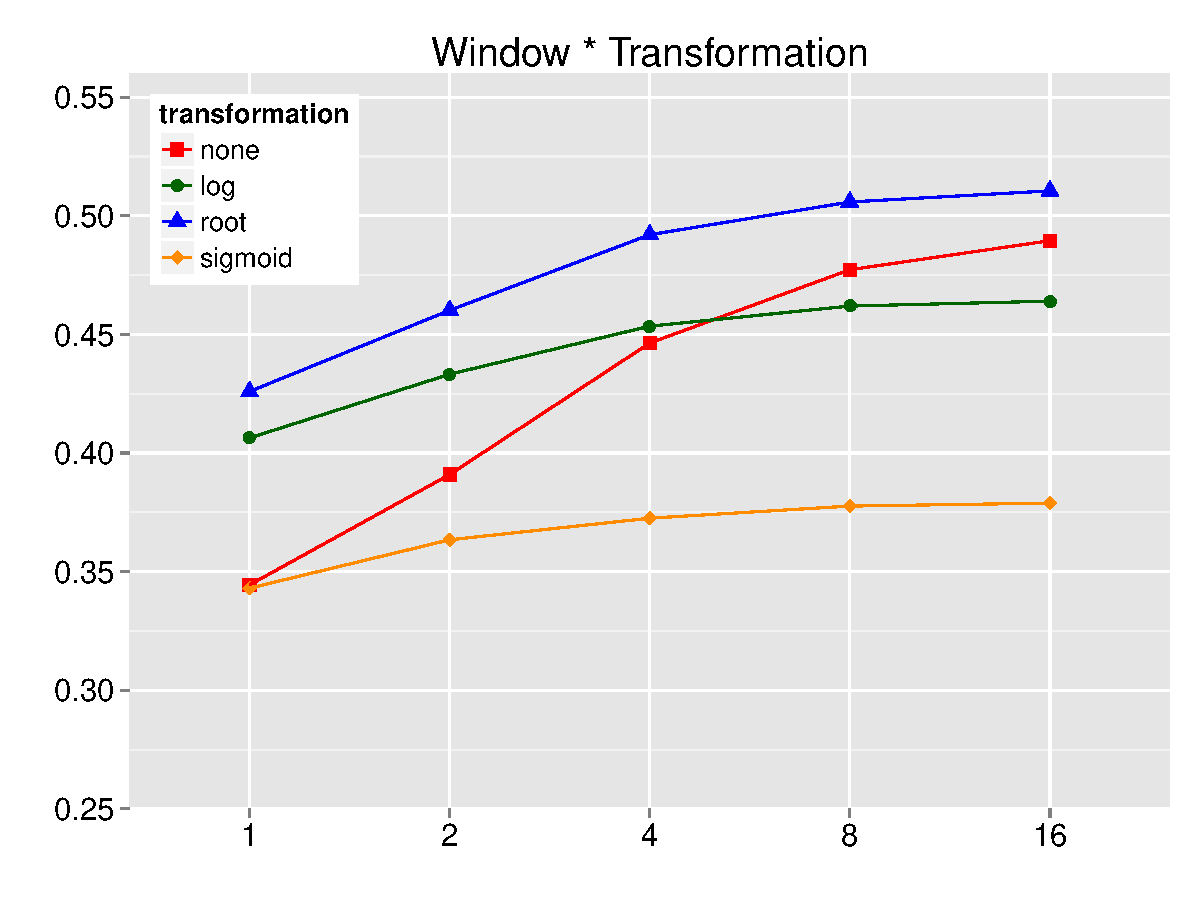
\includegraphics[scale=0.30]{img/lapesa_ws_main_window_transformation}
        \vspace{-10pt}
        \caption{WordSim353 dataset}
      \end{figure}
      
    \end{column}
  \end{columns}  
  
\end{frame}




\begin{frame}
  \frametitle{Summing up: Ratings}
  \begin{exampleblock}{Ratings: best setting}
    \begin{itemize}\footnotesize
    \item Corpus: wacky
    \item Window: undirected, 4 words 
    \item Feature selection: top 20000/50000 dimensions, based on frequency
    \item Score * Transformation: simple-ll * log
    \item Dimensionality Reduction: 300 latent dimensions, skipping the first 50
    \item Distance Metric: cosine
    \item Index of Distributional Relatedness: neighbor rank
    \end{itemize}
  \end{exampleblock}   
  
\end{frame}


\begin{frame}
  \frametitle{DSMs and Semantic Clustering}
  \framesubtitle{Introducing the task: the datasets}

  \ungap[1.5]
  \begin{columns}
    \begin{column}{0.5 \textwidth}
      \begin{exampleblock}{Almuhareb Poesio}
        \textbf{402 nouns, 21 classes} \\
        \textit{day} $\Longrightarrow$ \textsc{TIME}   \\
        \textit{kiwi} $\Longrightarrow$ \textsc{FRUIT}  \\
        \textit{kitten} $\Longrightarrow$ \textsc{ANIMAL} \\
        \textit{volleyball} $\Longrightarrow$ \textsc{GAME}
      \end{exampleblock}
      \begin{exampleblock}{ESSLLI categorization task}
        \textbf{44 nouns, 6 classes} \\
        \textit{potato} $\Longrightarrow$ \textsc{GREEN}  \\
        \textit{hammer} $\Longrightarrow$ \textsc{TOOL}  \\
        \textit{car} $\Longrightarrow$ \textsc{VEHICLE} \\
        \textit{peacock} $\Longrightarrow$ \textsc{BIRD}     
      \end{exampleblock}
    \end{column}
    \begin{column}{0.5 \textwidth}
      \begin{exampleblock}{BATTIG set}
        \textbf{83 nouns, 10 classes} \\
        \textit{chicken} $\Longrightarrow$ \textsc{BIRD}   \\
        \textit{bear} $\Longrightarrow$ \textsc{LAND\_MAMMAL}  \\
        \textit{pot} $\Longrightarrow$ \textsc{KITCHENWARE} \\
        \textit{oak} $\Longrightarrow$ \textsc{TREE} 
      \end{exampleblock}
      \begin{exampleblock}{MITCHELL set}
        \textbf{60 nouns, 12 classes} \\
        \textit{ant} $\Longrightarrow$ \textsc{INSECT}   \\
        \textit{carrot} $\Longrightarrow$ \textsc{VEGETABLE}  \\
        \textit{train} $\Longrightarrow$ \textsc{VEHICLE} \\
        \textit{cat} $\Longrightarrow$ \textsc{ANIMAL}
      \end{exampleblock}
    \end{column}
  \end{columns}
\end{frame}

\begin{frame}
  \frametitle{DSMs and Semantic Clustering}
  \framesubtitle{Introducing the task}

  \begin{itemize}
  \item A \textbf{categorization} task
  \item If distributional representations approximate human conceptual representations, we expect word categorization based on distributional features to produce concept clusters similar to those in the gold standard datasets
  \item Performance: \textbf{cluster purity}
    \begin{itemize}
    \item classification accuracy for optimal cluster labelling
    \item percentage of nouns that belong to the majority category within their cluster 
    \end{itemize}
  \end{itemize}
\end{frame}


\begin{frame}
  \frametitle{Semantic Clustering: Performance}
  \framesubtitle{Overview: Unreduced versus Reduced Experiments}

  \begin{center}
    \begin{tabular}{|l|c|c|c|c|c|c|}
      \hline
      \multirow{2}{*}{Dataset}  & \multicolumn{3}{c|}{Unreduced} &  \multicolumn{3}{c|}{Reduced} \\  \cline{2-7}
      & Min & Max & Mean & Min & Max & Mean \\ \hline
      
      AP & 0.15 & 0.73 & 0.56 & 0.13 & \primary{0.76} & 0.54 \\  
      BATTIG & 0.28 & \primary{0.99} & 0.77 & 0.23 & \primary{0.99} & 0.78  \\  
      ESSLLI & 0.32 & 0.93 & 0.72 & 0.32 & \primary{0.98} & 0.72  \\    
      MITCHELL & 0.26 & \primary{0.97} & 0.68 & 0.27 & \primary{0.97} & 0.69 \\    \hline
      
    \end{tabular}

    \gap[1]
    \secondary{Semantic Clustering: summary of performance (purity)} 
  \end{center}
  
\end{frame}

\begin{frame}
  \frametitle{Semantic Clustering: Parameters and Explained Variance}
  \framesubtitle{Feature Ablation  (model $R^{2}$ - AP: 82\%;  BATTIG: 77\% ; ESSLLI  58\%; MITCHELL 73\%)}
  \centering
  \hspace*{-10pt}
  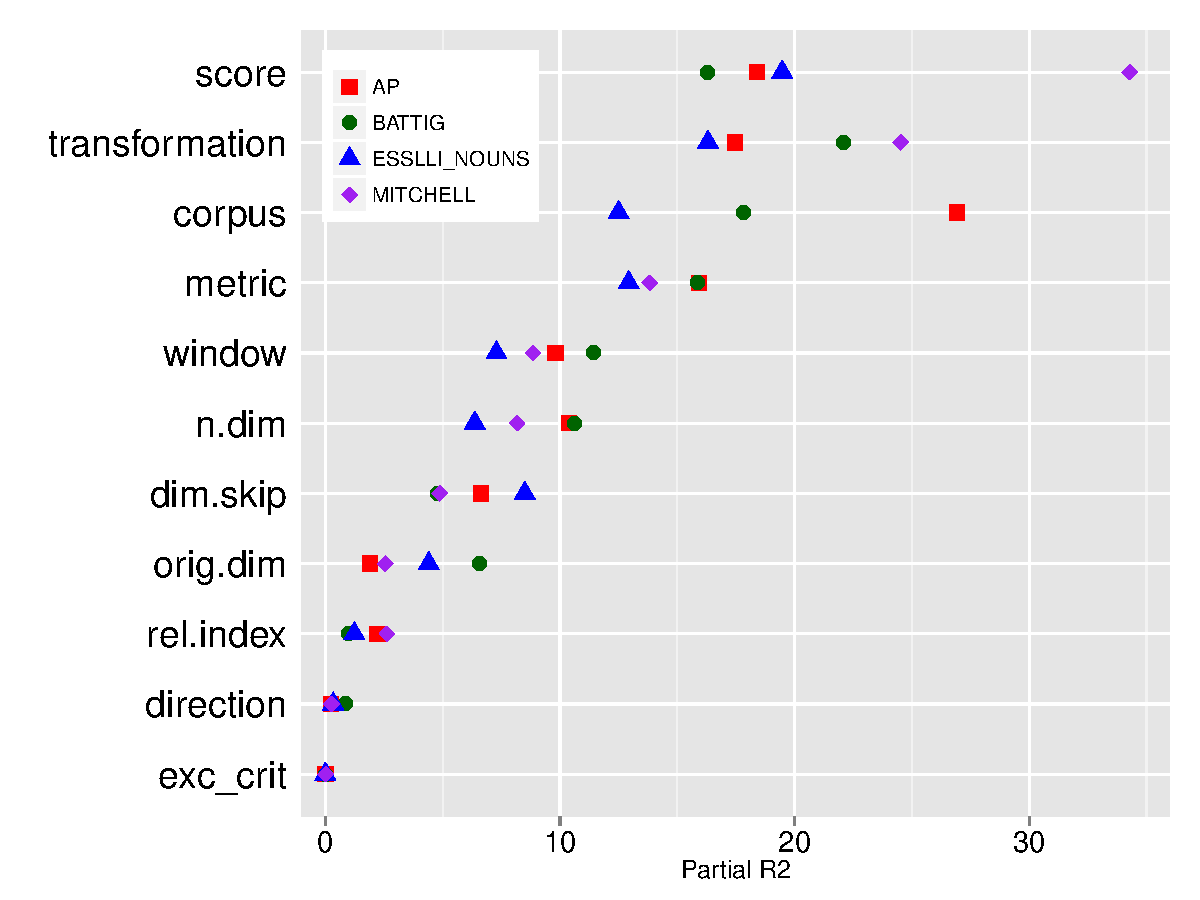
\includegraphics[scale=0.45]{img/lapesa_clustering_main_r2_reduced}

\end{frame}

\begin{frame}
  \frametitle{Semantic Clustering: Interactions and Explained Variance}
  \framesubtitle{Reduced setting ($R^{2}$ $>$ 0.5 )}
  
  \begin{center}\small
    \begin{tabular}{lrrrrr}
      
      Interaction & Df & AP & BATTIG & ESSLLI & MITCHELL \\ \hline
      
      \primary{score:transformation} & 18 &  7.10  & 7.95 & 7.56  &  11.42   \\ 
      \primary{window:metric} & 4 &  2.22   & 1.26 & 2.97  & 2.72    \\
      \primary{metric:n.dim} & 4 &   3.29    & 3.16 &  2.03 &  0.58   \\   
      \primary{metric:dim.skip} & 2 &   2.25   & 1.54 & 2.77  & 	 0.86  \\   
      \primary{window:transformation} & 12 &  2.00  & 2.95 & 0.88  &   2.66 \\ 


      corpus:metric & 2 &  1.42  & 2.91 & 2.79   & 1.11      \\ 
      corpus:window & 8 &   2.36   & 1.18 & 1.49  &    1.23   \\ 
      score:dim.skip & 12 &  0.56 & 1.15 &   0.99 &   1.39 \\ 
      window:score & 24 &  0.74   & 0.77 &  0.54  &  0.65  \\  
      %% metric:orig.dim & 4 &    -  & 1.20 &  0.67  &  0.92  \\ 
      %% transformation:dim.skip & 6 &   -   & 1.17 &  0.85  &  1.39    \\   
    \end{tabular}

    \gap[1]
    \secondary{Clustering datasets: interactions, $R^2$} 
  \end{center}
  
\end{frame}


\begin{frame}
  \frametitle{Semantic Clustering: Partial Effects}
  \framesubtitle{Most Explanatory Parameters: Score * Transformation}

  \vspace{-18pt}

  \begin{columns}
    
    \begin{column}{0.5\textwidth}
      \begin{figure} 
        \hspace*{-18pt} 
        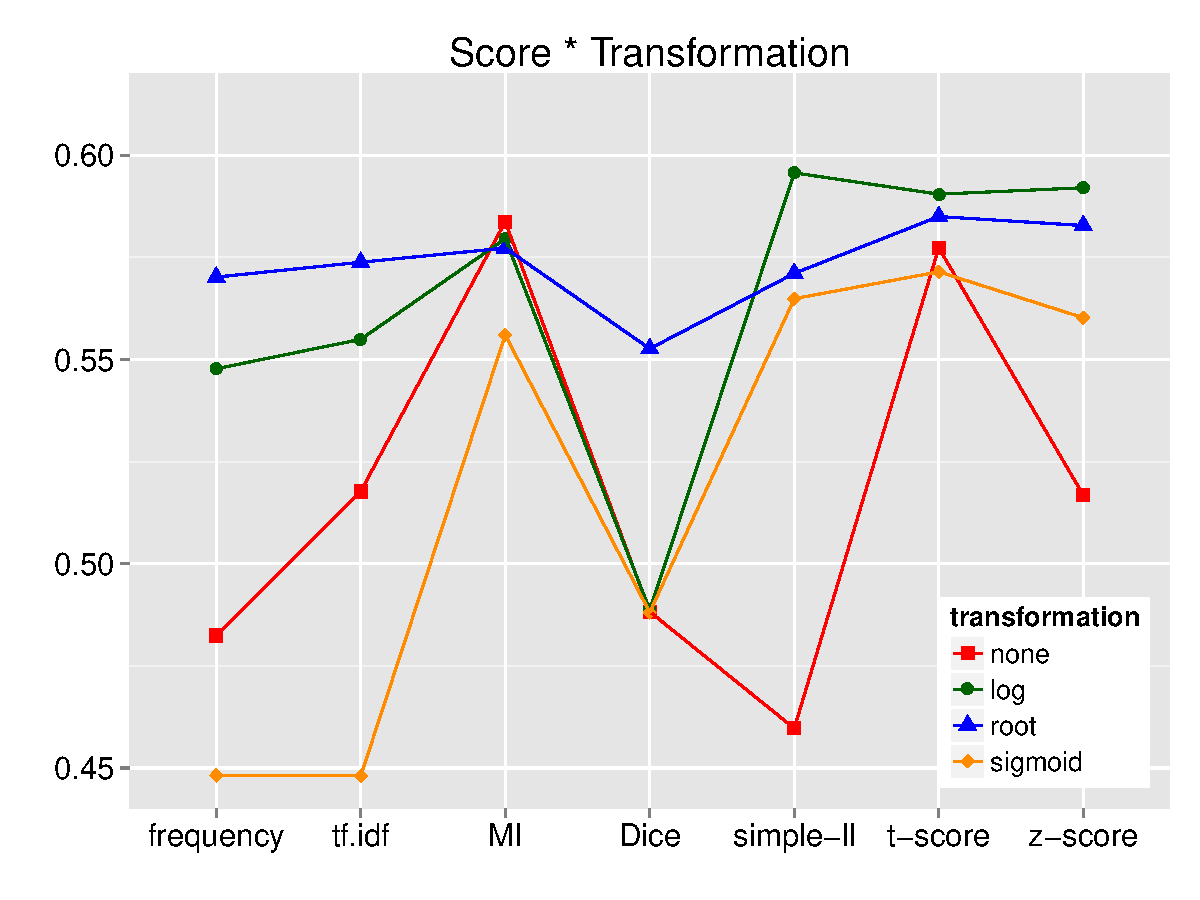
\includegraphics[scale=0.30]{img/lapesa_ap_main_score_transformation}
        \vspace{-10pt}
        \caption{AP dataset}
      \end{figure}
    \end{column}

    \begin{column}{0.5\textwidth}
      \centering
      
      \begin{figure}
        \hspace*{-18pt}   
        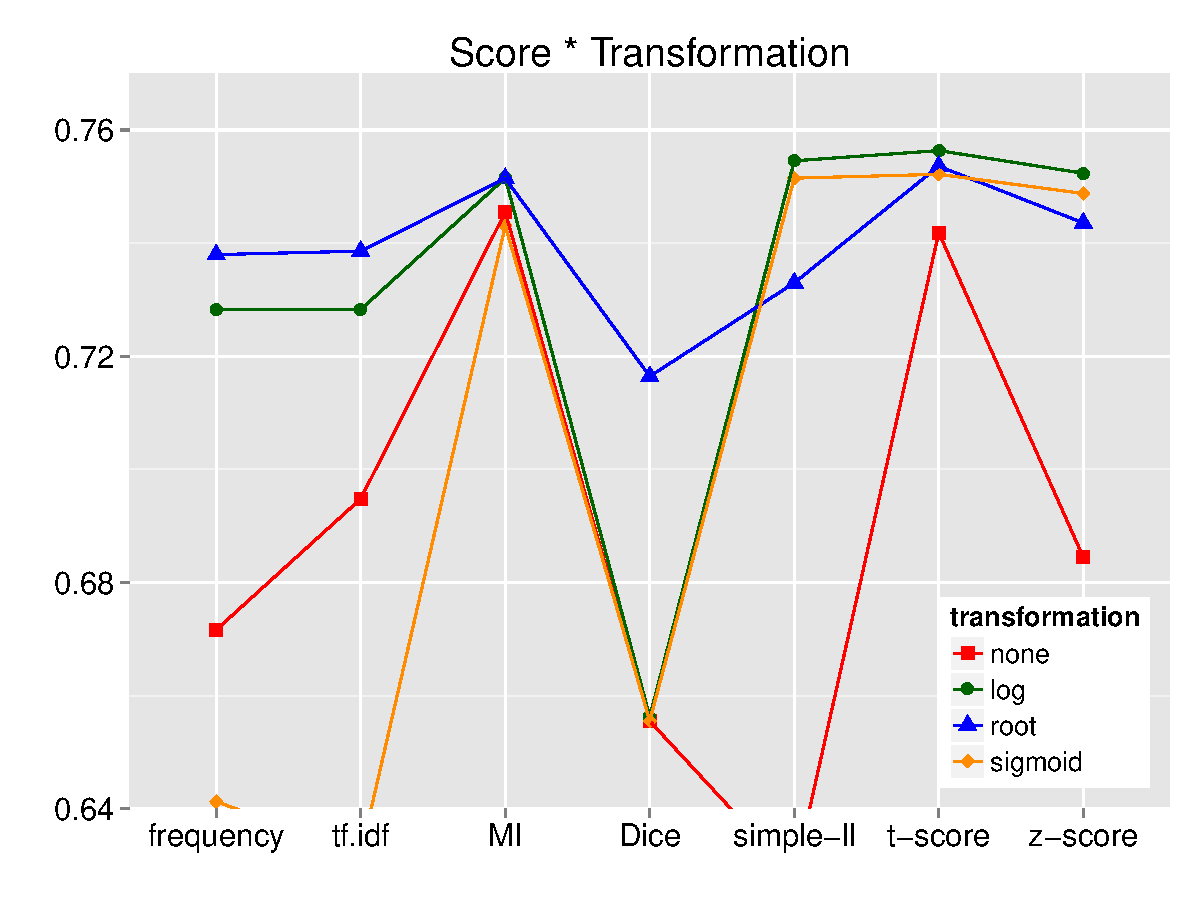
\includegraphics[scale=0.30]{img/lapesa_esslli_main_score_transformation}
        \vspace{-10pt}
        \caption{ESSLLI dataset}
      \end{figure}
      
    \end{column}
  \end{columns}  
  
\end{frame}

\begin{frame}
  \frametitle{Semantic Clustering: Partial Effects}
  \framesubtitle{Most Explanatory Parameters: Corpus}

  \vspace{-18pt}

  \begin{columns}
    
    \begin{column}{0.5\textwidth}
      \begin{figure} 
        \hspace*{-18pt} 
        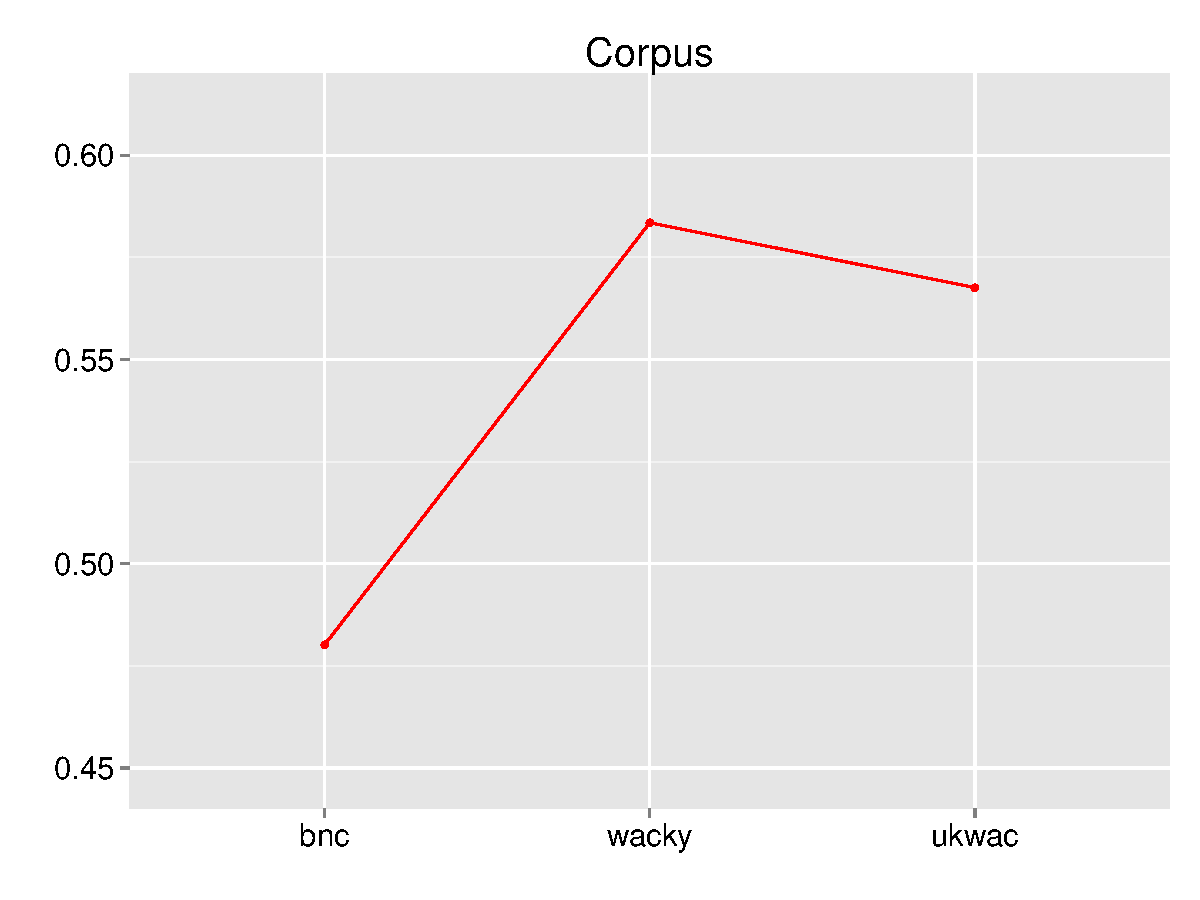
\includegraphics[scale=0.30]{img/lapesa_ap_main_corpus}
        \vspace{-10pt}
        \caption{AP dataset}
      \end{figure}
    \end{column}

    \begin{column}{0.5\textwidth}
      \centering
      
      \begin{figure}
        \hspace*{-18pt}   
        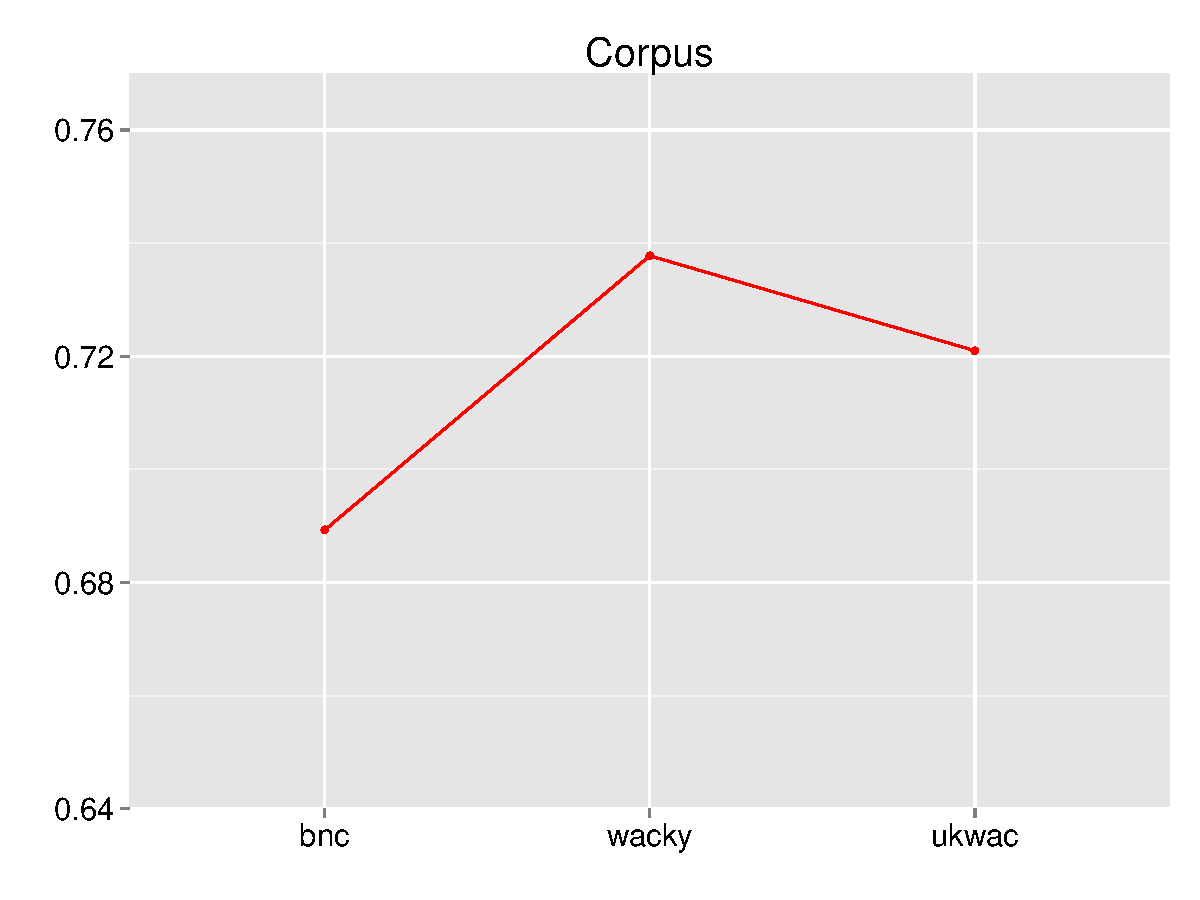
\includegraphics[scale=0.30]{img/lapesa_esslli_main_corpus}
        \vspace{-10pt}
        \caption{ESSLLI dataset}
      \end{figure}
      
    \end{column}
  \end{columns}  
  
\end{frame}



\begin{frame}
  \frametitle{Semantic Clustering: Partial Effects}
  \framesubtitle{Most Explanatory Parameters: Window * Metric}
  
  \vspace{-18pt}   

  \begin{columns}
    
    \begin{column}{0.5\textwidth}
      \begin{figure} 
        \hspace*{-18pt} 
        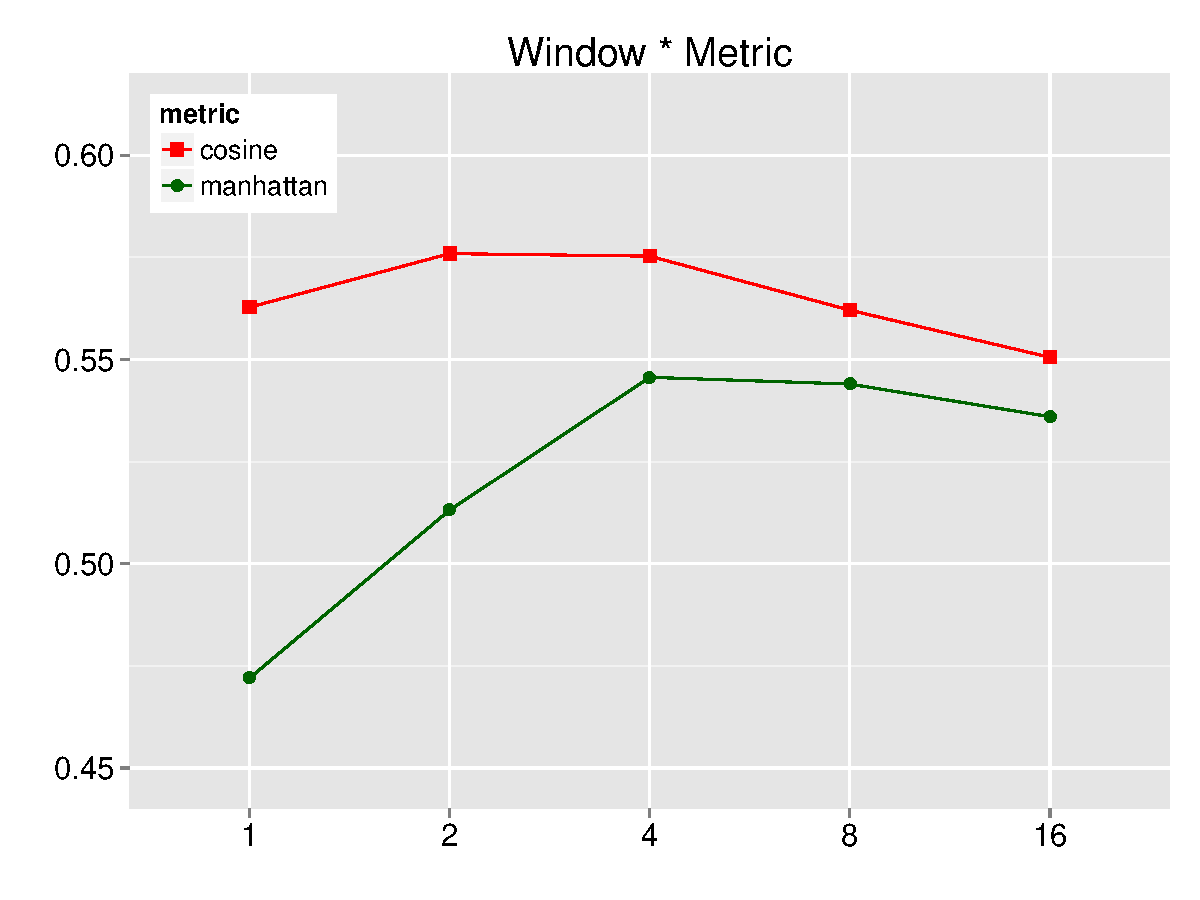
\includegraphics[scale=0.30]{img/lapesa_ap_main_window_metric}
        \vspace{-10pt}
        \caption{AP dataset}
      \end{figure}
    \end{column}

    \begin{column}{0.5\textwidth}
      \centering
      
      \begin{figure}
        \hspace*{-18pt}   
        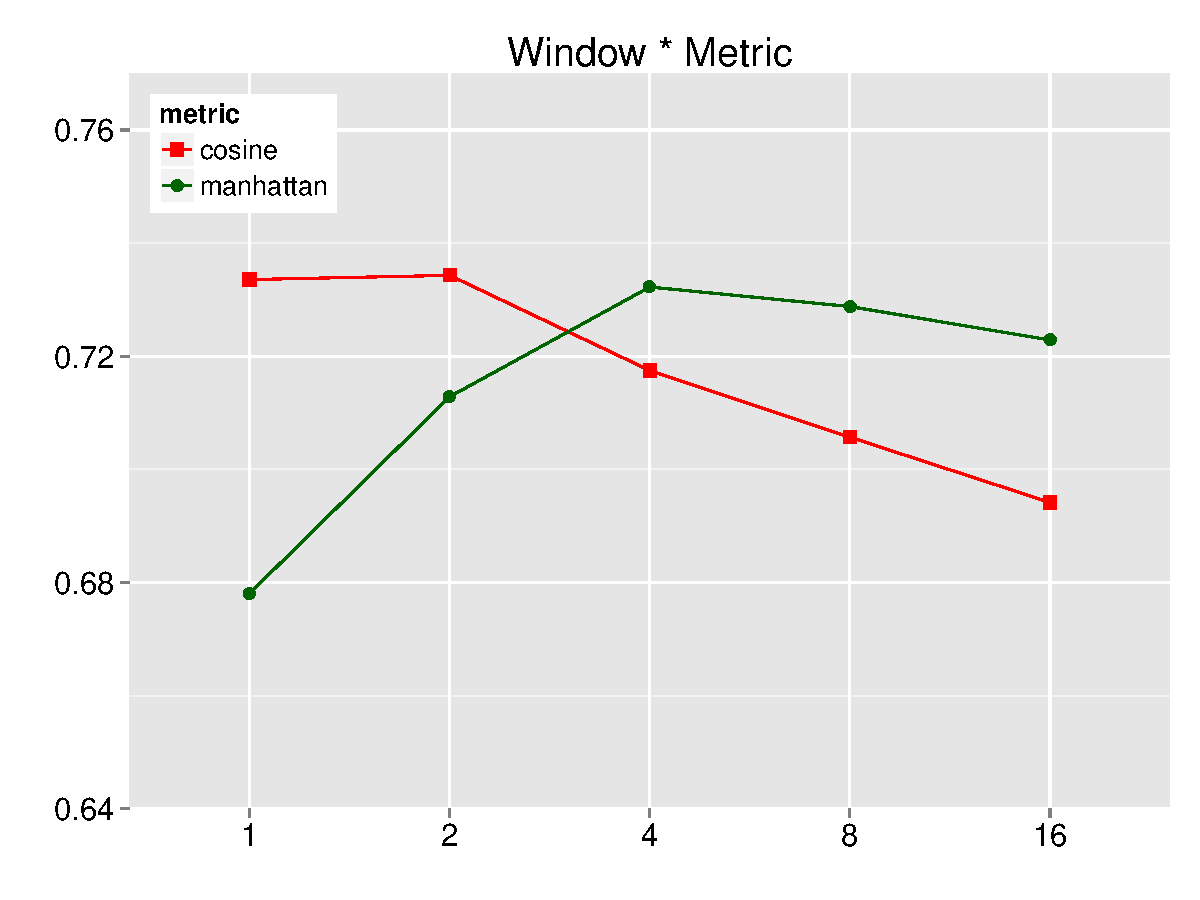
\includegraphics[scale=0.30]{img/lapesa_esslli_main_window_metric}
        \vspace{-10pt}
        \caption{ESSLLI dataset}
      \end{figure}
      
    \end{column}
  \end{columns}  
  
\end{frame}


\begin{frame}
  \frametitle{Semantic Clustering: Partial Effects}
  \framesubtitle{Quite Explanatory Parameters: Metric * Number of Reduced Dimensions}
  
  \vspace{-18pt}   

  \begin{columns}
    
    \begin{column}{0.5\textwidth}
      \begin{figure} 
        \hspace*{-18pt} 
        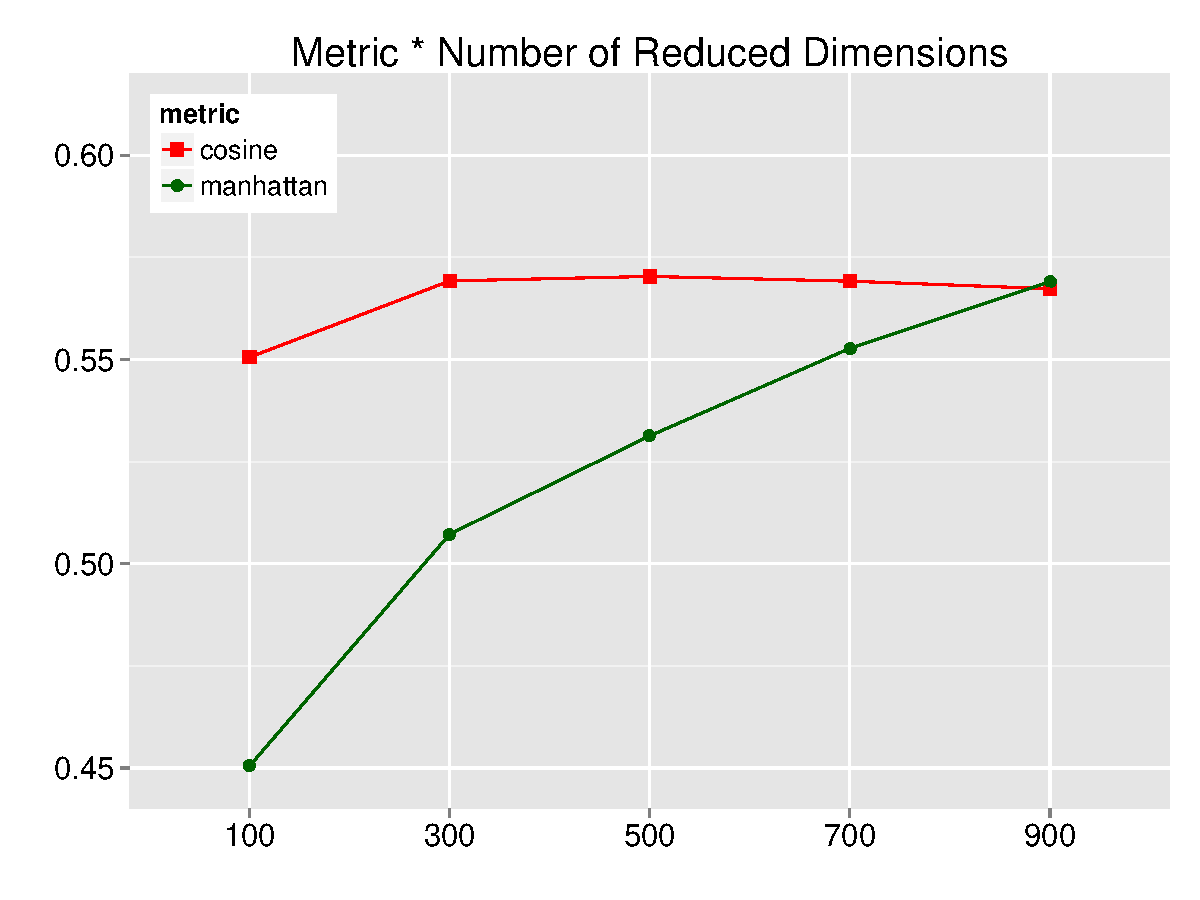
\includegraphics[scale=0.30]{img/lapesa_ap_main_metric_n-dim}
        \vspace{-10pt}
        \caption{AP dataset}
      \end{figure}
    \end{column}

    \begin{column}{0.5\textwidth}
      \centering
      
      \begin{figure}
        \hspace*{-18pt}   
        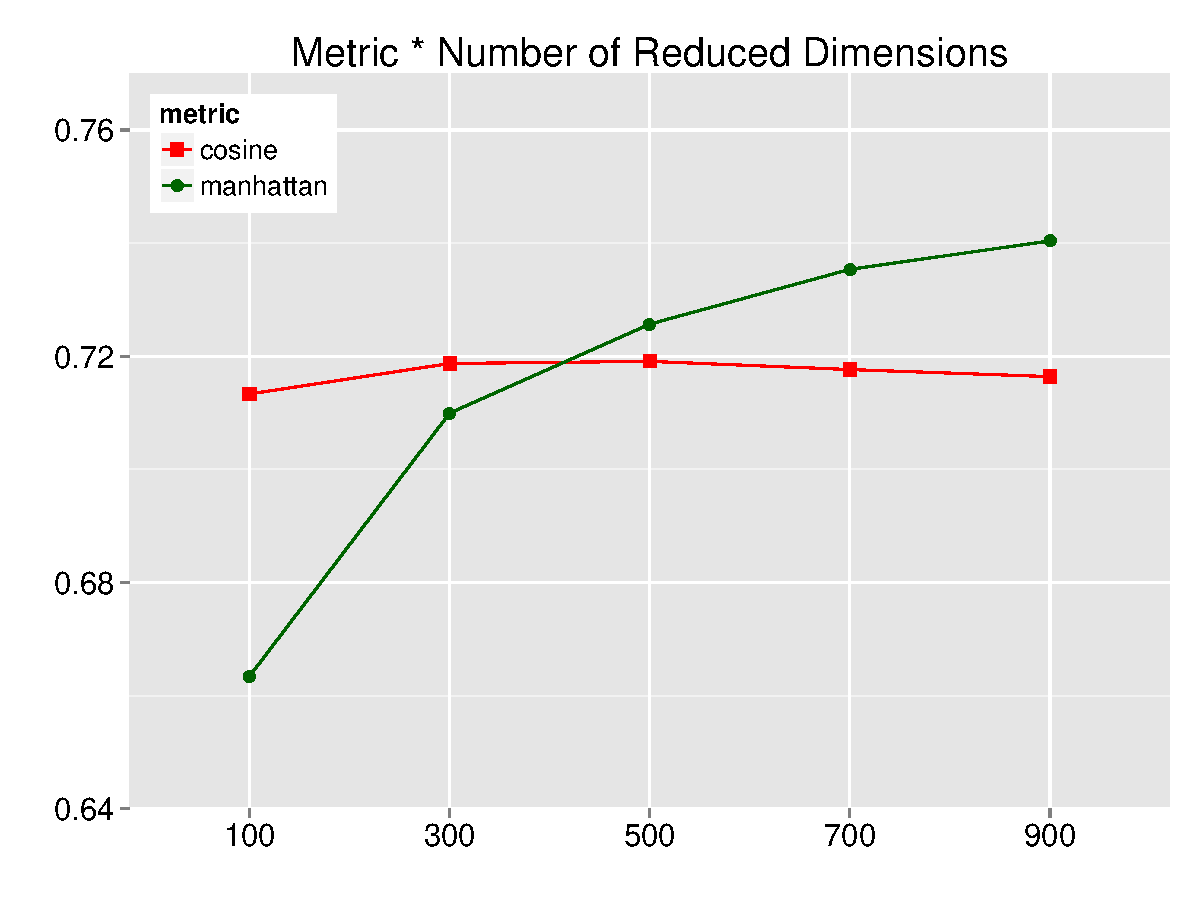
\includegraphics[scale=0.30]{img/lapesa_esslli_main_metric_n-dim}
        \vspace{-10pt}
        \caption{ESSLLI dataset}
      \end{figure}
      
    \end{column}
  \end{columns}  
  
\end{frame}

\begin{frame}
  \frametitle{Semantic Clustering: Partial Effects}
  \framesubtitle{Quite Explanatory Parameters: Number of skipped dimensions}

  \vspace{-18pt}

  \begin{columns}
    
    \begin{column}{0.5\textwidth}
      \begin{figure} 
        \hspace*{-18pt} 
        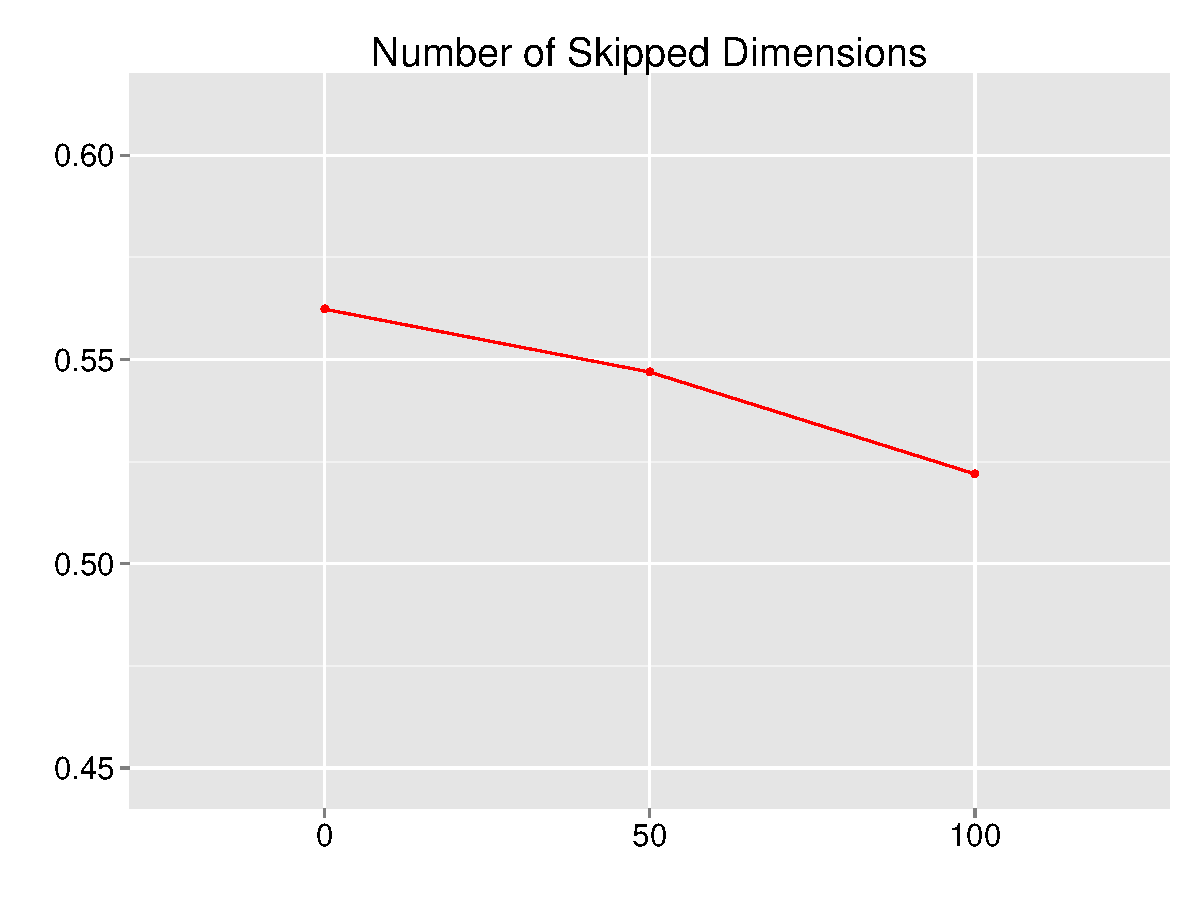
\includegraphics[scale=0.30]{img/lapesa_ap_main_dimskip}
        \vspace{-10pt}
        \caption{AP dataset}
      \end{figure}
    \end{column}

    \begin{column}{0.5\textwidth}
      \centering
      
      \begin{figure}
        \hspace*{-18pt}   
        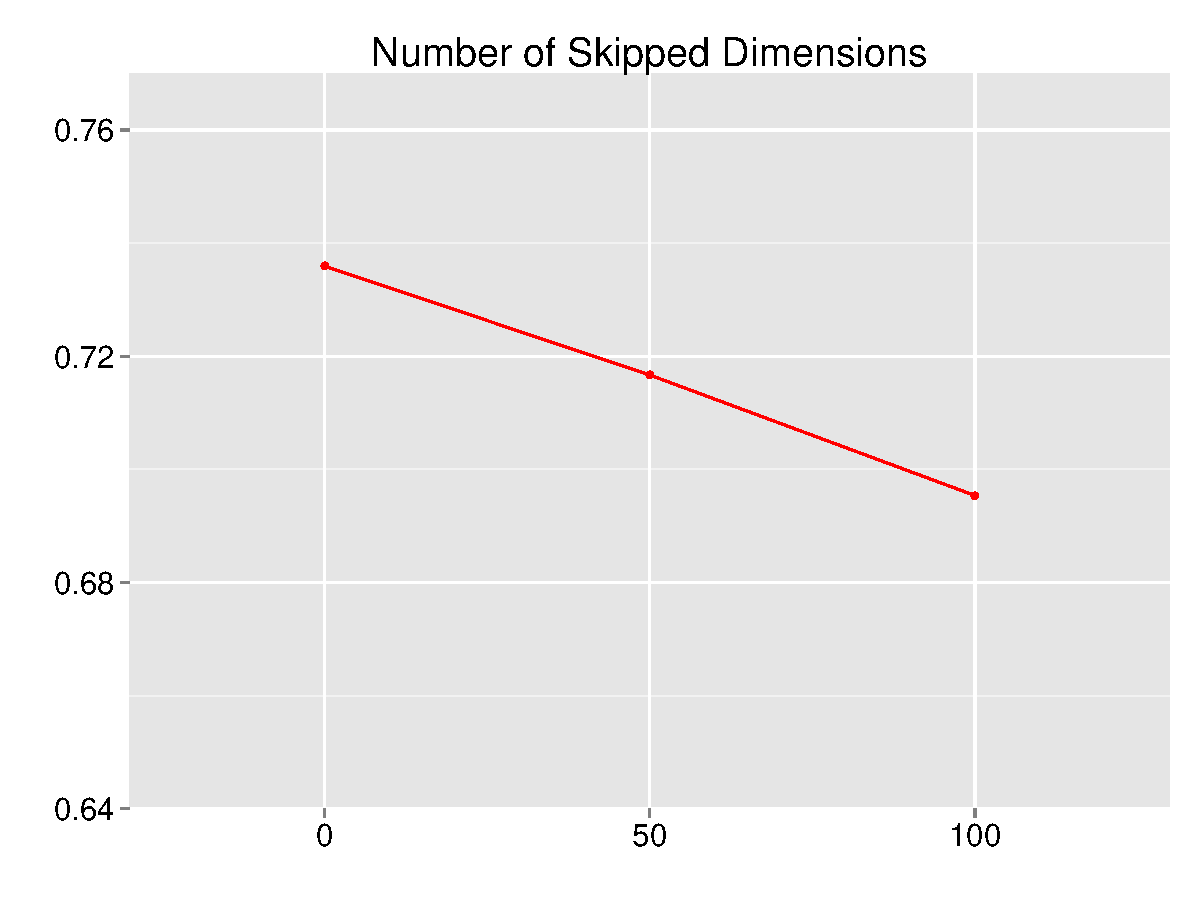
\includegraphics[scale=0.30]{img/lapesa_esslli_main_dimskip}
        \vspace{-10pt}
        \caption{ESSLLI dataset}
      \end{figure}
      
    \end{column}
  \end{columns}  
  
\end{frame}




\begin{frame}
  \frametitle{Semantic Clustering: Partial Effects}
  \framesubtitle{Less explanatory parameters: Relatedness Index}

  \vspace{-18pt}

  \begin{columns}
    
    \begin{column}{0.5\textwidth}
      \begin{figure} 
        \hspace*{-18pt} 
        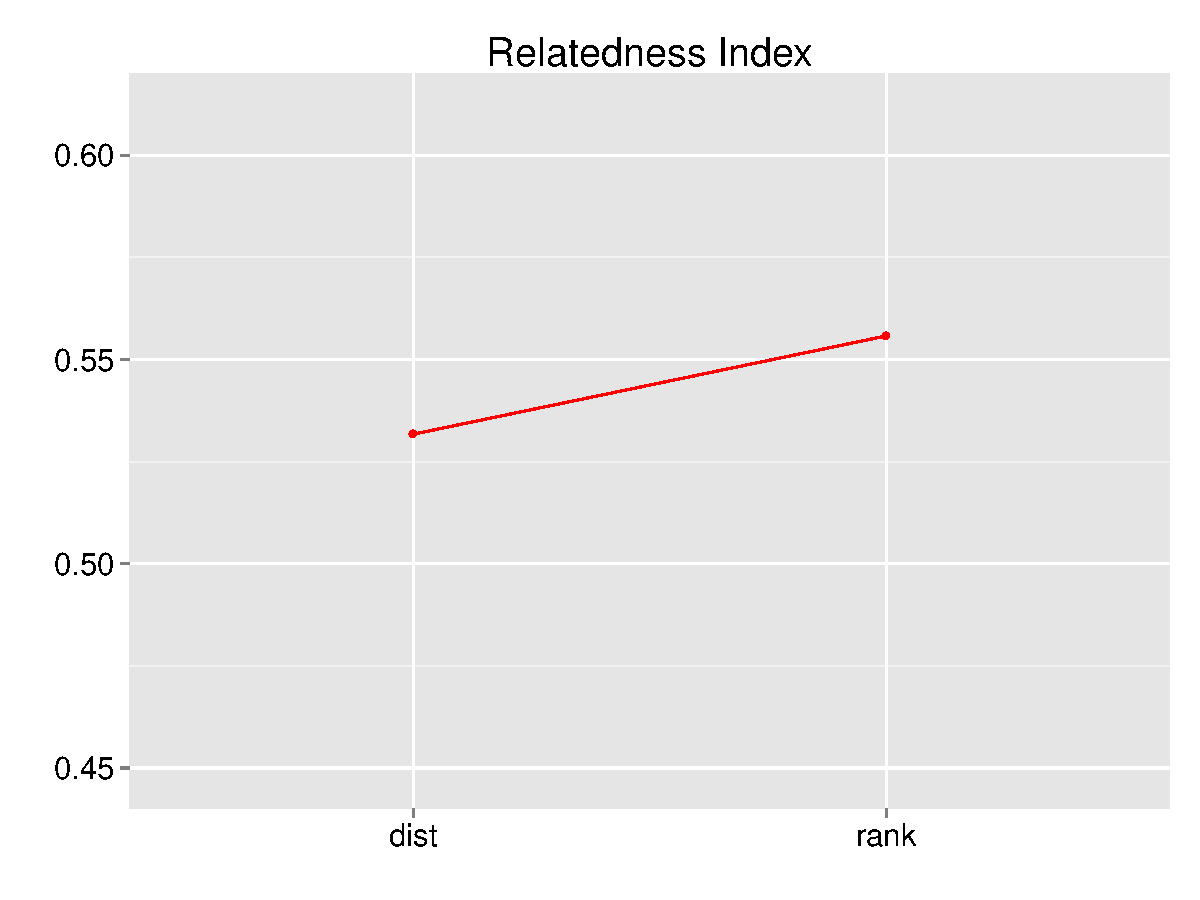
\includegraphics[scale=0.30]{img/lapesa_ap_main_relindex}
        \vspace{-10pt}
        \caption{AP dataset}
      \end{figure}
    \end{column}

    \begin{column}{0.5\textwidth}
      \centering
      
      \begin{figure}
        \hspace*{-18pt}   
        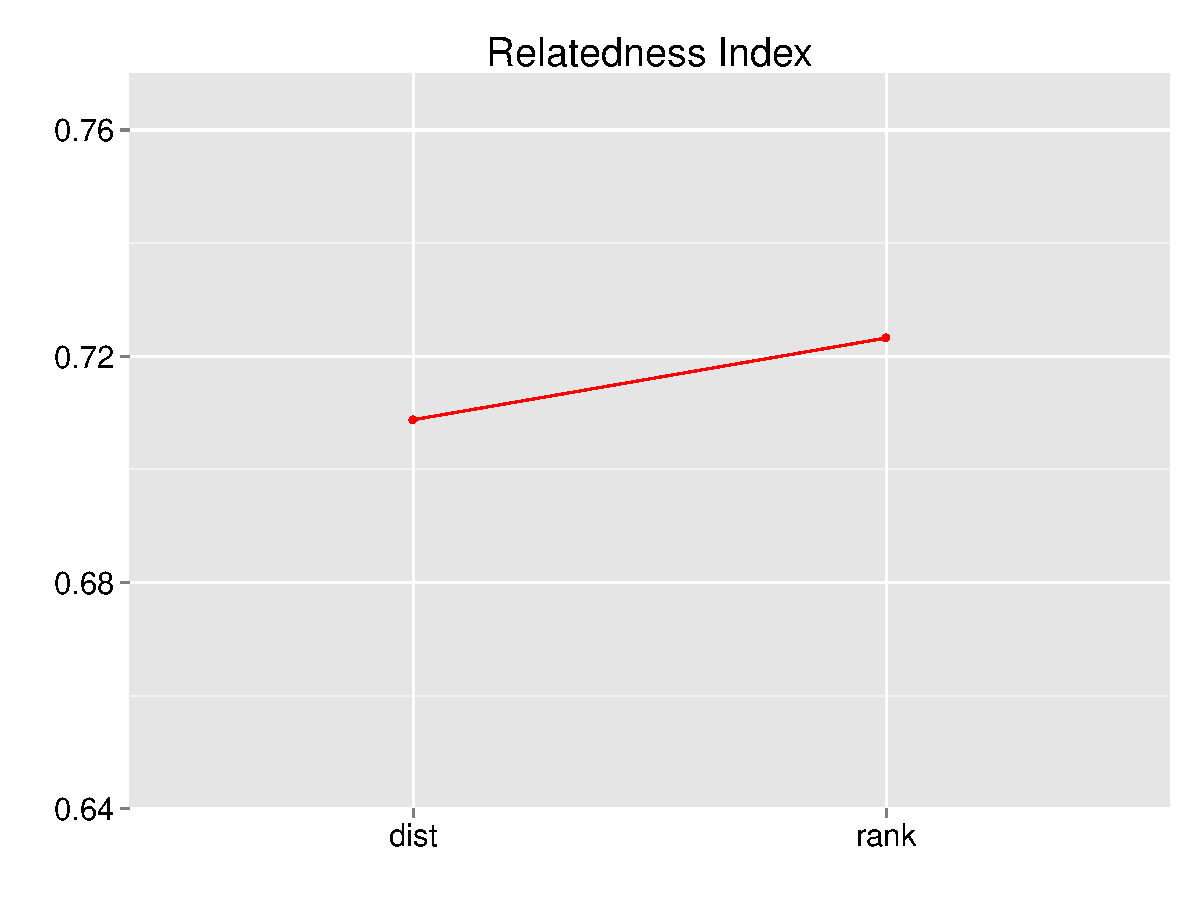
\includegraphics[scale=0.30]{img/lapesa_esslli_main_relindex}
        \vspace{-10pt}
        \caption{ESSLLI dataset}
      \end{figure}
      
    \end{column}
  \end{columns}  
  
\end{frame}

\begin{frame}
  \frametitle{Semantic Clustering: Partial Effects}
  \framesubtitle{Less explanatory parameters: Number of original dimensions}

  \vspace{-18pt}

  \begin{columns}
    
    \begin{column}{0.5\textwidth}
      \begin{figure} 
        \hspace*{-18pt} 
        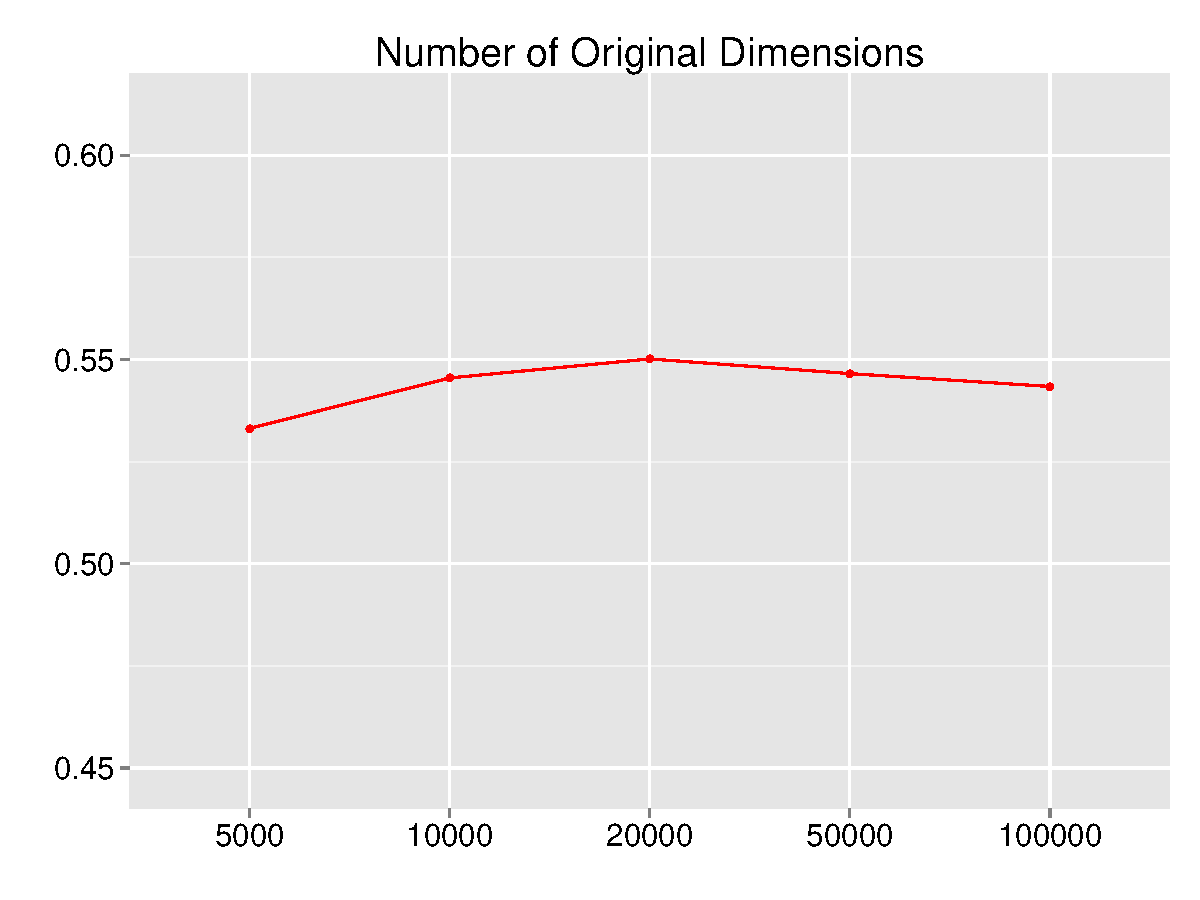
\includegraphics[scale=0.30]{img/lapesa_ap_main_origdim}
        \vspace{-10pt}
        \caption{AP dataset}
      \end{figure}
    \end{column}

    \begin{column}{0.5\textwidth}
      \centering
      
      \begin{figure}
        \hspace*{-18pt}   
        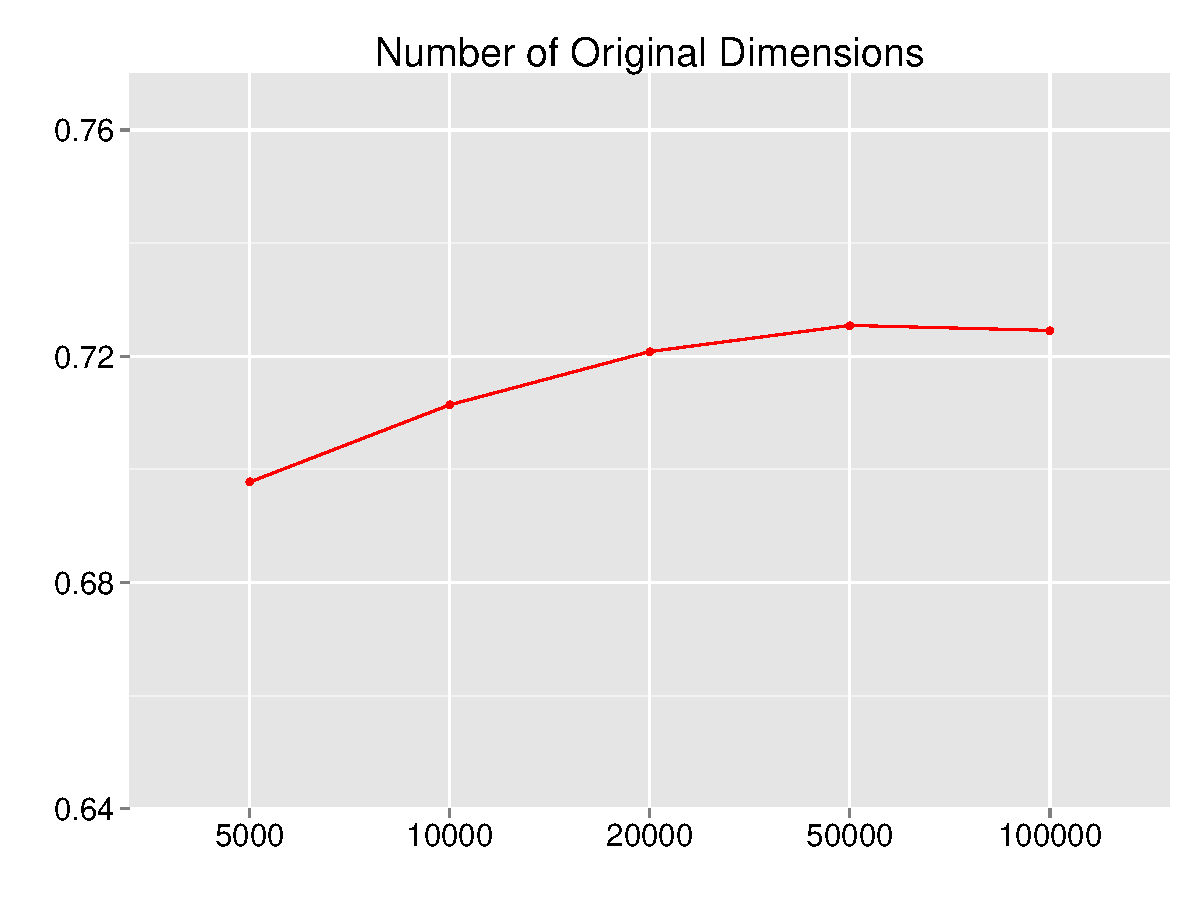
\includegraphics[scale=0.30]{img/lapesa_esslli_main_origdim}
        \vspace{-10pt}
        \caption{ESSLLI dataset}
      \end{figure}
      
    \end{column}
  \end{columns}  
  
\end{frame}


\begin{frame}
  \frametitle{Summing up: Semantic Clustering}
  \begin{exampleblock}{Clustering: best setting}
    \begin{itemize}
    \item Corpus: wacky
    \item Window: undirected, 4 words 
    \item Feature selection: top 50000 dimensions, based on frequency
    \item Score * Transformation: simple-ll * log (or t-score * log)
    \item Dimensionality Reduction: 300/500 latent dimensions,\\ no skipping necessary
    \item Distance Metric: cosine
    \item Index of Distributional Relatedness: neighbor rank
    \end{itemize}
  \end{exampleblock}   
  
\end{frame}


%%%%%%%%%%%%%%%%%%%%%%%%%%%%%%%%%%%%%%%%%%
\subsection{Summary \& conclusion}

\begin{frame}
  \frametitle{Does our evaluation methodology work?}

  \begin{enumerate}
  \item What are the most explanatory parameters?
  \item By inspecting the effect plots, we identified best settings for every dataset: what is the performance of such best settings? Are they close to the best runs in the experiment? 
  \item Is it possible to identify a general best setting that performs reasonably well across all tasks?
  \end{enumerate}
  
\end{frame}


\begin{frame}
  \frametitle{Summary: parameters}
  
  \ungap[1]
  \begin{itemize}
  \item Parameters with strong effect on DSM performance and homogeneous behavior across tasks and datasets
    \begin{itemize}
    \item score
    \item transformation
    \item distance metric
    \end{itemize}
  \item<2-> Parameters with strong effect on DSM performance, but differences across tasks
    \begin{itemize}
    \item dimensionality reduction parameters
    \item window
    \item corpus (to a lesser extent)
    \end{itemize}
  \item<3-> A less crucial parameter with homogeneous behavior
    \begin{itemize}
    \item number of context dimensions
    \end{itemize}
  \item<4-> Parameters that have no or little effect on DSM performance
    \begin{itemize}
    \item criterion for context selection
    \item direction of the context window
    \end{itemize}
  \end{itemize}
\end{frame}

\begin{frame}
  \frametitle{How about the index of distributional relatedness?}

  \begin{figure}
    \centering
    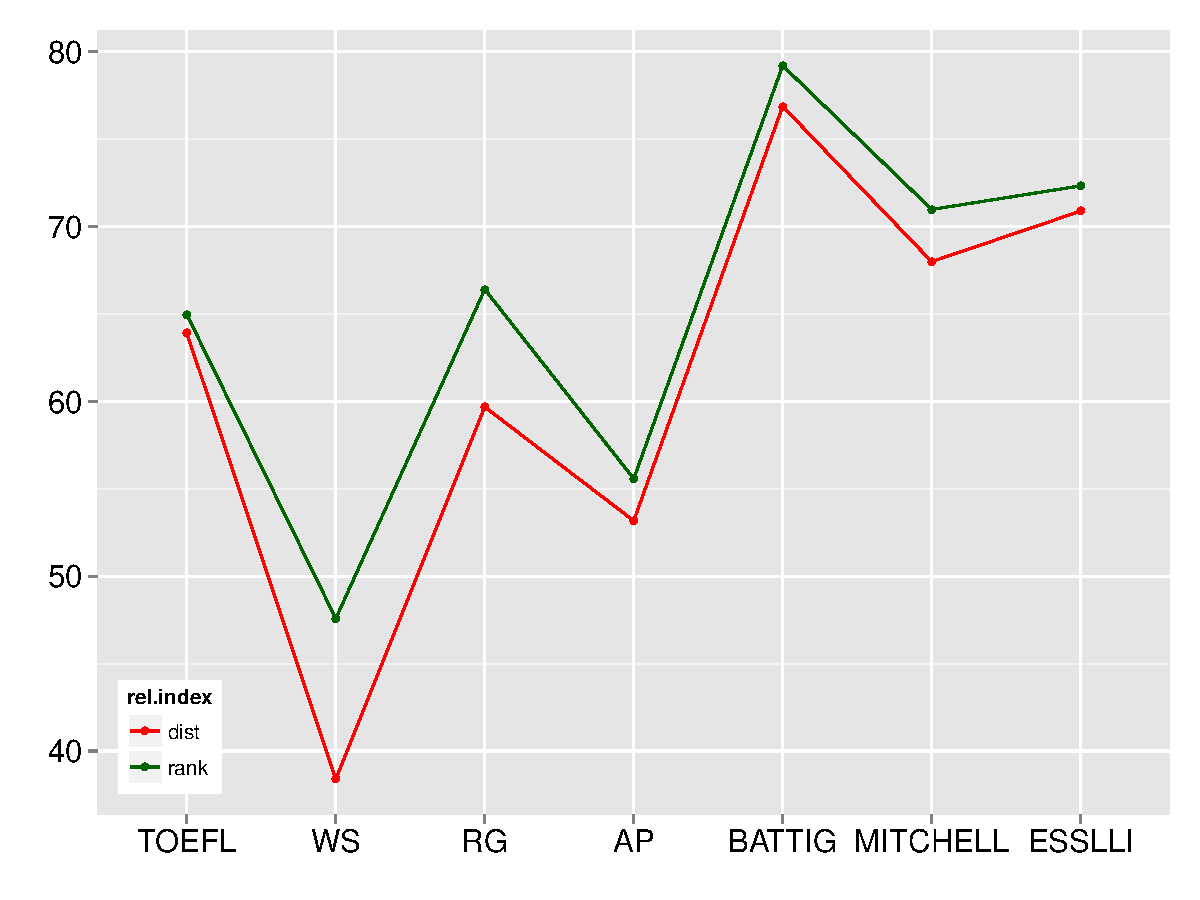
\includegraphics[scale=0.40]{img/lapesa_relindex_priming}
  \end{figure}   
  
\end{frame}

\begin{frame}
  \frametitle{Best settings and their performance}

  \begin{center}
    \setlength{\tabcolsep}{3.5pt}
    \footnotesize
    \begin{tabular}{lrlllllllllllllllll}
      \hline
      dataset & corpus & w &  o.dim & sc & tr & m  & rel.ind & n.dim & d.sk & best.s & best.m\\  \hline
      TOEFL & ukwac & \primary{2}  & 5k & s-ll & log & cos & rank  & \primary{900} & \primary{100} & 92.5 & 98.75 \\  
      WS & wacky & \primary{4} & 50k & s-ll  & log & cos & rank   & \primary{300} & \primary{50} &  0.67  & 0.73 \\ 
      RG &  wacky & \primary{4} & 50k & s-ll  & log & cos & rank   & \primary{300} & \primary{50} & 0.86  & 0.89 \\  
      AP & wacky & \primary{4} & 20k & s-ll & log & cos & rank   & \primary{300} & \primary{0} & 0.69 & 0.76 \\ 
      BATTIG & wacky & \primary{8}  & 50k & s-ll & log & cos & rank   & \primary{500} & \primary{0} & 0.98  & 0.99 \\ 
      ESSLLI & wacky & \primary{2} & 20k & t-sc & log & cos & rank   & \primary{300} & \primary{0} & \textit{0.77} & \textit{0.98} \\   
      MITCHELL & wacky & \primary{4}  & 50k & s-ll & log & cos & rank  & \primary{500} & \primary{0} & 0.88 & 0.97 \\   \hline 
    \end{tabular}

    \gap[1]
    \secondary{\normalsize Best settings for each dataset} 
  \end{center}
  
\end{frame}


\begin{frame}
  \frametitle{General settings}

  \ungap[1]
  \begin{center}
    \setlength{\tabcolsep}{3.5pt}
    \footnotesize
    \begin{tabular}{lrllllllllllllr}
      \hline
      task & corpus & w &  o.dim & sc & tr. & m  & rel.ind  & n.dim  & d.sk \\  
      \hline 
      TOEFL & ukwac & 2 &  5k & s-ll & log & cos & rank  & 900 & 100 \\   
      Rating & wacky & 4 & 50k & s-ll & log & cos & rank  & 300 & 50 \\  
      Clustering & wacky & 4 & 50k & s-ll & log  & cos & rank & 500 & 0 \\ 
      General & wacky & 4 & 50k & s-ll & log  & cos & rank & 500 & 50 \\ \hline 
    \end{tabular}

    \gap[1]
    \secondary{\normalsize General best settings} 

    \gap[2]
    \begin{tabular}{lccc>{\color{secondary}}c}
      \hline
      Task & TOEFL &  RATINGS &   CLUSTERING &  GENERAL  \\  
      \hline 
      TOEFL & 92.5 & 85.0  & 75.0 & 90.0   \\  
      WS & 0.60 & 0.67 & 0.64  & 0.68 \\  
      RG & 0.85 & 0.86  & 0.84 &  0.87 \\  
      AP & 0.60 & 0.66 & 0.67 & 0.67 \\  
      BATTIG & 0.85   & 0.91 & 0.98 & 0.90  \\  
      ESSLLI & 0.70 & 0.77  & 0.80 & 0.77  \\  
      MITCHELL & 0.73 & 0.83 &  0.88 & 0.83 \\ \hline     
    \end{tabular}

    \gap[1]
    \secondary{\normalsize General best settings -- Performance}
  \end{center}
  
\end{frame}

\begin{frame}
  \frametitle{Conclusion}
  \framesubtitle{Main findings}

  \begin{itemize}
  \item Our results show that it is possible to find a single DSM configuration that performs relatively well on every task
    \begin{itemize}
    \item[]
    \end{itemize}
  \item The most explanatory parameters show similar behavior across all tasks and datasets
    \begin{itemize}
    \item Simple-ll * Logarithmic Transformation 
    \item Cosine Distance
    \item[]
    \end{itemize}
  \item Parameters that show variation determine the amount and nature of the shared context
    \begin{itemize}
    \item Context window: 4 is a good compromise solution
    \item Dimensionality reduction: skipping the first dimensions\\ (but not too many) generally helps 
    \item Number of Feature Terms (to a lesser extent)
    \end{itemize}
  \end{itemize}
\end{frame}


\begin{frame}
  \frametitle{Conclusion}
  \framesubtitle{Main findings}
  
  \begin{itemize}
  \item Among the source corpora, WaCkypedia appears to be a better option than UkWaC for all tasks but TOEFL
    \begin{itemize}
    \item A good trade-off between quantity and quality?
    \item[]
    \end{itemize}
  \item As an indexe of distributional relatedness, neighbor rank is always better than distance, even if its contribution to model performance varies across tasks
    \begin{itemize}
    \item Perhaps some tasks/datasets are less asymmetric than others? 
    \item may need to exploit directionality in a more granular way
    \end{itemize}
  \end{itemize}
\end{frame}


%%%%%%%%%%%%%%%%%%%%%%%%%%%%%%%%%%%%%%%%%%%%%%%%%%%%%%%%%%%%%%%%%%%%%% 
%% References (if any)

\frame[allowframebreaks]{
\frametitle{References}
\bibliographystyle{natbib-stefan}
\begin{scriptsize}
  \bibliography{dsm,stefan-literature,stefan-publications}
\end{scriptsize}
}

\end{document}
